\documentclass[a4paper, twoside]{report}
\usepackage[utf8]{inputenc}

%% Language and font encodings
\usepackage[english]{babel}
\usepackage[T1]{fontenc}

%% Sets page size and margins
\usepackage[a4paper,top=3cm,bottom=2cm,left=3cm,right=3cm,marginparwidth=1.75cm]{geometry}

\usepackage[
backend=biber,
style=ieee,
sorting=none
]{biblatex}
\addbibresource{ref.bib}

% Command to get a normal looking # for F#
\newcommand{\fsharp}{{\fontfamily{phv}\selectfont \# }}

\newcommand{\codestyle}[1]{{\fontfamily{cmtt}\selectfont #1}}

%% Useful packages
\usepackage{amsmath}
\usepackage{algpseudocode}
\usepackage{algorithm}
\usepackage{float}
\usepackage{graphicx}
\usepackage{caption}
\usepackage{subcaption}
\usepackage[colorinlistoftodos]{todonotes}
\usepackage[colorlinks=true, allcolors=black]{hyperref}
\usepackage{titlesec}
\usepackage{listings}
\usepackage{wrapfig}
\usepackage{color}
%\usepackage{algorithmicx}
\usepackage{tabularx,array}
\usepackage[parfill]{parskip}
\usepackage{upquote}
\usepackage{multirow}
%\usepackage[altpo]{backnaur}
\usepackage[nounderscore]{syntax}
\usepackage{changepage}
\usepackage{tabularray}
\usepackage{pgfplots} 

\newenvironment{bnfsplit}[1][0.7\textwidth]
 {\minipage[t]{#1}$}
 {$\endminipage}
 
\lstdefinelanguage{FSharp}%
{morekeywords={let, new, match, with, rec, open, module, namespace, type, of, member, % 
and, for, while, true, false, in, do, begin, end, fun, function, return, yield, try, %
mutable, if, then, else, cloud, async, static, use, abstract, interface, inherit, finally },
  otherkeywords={ let!, return!, do!, yield!, use!, var, from, where, by },
  keywordstyle=\color{bluekeywords},
  sensitive=true,
  basicstyle=\ttfamily,
	breaklines=true,
  xleftmargin=\parindent,
  aboveskip=\bigskipamount,
	tabsize=4,
  morecomment=[l][\color{greencomments}]{///},
  morecomment=[l][\color{greencomments}]{//},
  morecomment=[s][\color{greencomments}]{{(*}{*)}},
  morestring=[b]",
  showstringspaces=false,
  literate={`}{\`}1,
  stringstyle=\color{redstrings},
}

\definecolor{bluekeywords}{rgb}{0.13,0.13,1}
\definecolor{greencomments}{rgb}{0,0.5,0}
\definecolor{redstrings}{rgb}{0.9,0,0}


%\setlength{\parindent}{0pt}

% \titleformat{\chapter}[display]
%   {\Huge\bfseries}
%   {}
%   {0pt}
%   {\thechapter.\ }
% \titleformat{name=\chapter,numberless}[display]
%   {\Huge\bfseries}
%   {}
%   {0pt}
%   {}

\title{FYP Interim Report}
\author{Aditya Deshpande }
\date{November 2021}

\begin{document}
\begin{titlepage}
                % \newgeometry{top=25mm,bottom=25mm,left=38mm,right=32mm}
                \setlength{\parindent}{0pt}
                \setlength{\parskip}{0pt}
                % \fontfamily{phv}\selectfont

                {
                                \Large
                                \raggedright
                                Imperial College London\\[17pt]
                                Department of Electrical and Electronic Engineering\\[17pt]
                                Final Year Project Report 2022\\[17pt]
 
                }

                \rule{\columnwidth}{3pt}
                \vfill
                \centering

                \setlength{\tabcolsep}{0pt}

                \begin{tabular}{p{40mm}p{\dimexpr\columnwidth-40mm}}
                                Project Title: & \textbf{Improving Issie} \\[12pt]
                                Student: & \textbf{Aditya Deshpande} \\[12pt]
                                CID: & \textbf{01504794} \\[12pt]
                                Course: & \textbf{EIE4} \\[12pt]
                                Project Supervisor: & \textbf{Dr Thomas J. W. Clarke} \\[12pt]
                                Second Marker: & \textbf{Mr S. Baig} \\
                \end{tabular}
\end{titlepage}
\clearpage
\pagenumbering{roman}
\section*{Acknowledgments}
TBA

\newpage

\chapter{Abstract}
TBA

\newpage

\tableofcontents
\clearpage
\pagenumbering{arabic}

\chapter{Introduction}

\section{Project Motivation}

Digital Electronics and circuit design are core fields in the study of Electronic Engineering, and are focused on the analysis and logical interpretation of digital signals, as well as the engineering of hardware that manipulates them in accordance with a desired logical function. A strong understanding of the fundamentals of digital electronics and circuit design serve as a foundation for multiple branches of study within Electronic Engineering. Therefore, it is vital that undergraduate students at Imperial College and other institutions have the best tools available to aid their study of these fundamental concepts.
One of the many challenges a first-year undergraduate student may face while learning Digital Electronic design is conceptualising relationships between inputs and outputs, and how these relationships relate to design specifications. At Imperial College London, EE students have the opportunity to gain a deeper insight into combinational logic through practical laboratory sessions, during which they create and simulate combinational circuits. The tools which they use must fulfil two criteria; firstly they must provide an education-focused platform through which students can learn more about combinational logic and hardware design; secondly they must be capable design tools in their own right which allow students to design and simulate complex logic.

Issie (Interactive Schematic Simulator with Integrated Editor) \cite{issie_repo}, an intuitive hardware design application, was developed at Imperial College London to address the lack of third-party programs that matched the above criteria. Issie is designed to be easy to use (requiring no user manual) and informative; visual cues and clear error messages guide students towards correct designs while individual step and waveform simulators allow students to vary inputs and see the effect on output values. This allows them to gain a better understanding of the hardware logic they have created. However, there is room for improvement.
In its current form, users of the application implement digital logic by building it component-by-component on a schematic diagram. Any syntactically correct digital circuit can be simulated using the \textit{Step Simulator}. In the Step Simulator, users specify values for each input to the digital logic, and can read the corresponding output values. Intermediate values can also be observed using \textit{Viewer} components. This functionality enables the user to easily verify their schematic with specific test cases, but lacks the ability to clearly summarise and verify the overall relationship between the inputs and outputs of the logic circuit. Users must therefore gain an overall understanding of the circuit through a combination of:
\begin{enumerate}
    \item Visually analysing the schematic to understand its logical function.
    \item Entering different input combinations into the Step Simulator and analysing the effect each change has on the outputs.
\end{enumerate}
As the implemented digital logic grows in complexity, the relationship between the inputs and outputs often becomes more obscure, and the schematic itself grows in size and can start to feel divorced from the specification. In such situations, the aforementioned method for understanding the logic circuit becomes less effective. To stop the schematic from getting too large and crowded Issie lets users define hierarchical \textit{Custom Components} which modularise the schematic and cut down on logic duplication. For example, an ALU may be implemented as a Custom Component within a CPU design schematic. This feature however, does not fully combat the issue of obscure relationships between inputs and outputs for complex circuits. Firstly, custom components that are not named clearly further obscure the logic function of the circuit. Secondly, due to their hierarchical nature, custom components can be nested inside other custom components, meaning that the user may have explore multiple layers of nested components before they can analyse the top-level schematic. This is a time-consuming exercise, requiring significant effort by the user. Therefore, there is significant value to adding functionality to Issie which allows users to better understand the relationships between inputs and outputs in digital logic circuits in a shorter amount of time.

One possible solution to this problem is automatically generating truth tables from the schematic. Truth tables exhaustively show the relationship between all inputs and outputs in an organised, persistent format. Inspecting cases in a truth table is far quicker than repeatedly changing values in the Step Simulator.
Furthermore, by investigating novel ways of presenting and interacting with these truth tables their value addition to the learning and circuit design experience in Issie can be boosted. For example, the ability to  present relationships inferred from the schematic in the truth table, or reduce an existing truth table with user-defined constraints, would provide the user with far more information than a simple simulation.

There is also merit in investigating the reverse; generating schematics from user-entered truth tables. This could reduce time spent designing hardware components which implement simple logic but require many gates and connections, as well as serve as a stepping stone between schematic design and HDL-based design.

Thus, there is a strong case for finding and implementing alternative ways to visualise (and possibly input) combinational logic in Issie to enable users to gain a better understanding of relationships in the logic, as well as the specification of the top-level design. If added in a way which compliments Issie's existing features, such enhancements are likely to increase Issie's effectiveness as an educational platform in addition to its capability as a a digital logic design tool.
This will benefit students at Imperial College and other educational institutions.

\section{Project Definition}

The purpose of this project is to explore novel ways in which interactivity can be added to automatic schematic-derived truth tables, and how interactively generated truth tables can be used as a fast aid to design combinational logic. This is to achieve the overall aim of this project - to improve Issie in such a way that it is easier for students to understand the use of logic in digital design.
The deliverable will be integrated as an extension to the Issie application, with users being able to generate truth tables from the schematic and interact with them in ways that will augment their understanding of the logic they are designing and of Digital Electronics concepts in general. 
This project will conduct a short evaluation of Issie, highlighting the areas where it can be improved. While the primary focus of the project is on visualising combinational logic with interactive truth tables, the project will also seek to improve the overall user experience of Issie in other ways such as tweaking/redesigning elements of the UI or changing how information is communicated to users such that it is consistent and clear. 
In addition to improving the user experience for Issie, this project also aims to improve the developer experience wherever possible. Since its inception, maintainability and extensibility have been key to Issie \cite{marco_diss}; therefore the code contributed to the Issie repository should be well-documented, readable, and interface well with existing code so that it is easy for future Issie developers to maintain and extend it. Further to this, if an appropriate opportunity arises, the project should also aim to reduce technical debt within the existing codebase.

\subsection{Core Principles of Issie} \label{subsec:principles}
As this project aims to improve Issie, any work done on this project should align with Issie's core principles. All features implemented in Issie must be:
\begin{enumerate}
    \item \textbf{Robust:} Software is robust when it is able to handle errors and behave correctly under exceptional circumstances, such as when supplied with erroneous inputs \cite{robust}. For simulations and text field inputs, Issie notifies the user of the nature of the error. User input, no matter how malformed, must never crash the application or lead to undefined behaviour.
    \item \textbf{Obvious:} The visual output given to the user should make it obvious what is happening without the need for unnecessary explanation. Issie prefers to \textit{show not tell} in order to remain beginner-friendly. For example, Issie uses colour-coded popups and highlights to draw user attention where it is needed and communicate events clearly.
    \item \textbf{Intuitive:} All functionality must be easy to expose to the user - there should be no need for detailed user guides as the UI for all functionality must be designed in a way such that users can intuitively learn how to use all of the application's features.
\end{enumerate}

In addition to these core principles, any extensions this project makes to Issie must also take into account the targeted users and the intended primary use case - teaching undergraduate students in a university laboratory while also enabling students to carry on where they left off at home. Thus, all new features must be cross-platform compatible and be suitable for students working in a laboratory and working alone at home.

In conclusion, this project has two final deliverables. The first is an improved version of Issie, while the second deliverable consists of appropriate documentation of added features, and improvements to the documentation of existing features.




\chapter{Background} \label{chap:background}
This chapter describes various theoretical concepts which provide context to many of the decisions made throughout the duration of the project. It also describes and evaluates the current version of Issie, analysing its strengths and weaknesses. Given the overall project goal of improving combinational logic visualisation in Issie, this analysis provides context for the extensions made to Issie by the project, which are described in subsequent chapters.
\section{Pedagogical Considerations} \label{sec:ped_cons}
Given the overall project aim of making it easier for students to understand the use of logic in digital design, any features added to Issie must enhance the learning experience of its users. Many decisions related to the project, such as which features to add, the UI/UX design, and the level of interactivity will all be made through the lens of pedagogy.
\subsection{Memory Models} \label{subsec:memmodels}
One of the key facets of learning is the long-term retention of key concepts and relationships. The Atkinson-Shiffrin multi-store model \cite{memory_model} provides a good framework for modelling the workings of human memory, and many task-specific models, theories, and techniques have been derived from it. The aim of any effective learning application should be to convey and revisit information in such a way that it succeeds in reaching the Long Term Memory store.

\begin{figure} [h]
    \centering
    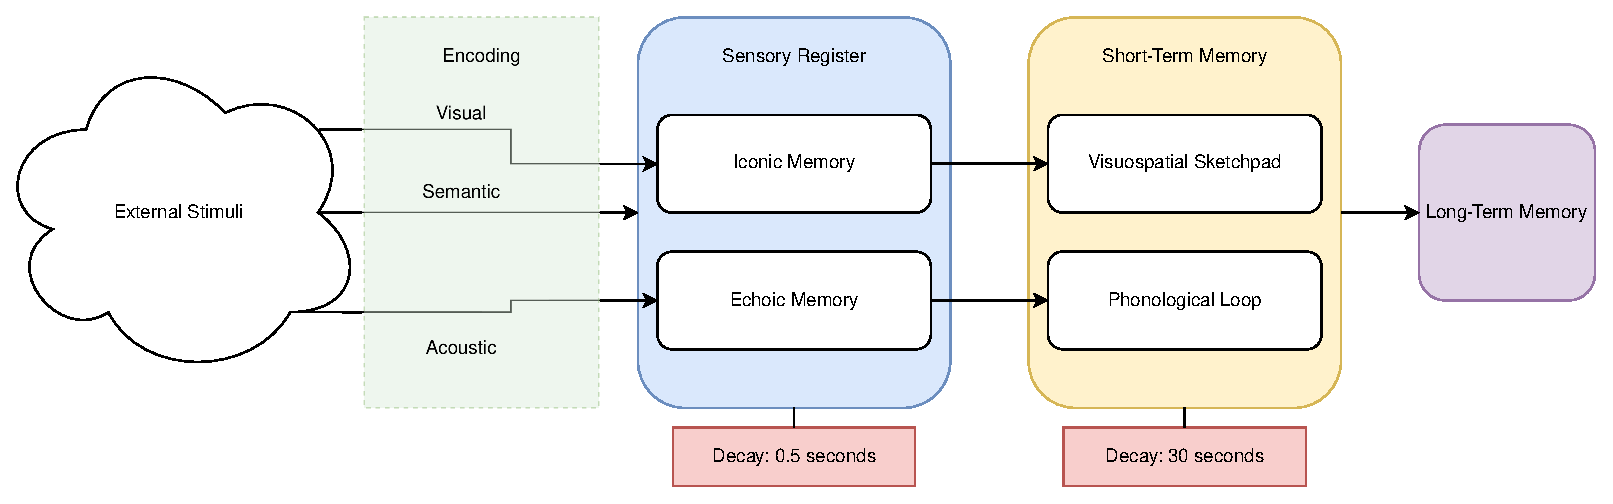
\includegraphics[width=\textwidth]{02.Background/atkinson.eps}
    \caption{The Atkinson-Shiffrin Multi-Store Model}
    \label{fig:atkinson}
\end{figure}

As shown in Figure \ref{fig:atkinson}, the Atkinson-Shiffrin Multi-Store Model states that humans perceive information through external stimuli, and that information is encoded as three different types of stimulus. \textbf{Visual} encoding encodes information in pictures and diagrams, \textbf{Semantic} encoding encodes information in words and their meanings, while \textbf{Acoustic} encoding encodes information in sounds. This encoded information is processed by the sensory register. If attention is paid to this information, it travels into short-term memory, otherwise it decays within half a second and is forgotten. For information to progress from short-term to long-term memory, a process of repetition called maintenance rehearsal is necessary \cite{multi_store}, in which the information is repeated within the learner's mind. For visually encoded information, this could be through repeated visualisation of diagrams or patterns in what the learner sees on a screen, while for acoustically encoded information this is achieved through the learner playing back the soundbite in their head (phonological loop). A key take-away from this memory model is that human brains process different information encodings independently, meaning that even if one encoding type is saturated with information, additional information can still be conveyed to the learner using an alternative encoding method. 

In its current form, Issie encodes information about the digital circuit both visually (circuit diagram, error highlighting etc.) and semantically (error messages, simulation outputs). No information is encoded acoustically, however outside of chimes for errors there is not much scope for implementation of sounds. Furthermore, students will receive plenty of auditory information in the form of teaching from lab assistants and conversation with their peers. Any extensions added to Issie by this project should therefore focus on conveying information to users through a combination of diagrams with appropriate annotations and informative text.

\subsection{Educating Engineers} \label{subsec:educating_engineers}
As a tool for teaching Digital Electronics, Issie's primary user base is engineering students. Therefore, there is value in exploring trends in how engineers learn best, and tailoring Issie's design and structure to align with these trends.
In 1992, Fleming and Mills proposed that there were four categories of how students learned. These are \textbf{visual}, \textbf{auditory}, \textbf{reading/writing}, and \textbf{kinesthetic} \cite{Fleming1992}. Most learners will learn using all of these methods, however will exhibit a preference towards one or two. Studies have shown that engineers have a preference towards visual and kinesthetic learning techniques \cite{vark_engineers}. The visual aspect means that engineers prefer information be conveyed to them through diagrams, patterns, and highlighted meaningful symbols. On the other hand, the kinesthetic aspect means that engineers prefer to learn through demonstrations, simulations, and their own experiences. The existence of practical lab sessions and Issie itself lends itself to a focus on kinesthetic learning; students explore concepts they have been taught about in lectures by building and simulating combinational logic. Therefore, the results of the VARK survey concur with the current teaching style in the EEE Departement at Imperial College. Currently, Issie has an interactive diagram with highlighting (visual encoding), as well as simulators for testing logic and general experimentation (kinesthetic learning). Thus, it can be said that Issie in its current form is fit for its purpose: educating engineers. In turn, any extensions added to Issie by this project should continue this trend of visual and kinesthetic learning, but while also taking care to not overload the users' sensory register and short-term memory.

\subsection{Cognitive Theories of Self Efficacy and Constructivism} \label{subsec:self_efficacy}
There are more factors that contribute towards an effective learning experience than just the conveyance of information. The learning process must be structured in such a way that students remain motivated while learning complex concepts. A ten-year longitudinal study \cite{motivation} found that there is a significant correlation between students who are motivated, therefore having high self-confidence, and academic attainment. Therefore, while developing educational tools like Issie, an emphasis must be placed on communicating information to students in such a way that they retain the belief that they can successfully learn the content. This approach aligns well with the theory of constructivism in education, which seeks to educate students by having them discover knowledge intuitively in contrast to traditional methods in which a student is considered an 'empty vessel' waiting to be filled up by a teacher \cite{construct}. The rationale behind the theory is that this self-discovery of knowledge will build a stronger conceptual understanding of what is being learnt. Constructivism aligns well with teaching styles that suit kinesthetic learners, as both approaches focus on students learning through their own experiences. Engineers tend to be kinesthetic learners, therefore, this project should aim to improve Issie in such a way that students are able to interactively and iteratively build their understanding of digital electronics and circuit design by themselves.

\section{Combinational Logic}
Combinational logic is a type of digital logic in which the output of the logic is a pure function of its present inputs \cite{comblog_wiki}. This means that combinational logic is memoryless; it is not affected by any previous outputs. This is in contrast to sequential logic, for which the output is dependent on present input values and some internal state derived from previous outputs.

\subsection{Visualising Logic with Boolean Algebra}
The aforementioned pure function which maps inputs to outputs can be written as a Boolean expression. A Boolean expression, much like traditional mathematical expression, features a set of input terms combined using operators. There exist three fundamental Boolean operators \cite{gregg_boolean}:
\begin{itemize}
    \item[] \textbf{NOT}, a unary operator which outputs the inverse of the input.
    \item[]\textbf{AND}, a binary operator which outputs HIGH when both inputs are HIGH and LOW otherwise. Denoted by 
    \item[] \textbf{OR}, a binary operator which outputs HIGH when either of the inputs are HIGH, and LOW otherwise
\end{itemize}
Other Boolean operators, such as \textbf{NAND}, \textbf{NOR}, and \textbf{XOR} also exist, but can be defined using a combination of the three fundamental operators.
Therefore, the first and most basic way of visualising combinational logic is simply through writing the Boolean expression which represents it. However, it can be difficult to quickly understand what some logic does using just Boolean expressions. Take for example the following Boolean equation for output $Y$, derived from inputs $S$, $A$, and $B$:
\begin{equation}
       Y = \overline{S}.A + S.B
       \label{equ:MuxEq}
\end{equation}
While the operations performed are clear, it may not be very clear on first inspection to an inexperienced student what the expression actually achieves. Furthermore, Boolean expressions grow in complexity as schematics become larger, making them even tougher to understand at a glance.

\subsection{Visualising Logic with Schematic Diagrams}
Schematic diagrams give the hardware representation of the combinational logic, and are the primary way of creating and visualising combinational logic in Issie. At their simplest, they consist purely of logic gates; these gates each correspond to a Boolean operator. However, in practice (and Issie) schematics are at a slightly higher-level, with certain combinational components (which can be built from gates) pre-created for the user. For example, Equation \ref{equ:MuxEq} represents a 2-bit Multiplexer, which is a component available in Issie's catalogue. The recall of stored knowledge due to the visual stimulus of the multiplexer component on the diagram is much more likely compared to the semantic stimulus of the Boolean expression. However, as a schematic increases in size, the number of components may become so large that holding all of the visual stimuli in short-term memory is unfeasible. Issie combats this by letting users modularise their schematic through hierarchical custom components. Alongside decreasing schematic size and repeated logic, this feature actually aims to teach students the technique of modularising their work (whether that is a schematic or code), and its advantages. These advantages \cite{arm_modular} include efficient development, easier dubugging, and logic reuse. However, as mentioned in the Project Motivation, hierarchical components are not always effective (particularly if badly named and organised), leaving a opportunity for improvement through complementary visualisation techniques. 

\section{Truth Tables} \label{subsec:TruthTables}
A truth table represents a given combinational logic function; featuring all input combinations on the left, and their corresponding output(s) on the right. As the truth table maps all possible inputs to their output, it is trivial to look up the behaviour of the logic in a given scenario. A very basic example is the truth table for the Boolean \textbf{AND} operator, shown in Table \ref{tab:And_TT}.

\begin{table}[h!]
    \centering
    \begin{tabular}{c|c||c}
     \textbf{A} & \textbf{B} & \textbf{C} \\
     \hline
     0 & 0 & 0  \\
     0 & 1 & 0  \\
     1 & 0 & 0  \\
     1 & 1 & 1
    \end{tabular}
    \caption{Truth Table for the Boolean AND operator ($C = A.B$)}
    \label{tab:And_TT}
\end{table}

Given that a truth table defines some logic using an exhaustive set of examples, it could be said that truth tables are ideal for kinesthetic learners. This exhaustive property can also be used to test for logical equivalence. Suppose the claim is made that two schematics, with one schematic featuring far fewer components than the other, are logically identical. Equivalence could be confirmed by simply checking if the truth tables for the two schematics are the same. 

However, a disadvantage of using truth tables to visualise combinational logic is that they can very rapidly grow in size. For logic with $n$ single-bit inputs, the number of rows in the associated truth table is $2^n -1$. For multi-bit inputs this number would grow even larger. Thus, Issie schematics with a large number of inputs would result in very long truth tables, which would likely intimidate the user. The size of generated truth tables could be reduced by filtering them based on user selections, or through truth table reduction methods.   

\subsection{Reduction using Don't Cares} \label{subsec:dcbackground}
A "Don't Care" term in a truth table can mean different things based on it's positioning. It is more commonly seen on the right-hand side of a truth table, signifying that an output for a given input combination is invalid or has no use \cite{1969logic}. This information is often used when attempting to simplify Boolean expressions using Karnaugh maps. On the other hand, a Don't Care term in an input row signifies that the particular input has no effect on the eventual output of the logic for that combination. These \textit{Don't Care inputs} can be found through logic minimisation, of which there are numerous techniques ranging from the aforementioned Karnaugh Maps \cite{kmapbook} to heuristic-based tools like Espresso \cite{espresso}. The latter is very effective at reducing large circuits efficiently, and would therefore appear to fit the needs of the project well. An example of the reduction can be seen in Table \ref{tab:muxTTs}, where the eight row exhaustive truth table (\ref{subfig:muxTT_standard}) is reduced to two rows (\ref{subfig:muxTT_dc}). However, Espresso and other common minimisation techniques treat their inputs and outputs as single-bit Boolean values which are either \codestyle{ON}, \codestyle{OFF}, or \codestyle{DC} -- corresponding to 1, 0 and Don't Care \cite{espressoinputs}. Multi-bit IOs are broken into their constituent bits. In Table \ref{subfig:muxTT_dc}, only HIGH outputs are shown -- this works when it can be assumed that all other input combinations yield 0. This approach aligns well with industrial applications, where signals on wires can only be HIGH or LOW, and there is value in reducing to the form which requires the fewest gates.  On the other hand, Issie is an educational application where inputs and outputs can have more than two values, and focus is more on semantics and understanding rather than the most cost-efficient hardware design. Therefore, such minimisation would not integrate well with Issie's existing implementation of multi-bit IOs.

In order to implement DC reduction in Issie, a suitable algorithm will have to be written which supports multi-bit inputs. One possibility may be analysis of redundancies in the existing truth table. For example, in the full truth table, the first and third row both have an output value of 0, with the only difference being the change in the value of $B$. Given that $B$ can only take two values, this shows that when $A=0$ and $S=0$, the value of $B$ does not affect the output - therefore we "don't care" about B. Rows one and three can therefore be collapsed into one row, with the entry for the $B$ column being replaced with an "X". This process can be repeated until all such row combinations have been collapsed. The results from this process can be seen in Table \ref{subfig:muxTT_dc_zeros}. The length of the truth table has been reduced by 25\%, and the actual semantic function of what the multiplexer does is much clearer as well. This table is however, much larger than the reduced table generated by Espresso, indicating that it may not work well with larger schematics.

\subsection{Algebraic Truth Tables}
While reduction with Don't Cares is useful, neither implementation of it is ideal. Industry-style minimisation doesn't fully align with Issie's implementation, while custom algorithms may not be reduce the table enough. Additionally, Don't Care reduction cannot simplify relationships which involve all inputs, such as arithmetic. A viable alternative is an Algebraic Truth Table; these are often found on component datasheets \cite{timux} and have the task of summarising the behaviour of the circuit in a concise and readable format.  One such example is shown in Figure \ref{fig:datasheet}, which is an excerpt from a datasheet for a three-input multiplexer. H and L are equivalent to 1 and 0, but the terms of form $I_x$ in the table are algebraic values representing inputs. The select signals ($S2,S1,S0$), which actually control the circuit behaviour are still numeric.

\begin{figure}[h]
    \centering
    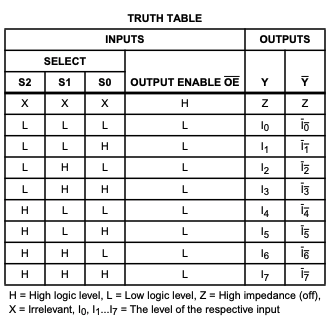
\includegraphics[width=0.5\textwidth]{02.Background/datasheet.png}
    \caption{Algebraic Truth Table in Datasheet for a Three-input Multiplexer \cite{timux}}
    \label{fig:datasheet}
\end{figure}

Table \ref{subfig:muxTT_alg} shows what the corresponding algebraic truth table would look like for the running example in this section.
$A$ is propagated to the output when the selection input ($S$) is low, and $B$ is propagated when $S$ is high. This clearly describes a two-input multiplexer. Having functionality which could create similar tables for user-created schematics, with support for more complex algebraic operators would likely be useful. This is because algebraic truth tables carry far more semantic information in a much smaller visual space, meaning that a students' sensory register is less likely to be overloaded.

\begin{table}[h]
    \centering
    \subfloat[Full Truth Table]{
    \label{subfig:muxTT_standard}
    \begin{tabular}{c|c|c||c}
     \textbf{A} & \textbf{B} & \textbf{S} & \textbf{OUT} \\
     \hline
     0 & 0 & 0 & 0 \\
     0 & 0 & 1 & 0 \\
     0 & 1 & 0 & 0\\
     0 & 1 & 1 & 1\\
     1 & 0 & 0 & 1\\
     1 & 0 & 1 & 0\\
     1 & 1 & 0 & 1\\
     1 & 1 & 1 & 1\\
    \end{tabular}}
    \medskip
    \subfloat[DC Reduced \\(Inc. Zeros)]{
    \label{subfig:muxTT_dc_zeros}
    \begin{tabular}{c|c|c||c}
     \textbf{A} & \textbf{B} & \textbf{S} & \textbf{OUT} \\
     \hline
     0 & X & 0 & 0 \\
     X & 0 & 1 & 0 \\
     X & 1 & 1 & 1\\
     1 & X & 0 & 1\\
     0 & 0 & X & 0 \\
     1 & 1 & X & 1
    \end{tabular}}
    \medskip
    \subfloat[DC Reduced \\(Espresso)]{
    \label{subfig:muxTT_dc}
    \begin{tabular}{c|c|c||c}
     \textbf{A} & \textbf{B} & \textbf{S} & \textbf{OUT} \\
     \hline
     1 & X & 0 & 1 \\
     X & 1 & 1 & 1
    \end{tabular}}
    \medskip
    \subfloat[Algebraic Truth Table]{
    \label{subfig:muxTT_alg}
    \begin{tabular}{c|c|c||c}
     \textbf{A} & \textbf{B} & \textbf{S} & \textbf{OUT} \\
     \hline
     A & B & 0 & A \\
     A & B & 1 & B
    \end{tabular}}
    \caption{Truth Tables for a 2-bit Multiplexer}
    \label{tab:muxTTs}
\end{table}


\section{An Overview of Issie's Technology Stack} \label{sec:techstack}

The reasoning and process behind the decisions made for Issie's technology stack can be found in Marco Selvatici's dissertation on DEFlow, the predecessor to Issie \cite{marco_diss}. This section describes the technology stack, and evaluates and reaffirms why Issie's technology stack is well suited.

\subsection{Programming Language} \label{subsec:fsharp}
Issie is written in F\fsharp, an open-source, cross-platform, interoperable programming language for writing succinct, robust and performant code \cite{fsharp}. It is functional-first; meaning that it contains many features found in functional languages and encourages a functional programming style while also allowing programmers the flexibility to use the programming styles of other paradigms. Pure functional programming languages adopt a philosophy of declarative programming and immutable data; data values cannot be updated after initial assignment, and functions take this data as input and map it to output data. These functions are deterministic, meaning that their output is solely dependent on the value of their inputs and that there is no internal state affecting the behaviour of the function. This differs from the more common imperative style of programming where code is treated as a sequential list of instructions which mutate program data/state. The deterministic nature of functions in pure functional programming makes them very easy to understand, as operations on data have no side-effects and are therefore very easy to track. Not only does this make debugging easier, but it leads to fewer overall bugs in the code. A large-scale study of programming languages and code quality on Github \cite{functionaldebug} found that "Functional languages have a smaller relationship to defects than other language classes, whereas procedural languages are either greater than average or similar to the average." The study also found that the "Functional-Static-Strong-Managed" class of languages (i.e. languages that are functional, statically and strongly typed with in-built memory management) are  less likely than average to result in defect-fixing commits on Github.
While not a part of the study, F\fsharp does belong to this class of languages, and is therefore a wise choice of programming language for Issie. F\fsharp features a Hindley-Milner type system, which has a provably sound type inference algorithm \cite{hm_typesis}. Type inference allows for F\fsharp to be statically typed while eliminating the need for type annotations in the code. This results in clean-looking and succinct code while still maintaining the benefits of static typing.  Furthermore, as types can be inferred on the fly by IDEs such as Visual Studio, it is much easier for the programmer to track the correctness of the program. 

\begin{wrapfigure}{l}{0.5\textwidth} 
  \begin{center}
    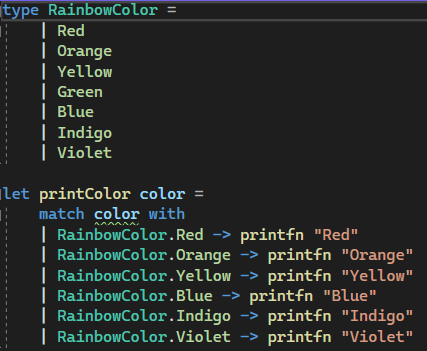
\includegraphics[width=0.40\textwidth]{02.Background/patternmatch.png}
  \end{center}
  \caption{An example of incomplete Pattern Matching in F\fsharp, with a warning from the compiler}
  \label{fig:patternmatch}
\end{wrapfigure}

One such example is found when pattern matching, as seen in Figure \ref{fig:patternmatch}. The function \codestyle{printColor} takes as input some colour of the rainbow (type \codestyle{RainbowColor}) and prints the colour. \codestyle{RainbowColor} is an F\fsharp Discriminated Union (DU) type \cite{dutypes}, where the data stored in the value is not fixed; it can be one of several distinct options. DU types have many applications, ranging from representing valid and error cases to small object hierarchies.  The type system allows for the IDE to first infer the type of the variable \codestyle{color}, and then realise that the pattern match does not cover the DU case for when \codestyle{color} is Green. Mousing over the warning line in Visual Studio gives the following message: "Incomplete pattern matches on this expression. For example, the value 'Green' may indicate a case not covered by the pattern(s)." Such hints are immensely useful for the programmer. The advantage of such checks being performed before and at compile-time is that it decreases the number of errors at run-time, which tend to be more disruptive.

F\fsharp also helps protect against runtime errors through the use of Monadic types. Sometimes, certain actions in a program may need to return \textit{nothing}, such as an unsuccessful lookup in a Map/Dictionary or if there is an absence of some data. Usually such messages are communicated within the program using either exceptions or NULLs which have to be caught and handled. If not tracked and handled appropriately, NULLs in particular can lead to some very nasty and hard-to-debug runtime errors. F\fsharp allows programmers to minimise the use of exceptions and avoid the use of NULLs using the \codestyle{Option} and \codestyle{Result} types. The \codestyle{Option} type can take the value \codestyle{Some <type a>} or \codestyle{None}, giving the programmer a safe way to indicate nothing without using NULLs. The \codestyle{Result} type can reflect success (\codestyle{Ok <type a>}) or failure (\codestyle{Error <type b>}), giving the programmer a safe way to propogate errors through their code without raising exceptions or returning NULL. 

While F\fsharp has the many features and benefits of pure-functional languages and strongly encourages the programmer to use them, it is an impure functional language and does allow the programmer to use other styles of programming. For example, mutable state in functions is allowed by the use of the \codestyle{mutable} keyword upon definition. This allows flexibility; programmers can use the default functional style in most places, and can selectively choose where to introduce functionally impure constructs such as mutable state. An example of this in Issie is the \textit{FastSimulation} used by the Step Simulator, which uses mutable arrays to represent the value of component inputs/outputs at different clock cycles.

As most of the features mentioned in this section are either unique to or far better implemented in F\fsharp compared to other common app development languages such as JavaScript or Python, and that F\fsharp belongs to the most bug-free class of languages, it can be said that Issie's choice of programming language is apt and ideal.

\subsection{Ecosystem} \label{subsec:ecosystem}
While originally built as a language for the .NET framework, built to run on the Microsoft Common Lanugage Runtime (CLR) \cite{clr_mag}, F\fsharp can also execute in Javascript environments through the use of third-party trans-compilation tools \cite{fableio}. Therefore, F\fsharp can be used to build desktop applications using .NET, as well as Javascript web apps. Issie is built using the latter method; F\fsharp code is compiled to JavaScript, which is executed in a desktop environment through Electron. This section describes the chosen tools in this process, and the reasoning behind those choices.

\subsubsection{Electron}
Electron \cite{electrondocs} is a framework for building desktop applications using JavaScript, HTML, and CSS. Electron comes bundled with the open-source Chromium browser and Node.js, a runtime environment that lets JavaScript code execute outside of a browser. Using these, Electron enables web apps to run locally on the user's machine outside of a web browser, akin to a native program. The advantage of this approach is that a developer can create a cross-platform application without any experience of programming native applications for any platform. On the other hand, pure native desktop applications often require differing codebases if multiple platforms are to be targeted \cite{webapps}; this is a far more labour-intensive approach which also requires a wider skill set. Common native desktop application technologies, such as UWP and WPF, have a much steeper learning curve compared to Electron as well \cite{mustdecisions}. Given that Issie is maintained by various students over time, an ecosystem that allows for easy cross-platform development with a relatively shallow learning curve is preferable, making Electron well suited for Issie's ecosystem.

However, potential issues with Electron must also be discussed. As Electron apps bundle Chromium and Node, they are often quite large. Additionally, due to the use of the RAM-intensive Chromium browser, Electron apps tend to use more memory than other similar applications \cite{roryok}. This could lead to decreased performance on low-end hardware. Electron is also dependent on a large amount of open-source code, and web apps are often very reliant on Node dependencies, which can change at any time. This reliance could also be perceived as a weakness.

However, despite some of its shortcomings, Electron is still a good fit for Issie's use case. Issie in its current form is performant, responsive, and stable; implying that the performance issues with Electron have not affected Issie significantly enough for there to be notable issues. The advantage of easy cross-platform development, as well as good integration with Fable (which allows F\fsharp to be used as the programming language), outweighs the risks posed by potential Node dependency issues, as well as a larger app footprint.

\subsubsection{Fable}
While Electron provides a convenient framework for building cross-platform applications, it requires a JavaScript codebase. JavaScript is a weakly and dynamically typed imperative language - making it a sub-optimal choice for the development of Issie. The gap between development and deployment is bridged by \textbf{Fable} \cite{fableio}, a compiler that brings F\fsharp to the JavaScript ecosystem. Fable compiles F\fsharp to clean JavaScript code which can run under Electron. Fable also includes bindings for React \cite{reactjs}, a highly performant JavaScript library for building user interfaces; this allows Issie's F\fsharp code to create React elements which Fable will compile to their respective JavaScript implementations.

\subsection{User Interface and Rendering}
A well-written and structured Graphical User Interface (GUI) is an essential component of any application, but it becomes even more vital in the context of an application like Issie which prioritises an interactive and intuitive interface. In Issie, most of the user's interaction with the program is done using the mouse; clicking, dragging, and hovering. This means that the UI code must be able to handle a constant stream of pseudo-random mouse events and deal with them quickly and appropriately. It must also be maintainable and extensible to easily allow for more functionality to be added over time. This section describes the workings of Issie's UI framework, as well as the reasoning behind the decision to choose the framework.

\subsubsection{Elm, Elmish, and MVU}
The Elm Architecture \cite{elmarch}, also known as the MVU Architecture, is a pattern for creating interactive programs which emerged from the Elm programming language. Elm \cite{elm} is a purely functional language for creating websites and web apps. Elm compiles to JavaScript - this is similar to how using F\fsharp with Fable allows functional F\fsharp code to be compiled to JavaScript for a web app. Issie uses the Elmish library \cite{elmishdocs}, which brings Elm's MVU architecture to F\fsharp and integrates well with Fable, enabling Issie's smooth and robust GUI.

The MVU architecture gains its name from the three parts it splits the UI code into:
\begin{itemize}
    \item[] \textbf{Model:} A data structure which stores the state of the application. In Issie this is a very large record, containing lots of information ranging from the results of a simulation to which components are selected and highlighted.
    \item[] \textbf{View:} A pure function which specifies how the information in the model (application state) should be displayed to the user. The developer writes a function to turn the model into HTML/CSS equivalents, and Elm (or Fable if using F\fsharp with Elmish) converts this to actual HTML/CSS and renders it. 
    \item[] \textbf{Update:} A way to update the application state triggered by events such as user input. These events are communicated within the program using \textit{messages}, which are triggered by the user interacting with the GUI. The update function is a  pure function which accepts two parameters, the incoming message and the current model. It then interprets the message and returns an updated version of the model. 
\end{itemize}

An initial Model is specified in the code, which is rendered by the View function on application startup. The user can then interact with the application - each interaction will generate a message which is passed to the update function. The update function processes this message and, if required, will return an updated model which reflects the effects of the interaction. On its next invocation, the View function will render this updated application state, showing the user the result of their interaction.

The MVU Architecture has numerous strengths, many of which make it suitable for use in Issie. It's structure, based on an immutable Model with deterministic (pure) View and Update functions, means that data flows in only one direction through the whole application, while events which warrant a change in the application state are clearly marked as messages. This making the rendering process easier to understand for the programmer \cite{mvuthesis}, meaning that more time is spent writing useful code instead of debugging. This is unsurprising given that Elm, like F\fsharp, is a functional language, and therefore belongs to the "Functional-Static-Strong-Managed" class of languages mentioned in Section \ref{subsec:fsharp}. F\fsharp also has features which integrate well into the MVU architecture, strengthening it further. One such example is F\fsharp's strict compile order, which helps avoid cyclic references between view subfunctions \cite{mvuthesis}. Altogether, the MVU architecture is a good fit for Issie, improving the developer experience while delivering a performant UI.

On initial inspection, the design decision of having a View function which repeatedly re-renders the Model every time there is some update appears inefficient. This would be the case if Elm (and other implementations of MVU) used the traditional process for rendering a web page/app.
This traditional process for rendering HTML is shown in Figure \ref{fig:tradDOM}. The HTML is parsed and a DOM (Document Object Model) is constructed; this is a tree representation of the HTML. Whenever the website/web app state changes, certain parts of the generated HTML change too. The DOM tree must be updated to reflect these changes, however this is often a slow process for large web apps with a large number of nodes in the DOM tree, resulting in the UI appearing sluggish. Elm combats this by using an intermediate \textbf{Virtual DOM}, a lightweight and optimised version of the main DOM tree on which operations are cheap. As shown in Figure \ref{fig:virtualDOM}, Elm exposes this virtual DOM to the programmer, who specifies how the state should be viewed in the View function. For each change of state, a new virtual DOM is constructed and compared to the previous virtual DOM. Through this, Elm can determine the exact change to the UI. Both the construction and comparison are fast due to the lightweight nature of the virtual DOM. Elm repeats this process for multiple changes to the UI, creating a batch of updates to be performed on the actual DOM tree at once. This method significantly reduces the per-update penalty for updating the DOM, allowing for efficeint re-rendering of the program state. This improves the performance of the web app. Another advantage of this method is that the task of efficiently updating the DOM is abstracted away from the programmer, leaving them with only the task of specifying how their website or web app should look.

\begin{figure} [h]
    \centering
    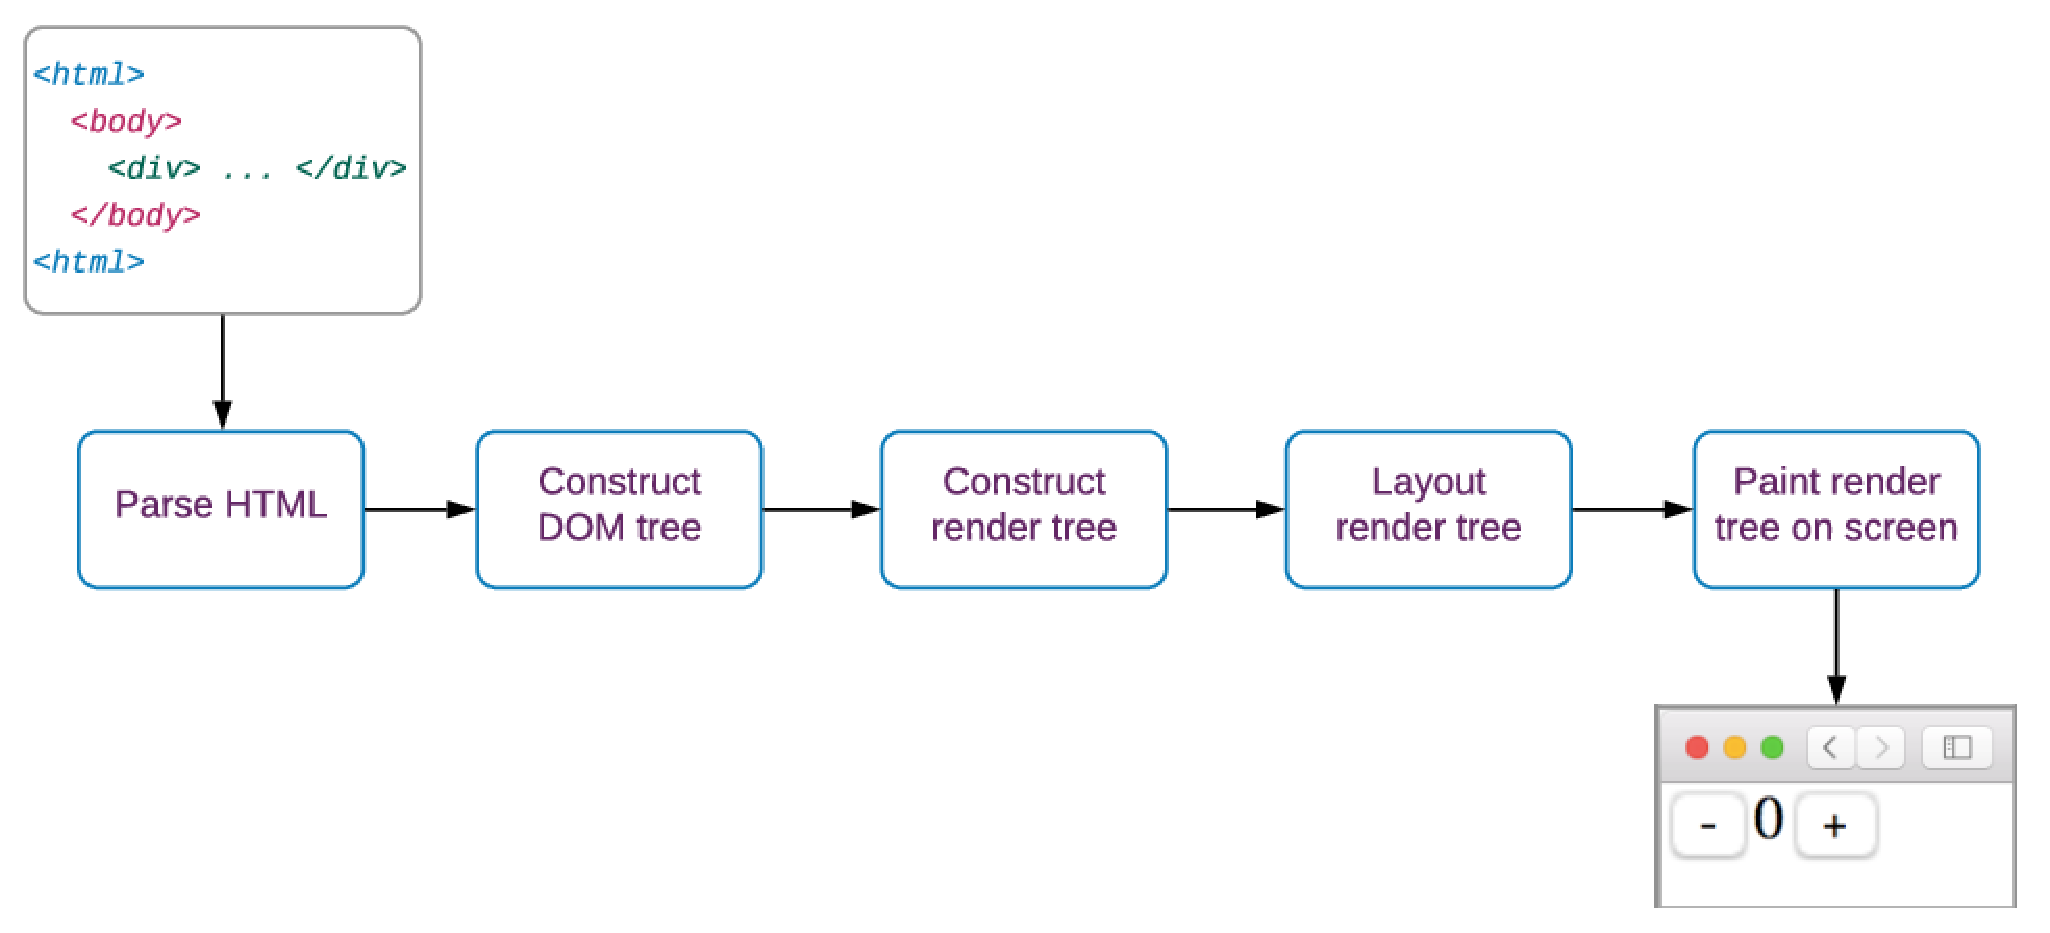
\includegraphics[width=\textwidth]{02.Background/traditionalDOM.eps}
    \caption{How browsers traditionally render HTML using a DOM \cite{virtualdom}}
    \label{fig:tradDOM}
\end{figure}

\begin{figure} [h]
    \centering
    \includegraphics[width=\textwidth]{02.Background/elm-virtual-dom.eps}
    \caption{The Elm Architecture \cite{virtualdom}}
    \label{fig:virtualDOM}
\end{figure}

\subsubsection{React}
React, as mentioned earlier, is a library for building user interfaces. In the Issie project, Elmish uses React for rendering the UI due to its efficient virtual DOM. Thus, the virtual DOM mentioned previously is actually the React Virtual DOM, which is a tree of React Elements. React Elements are simple objects, and are therefore cheap to create \cite{reactrender}, meaning that operations on the React DOM are computationally inexpensive. The View function returns a React Element which shows the current state of the UI. React improves the performance of an application by only re-rendering elements when necessary. The React equivalent of the process mentioned previously where virtual DOMs are compared to find UI changes is called \textit{Reconciliation} \cite{reactrender}.

React also provides a further method for increasing performance: memoization \cite{reactcache}. Memoization is most useful when working with components whose state is partially dependent on computationally intensive calculation. Under traditional React, this value would be re-calculated on every render, even if it had not changed. This increases the amount of time each render takes. An example of this would be the result of the addition of two very large numbers ($a + b$), which is a very CPU intensive task. Memoization combats this by caching the previous value of the computation and only performing the calculation whenever $a$ or $b$ changes. Issie already uses some memoization in its code for the Step Simulator: after a sheet is simulated for the first time the simulation is cached. If the sheet hasn't changed the next time a simulation is started, the cached simulation is used instead of building a new one, increasing performance. 
\subsubsection{Fulma} \label{subsec:fulma}
Fulma \cite{fulmaio} is an F\fsharp library which provides a wrapper around Bulma \cite{bulmaio}, an open-source CSS framework which provides ready-to-use front-end components for building responsive web interfaces. Fulma brings these components to F\fsharp for use with Fable React. React components such as buttons, forms, and tables can easily be specified in the F\fsharp code using the functions provided by Fulma. Listing \ref{lst:fulmatable} shows the F\fsharp code for generating a table using Fulma, while Figure \ref{fig:fulmatable} shows the rendered table.

\begin{lstlisting}[language=FSharp, caption={Simple F\fsharp code for generating a table with Fulma \cite{fulmatable}}, captionpos=b, label={lst:fulmatable}]
    Table.table [ Table.IsBordered
              Table.IsNarrow
              Table.IsStriped ]
    [ thead [ ]
        [ tr [ ]
             [ th [ ] [ str "Firstname" ]
               th [ ] [ str "Surname" ]
               th [ ] [ str "Birthday" ] ] ]
      tbody [ ]
        [ tr [ ]
            [ td [ ] [ str "Maxime" ]
              td [ ] [ str "Mangel" ]
              td [ ] [ str "28/02/1992" ] ]
          tr [ ClassName "is-selected" ]
             [ td [ ] [ str "Jane" ]
               td [ ] [ str "Doe" ]
               td [ ] [ str "21/07/1987" ] ]
          tr [  ]
             [ td [ ] [ str "John" ]
               td [ ] [ str "Doe" ]
               td [ ] [ str "11/07/1978" ] ] ] ]
\end{lstlisting}

\begin{figure} [h]
    \centering
    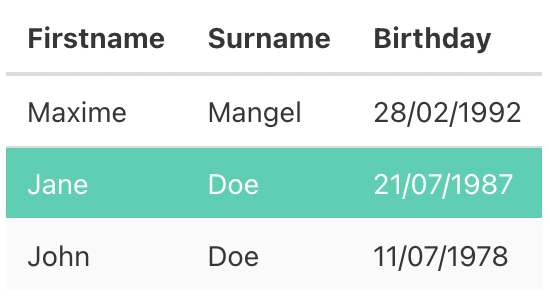
\includegraphics[width=0.5\textwidth]{02.Background/Fulma Table.png}
    \caption{Fulma Table Example}
    \label{fig:fulmatable}
\end{figure}


\subsection{Overview}
\begin{figure} [h]
    \centering
    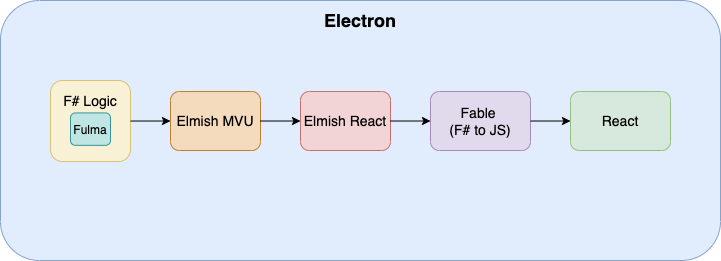
\includegraphics[width=\textwidth]{02.Background/Stack.png}
    \caption{An Overview of Issie's Technology Stack}
    \label{fig:techstack}
\end{figure}
We can bring the above sections together to get an overview of Issie's Technology Stack, which is presented in Figure \ref{fig:techstack}. The core logic of the Issie application is written in F\fsharp, with a structure which allows for adoption of the MVU architecture. Within the View function, using libraries like \codestyle{Fable.React} and \codestyle{Fulma}, HTML and React components can be specified. The \codestyle{Elmish} library provides the MVU framework and methods for bringing together the Model data structure, View function, and Update function. A virtual DOM is necessary for an MVU application because it allows the application to frequently re-render its state after each update in an efficient manner. Due to its reliable and performant implementation of a virtual DOM, the React framework is used for Issie. The library \codestyle{Elmish.React} handles the transition from the generic Elmish view to React, after which \codestyle{Fable} compiles all of this F\fsharp code to JavaScript for React to render. All of this runs within Electron, allowing Issie to run as a desktop application despite having the technology stack of a web app.

\section{Issie's UI} \label{sec:IssieUI}
\subsection{Overview and Evaluation}
In line with the core principles that state all features implemented in Issie should be \textbf{Obvious} and \textbf{Intuitive}, Issie's UI aims to be consistent and straightforward. Consistency in the UI helps constantly prove a user’s assumptions about the user interface right, creating a sense of control, familiarity, and reliability \cite{uiconsistency}. It also plays a crucial role in exposing all of the features of an application to the user -- this is because features which are accessed in an inconsistent manner may be missed or incorrectly understood by end users. The intuitive guidance provided by a consistent and straightforward UI means that students using Issie spend less time learning how to use it compared to other similar applications; at it's launch most students were able to get started within five minutes \cite{marco_diss}. With the limited amount of time in labs available, less time spent learning to use tools means more time spent on learning educational content.

Since its original release, more features have been added to Issie, such as the Waveform Simulator, with the UI being updated to accommodate these features. At the time of writing, the latest release version of Issie is version 3.0.0, released on 16th April 2022. Images of Issie's UI can be found in Appendix A. On launch, Issie gives the user the option to create a new project or open an existing one. A project consists of one \textbf{main} sheet, and any number of sub-sheets, which define reusable custom components. Figure \ref{fig:IssieSheetAnnotated} is an annotated screenshot of a sheet open in Issie. The UI can be split into the following sections, which are highlighted in different colours in Figure \ref{fig:IssieSheetAnnotated}.

\begin{itemize}
    \item[] \textbf{Traditional Menu Bar (Highlighted Red):} The traditional menu bar, consists of the "Edit" and "View" menus. It is not used to expose Issie's core features - instead, it is used to let the user do basic operations, such as zooming, copying and pasting etc. Many of these functions are duplicated through keyboard shortcuts or through the buttons in the bottom left of the sheet (undo, redo, copy, paste). The fact that Issie has two separate menus is a little strange, and it may be worth moving all functionality from the traditional menu bar to the top white menu bar. However, this is not an urgent cosmetic issue.
    \item[] \textbf{The Canvas:} The canvas is the central focus of the application - it is where the schematic is designed. Components are dragged onto the canvas, with red-dashed lines appearing to show when a component is aligned with a grid line. Components and connections on the canvas can be interacted with in many ways, such as hovering, clicking to select, and dragging to move.
    \item[] \textbf{Right Tabs Panel (Highlighted Green):} The panel on the right-hand side of the application provides the user with ways of (i) affecting the state of the canvas and (ii) gaining insight into the schematic itself. There are three tabs: the \textbf{Catalogue}, which lets users add new components to the canvas (users can hover on components for details); \textbf{Properties}, which lets users view and modify component properties like name and width, and \textbf{Simulation}, which opens the Step Simulator, giving users the option to start a simulation. Due to the Step Simulator requiring more display real-estate, the right panel widens when the Simulator tab is selected. When the Waveform Simulator is running, an additional fourth tab  appears in this section -- this makes the tab layout appear cramped.
    \item[] \textbf{Top Bar (Highlighted Blue):} In the first release of Issie, the white menu bar located at the top of the application contained controls to, (i) save the current sheet, (ii) Switch to another sheet in the open project, and (iii) Open another or create a new project. The filepath of the current project and sheet are also displayed. All of these elements were consistent - with the focus on interacting with files. A slight grievance with the "Project" and "Sheets" dropdown menus is that they are not closed by clicking elsewhere in the application, only by clicking on the menu again. Since then, an "Info" button has been added featuring information about Issie and a short user guide. While this is not necessarily consistent with the other elements in its vicinity, the top bar enables the "Info" button to have maximum visibility, something which a student requiring information may appreciate. One very inconsistent part of the UI is how the Waveform simulator is accessed. While most actions which analyse the schematic (e.g. Step Simulator) are accessed via the Right Tabs panel, the Waveform simulator is opened through a button on the top bar. This causes the previously unseen "WaveSim" tab to spawn in the right panel, and the panel boundary becomes draggable. The user can select the waveforms to view (Figure \ref{fig:IssieWSSel}) and then view the waveforms (\ref{fig:IssieWS}. The Waveform simulator's behaviour is inconsistent with that of the Step simulator:
    \begin{itemize}
        \item Step Simulator displayed in a wider, fixed-width panel. Waveform Simulator displayed with panel starting at regular width, but the panel can be manually resized by dragging.
        \item The user can start a simulation in the Simulation tab, and still interact with other tabs. This is not the case for the Waveform simulator, which locks the user in the WaveSim tab.
        \item Step Simulation started and ended with the same button, with a clear indication of how to end the simulation. There is no end/close button on the WaveSim tab when waveforms are being viewed. Instead, the user must press the "Edit List" button, which takes them back to the selection menu where there is a close button. This is very unintuitive.
    \end{itemize}
    \item[] \textbf{Buttons on bottom-left (Highlighted Yellow):} Undo, Redo, Copy, and Paste buttons. These are four common functions, and therefore it makes sense to have obvious and fast ways to access them. Useful to get started if the user is not familiar with keyboard shortcuts.
\end{itemize}

\subsection{Considerations when adding new features}
As discussed in the previous section, Issie's UI at time of launch was very intuitive and straightforward. However, when there are fewer features it is easier to condense the interfaces for them into a well structured and streamlined UI. The inconsistencies of the Waveform Simulator tell a cautionary tale of how new features can introduce impurities into an application's GUI. This project aims to add a whole new way of visualising logic (truth tables) to Issie, and given the saturated nature of the current UI, some redesigning may be necessary to accommodate all features.

\section{Combinational Logic Simulation in Issie} \label{sec:simulationbackground}
Currently in Issie, the users can gain an understanding of combinational logic by simulating it using the Step Simulator. Users provide values for each input to the logic, and can read the output almost instantly. This indicates high performance. Given that visualisation of combinational logic through truth tables is likely to require some form of combinational simulation, there is merit in exploring and understanding the implementation of the performant Step Simulator.

Figure \ref{fig:flowchartSim} provides an overview of Issie's process for building and running a Step Simulation. In this process, various checks must be performed; firstly the logic designed by the user must be verified to be syntactically correct, secondly the organisation of project files must be correct, and thirdly some Issie specific limitations (e.g. no cycles in combinational logic) must be enforced. Issie's simulation building process can be said to have three levels, with each level having an associated data structure which represents the schematic. These data structures are: the \textbf{Canvas State}, \textbf{Simulation Data/Error}, and a \textbf{Fast Simulation}. A set of checks are performed at each level, and only upon passing these checks can a schematic be transformed into the subsequent data structure.
If any of these checks fail due to an issue with the user's schematic, the simulation building process returns a \textit{SimulationError}, which tells the user what the error is and which components/connections are affected. A key takeaway from Figure \ref{fig:flowchartSim} is that the process of building a simulation is separate from the process of running it. During the \codestyle{FastSimulation} building process, the schematic is analysed, with components being placed into an appropriate order for combinational reduction. However, as the \codestyle{FastSimulation} data structure is mutable, the values of each input can be updated without having to rebuild the whole simulation. Therefore, the time taken simulating a different input combination is quite short, as only the reduction function has to be re-run to find the new outputs. 
This distinction between building a simulation and running it with different input values makes the existing Step Simulator an optimal choice for use in truth table generation, which will need to simulate multiple input combinations as fast as possible. 

\begin{figure}[h]
    \centering
    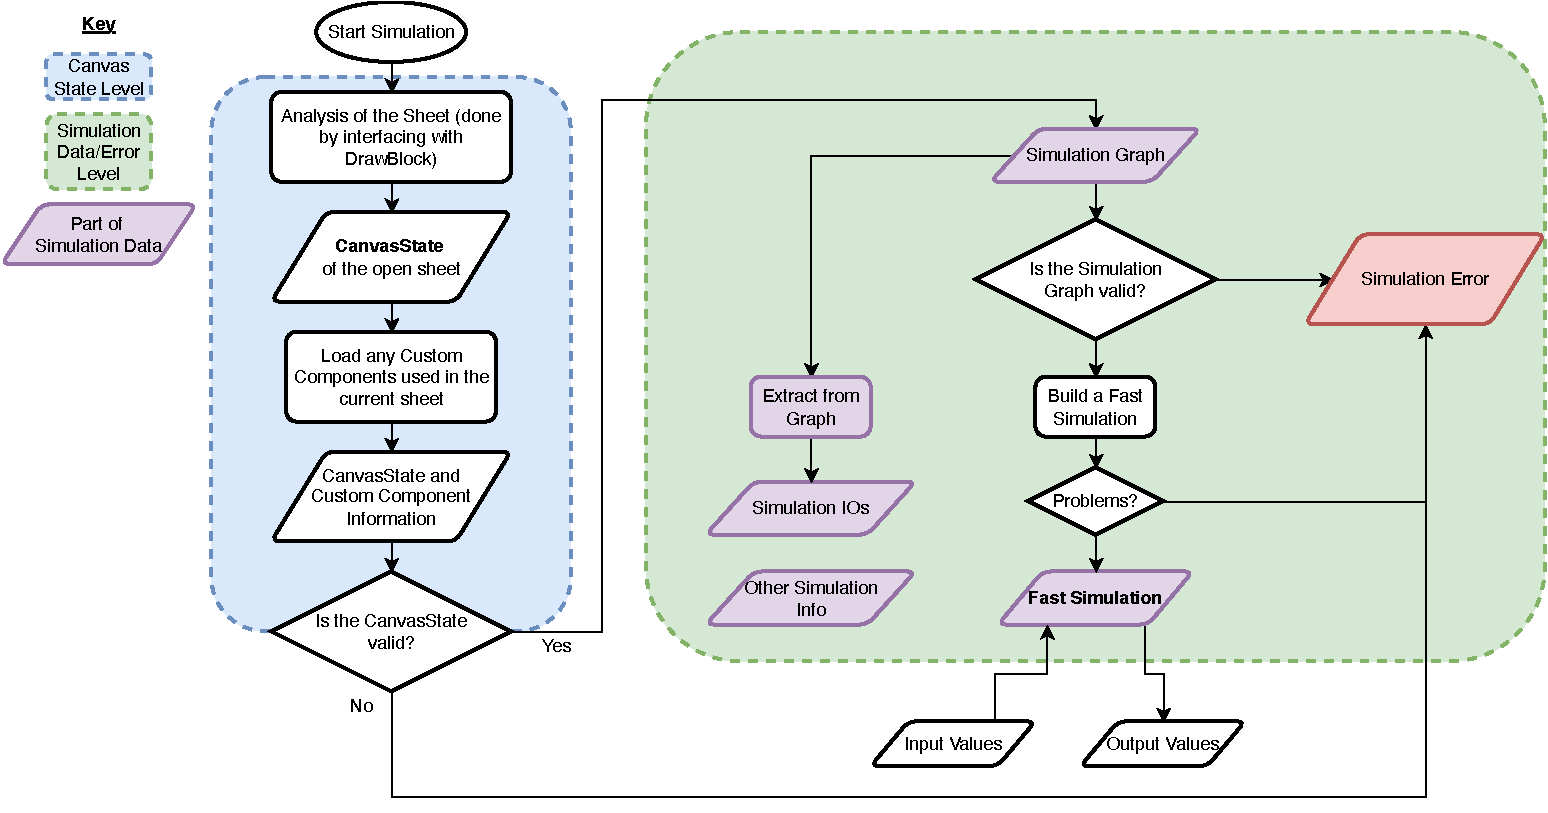
\includegraphics[width=\textwidth]{04.AnalysisDesign/IssieSim.pdf}
    \caption{An overview of Issie's Step Simulation}
    \label{fig:flowchartSim}
\end{figure}

\section{Effects of Application Performance on Users} \label{sec:perfeffects}
Interactivity is a key part of Issie, and one of the major contributors to perceived interactivity is the perceived responsiveness of an application \cite{interactiveWu}, which itself is often tied to application performance. Perceived responsiveness is relevant in systems where a user's "perceived control over the interaction process reflects their ability or confidence in performing related activities". Combining these findings with the cognitive theory of self-efficacy described in Section \ref{subsec:self_efficacy}, which proposes that academic performance is linked to perceived ability, indicates that perceived responsiveness is an important factor to consider when building an educational application. Robert Miller \cite{Miller1968ResponseTI} describes three classes of perceived responsiveness based on a computer's response time:
\begin{itemize}
    \item $\leq 100ms$: Perceived as instantaneous.
    \item $\leq 1s$: Noticeable but does not lose the user's attention.
    \item $\geq 10s$: Loses the user's attention.
\end{itemize}

Ideally, every interaction would be in the first class, however naturally certain tasks will take longer than others. In his paper, Miller investigates specific "Topics": examples of human-computer interaction, and examines the acceptable response time. A \textit{"Response to complex inquiry in tabular form"} (Topic 9) should return a complete response within 4 seconds, but a maximum delay of 2 seconds is preferred. This is particularly relevant to this project as it resembles the operation of calculating and presenting a Truth Table to the user. Therefore, it could be suggested that in order for the added Truth Table generation feature to have the maximum positive effect, generation should take less than 4 seconds in all cases, and ideally less than 2 seconds for simpler cases. By the same rationale, this time limit should also apply to complex operations on the truth table, such as reduction with Don't Cares or Algebra.
As mentioned in subsection \ref{subsec:educating_engineers}, engineers tend to be kinesthetic learners and therefore are likely to prefer tools which let them interactively experiment with what they are learning. Therefore, it can be proposed that increasing the responsiveness of Issie (which increases perceived interactivity), will lead to a better learning experience. 


\section{Agile Software Development}
Agile software development \cite{alma9955899676101591} is an iterative approach to software development, prioritising an "agile" response to changing requirements and user feedback. In Scrum, a popular Agile framework, the development team's plan is split into short \textit{sprints}: 1-4 week periods of work which deliver some "product", which is fully usable in its own right \cite{mepCW}. The high-level descriptions of the work are organised in a structured list called the \textit{backlog}. The hierarchy in the backlog is as follows \cite{backlog}:
\begin{itemize}
    \item \textbf{User Story:} Is a short, basic task which should not take too long to complete. An example would be a task to move the waveform simulator to the right tab, next to the step simulator.
    \item \textbf{Epic:} A large body of work which consists of multiple user stories. An example of an epic would be to implement truth table generation for a user selection of components.
    \item \textbf{Initiative:} Represent overarching goals of the software development project, consisting of multiple epics.
\end{itemize}

Over successive sprints, the number of stories in the backlog should reduce. There are regular meetings with the product owners, during which the development team \footnote{Usually there is an intermediary (Scrum Master) managing the organisation of the development team. However, given that Final Year Projects that improve Issie rarely interact with one another, this role is mostly redundant.} receives feedback which can then be acted upon. This may often add more work to the backlog. This cycle of continuous development aims to deliver working products which match user requirements on a frequent basis.
A survey \cite{CHOW2008961} of software projects managed in an Agile fashion found that "The practice of agile software engineering techniques "is a critical success factor that contributes to the successful agile software development projects in terms of Quality and Scope". This is also reflected by industry, where Agile approaches to software development have succeeded where more traditional linear Waterfall-esque approaches have failed \cite{mepCW}.

In the context of this project, the "product owner" is Dr Thomas Clarke, who oversees the overall development of Issie, while the "development team" consists of the author and other students.
\chapter{Requirements Capture} \label{chap:requirements}
\section{Requirements for Logic Visualisation}
\subsection*{Essential Requirements}
The improved version of Issie delivered by this project must be able to:
\begin{itemize}
    \item[\textbf{E1.1}] Analyse a schematic containing \textbf{only combinational logic} and display a standard numeric truth table for that sheet.
    \medskip
    \item[\textbf{E1.2}] Analyse part of a schematic selected by the user containing \textbf{only combinational logic} and display a standard numeric truth table for that selection.
    \begin{itemize}
        \item[\textbf{E1.2.1}] New inputs and/or outputs should be created temporarily (if necessary) to feed inputs and/or read outputs from the selected logic.
        \item[\textbf{E1.2.2}] It must be clear which newly generated inputs/outputs shown in the truth table correspond to inputs/outputs into the selected logic.
    \end{itemize}
    \medskip
    \item[\textbf{E1.3}] Have a truth table generating algorithm which can handle:
    \begin{itemize}
        \item[\textbf{E1.3.1}] Multi-bit inputs and outputs. Any temporary inputs/outputs created while generating a truth table for a selected logic block must have correct widths.
        \item[\textbf{E1.3.2}] Custom Components (sub-sheets), including when they are part of selections.
        \item[\textbf{E1.3.3}] Displaying inputs, outputs, and viewers.
    \end{itemize}
    \medskip
    \item[\textbf{E1.4}] Give users an option, when possible, to reduce the truth table based on patterns in the logic (e.g. Don't Cares).
    \medskip
    \item[\textbf{E1.5}] Give users the option to filter the truth table by fixing input or output values.
    \medskip
    \item[\textbf{\textbf{E1.6}}] Truth Tables must be displayed in a clear and easy to understand format, and features involving truth tables (e.g. filtering, reducing etc.) must be presented in an intuitive way.
    \item[\textbf{\textbf{E1.7}}] Truth Table generation and reduction must take no longer than 4 seconds.
    \item[\textbf{\textbf{E1.8}}] Graphical manipulation operations on the Truth Table, such as re-ordering rows, sorting etc. should appear instantaneous (i.e. take less than 100ms).
    \item[\textbf{E1.9}] Use the above features to give users a clearer insight into the digital logic on the schematic, or to further reinforce their existing understanding.
\end{itemize}

\subsection*{Desirable Features}
\begin{itemize}
    \item[\textbf{D1.1}] Generate and display algebraic truth tables.
    \begin{itemize}
        \item[\textbf{D1.1.1}] At minimum should at least support multiplexer and adder circuits.
        \item[\textbf{D1.1.2}] Preferably should have a rich set of algebraic operators with support for most circuits.
    \end{itemize}
    \medskip
    \item[\textbf{D1.2}] Provide an interactive truth table interface.
    \begin{itemize}
        \item[\textbf{D1.2.1}] Mousing over parts of the truth table could have effects on the schematic (e.g. annotations or highlighting).
        \item[\textbf{D1.2.2}] Users can rearrange order of columns/rows in the truth table.
        \item[\textbf{D1.2.3}] Users can sort the truth table in ascending and descending order.
    \end{itemize}
    \medskip
    \item[\textbf{D1.3}] Let the user access truth table related functionality without going through numerous steps \textbf{while} also keeping the number of buttons on the screen to a minimum to avoid cluttering the interface. 
    \medskip
    \item[\textbf{D1.4}] Extend truth table generation to sequential circuits in a similar way to the step simulator by allowing users to view the truth table at different clock ticks. When combined with the option to filter a truth table, this feature could be quite useful.
    \medskip
    \item[\textbf{D1.5}] Upon generation of a truth table for selected logic, display the selected logic as its own schematic including any temporarily generated inputs/outputs.
    \medskip
    \item[\textbf{D1.6}] Provide some kind of testbench functionality for combinational circuits, as truth tables are a complete definitive description of the behaviour of logic. Instructors could supply a testbench file containing the truth table for the correct solution, and Issie could determine the input combinations for which the user's code did not match the required output.
    \medskip
\end{itemize}

% \section{Requirements for Logic Input}
% \subsection*{Essential Requirements}
% \begin{itemize}
%     \item[\textbf{E2.1}] Generate a correct Issie Custom Component using a user-supplied truth table.
%     \medskip
%     \item[\textbf{E2.2}] Users should be able to supply a truth table through Issie's GUI, or through a specified file.
% \end{itemize}

% \subsection*{Desirable Features}
% \begin{itemize}
%     \item[\textbf{D2.1}] Generate a correct Issie schematic using a user-supplied truth table, with the option for SOP and POS interpretations.
%     \begin{itemize}
%         \item[\textbf{D2.1.1}] Components in the generated schematic must be clearly spaced and laid out in a reasonable form.
%         \item[\textbf{D2.1.2}] Use intelligent analysis or Boolean Algebra to generate a schematic using as many components in Issie's catalogue as possible.
%     \end{itemize}
%     \medskip
%     \item[\textbf{D2.2}] If intelligent analysis is implemented, then use the same mechanism to simplify existing schematics.
% \end{itemize}

\section{Software/Documentation Quality Requirements}
\subsection*{Essential requirements}
\begin{itemize}
    \item[\textbf{E3.1}] Deliver performant, working, bug-free code which adheres to Issie's code guidelines and other principles such as "MVU-ness".
    \medskip
    \item[\textbf{E3.2}] Write comments in the delivered code which adequately explain it such that it may be worked on in the future by other developers. 
    \medskip
    \item[\textbf{E3.3}] Provide any other necessary documentation
\end{itemize}

\subsection*{Desired features}
\begin{itemize}
    \item[\textbf{D3.1}] Deliver a tweaked, or possibly partially redesigned UI which exposes all Issie features in a straightforward and intuitive way to the user, with a focus on extensibility (i.e. can the UI accommodate for future extensions to Issie?)
    \medskip
    \item[\textbf{D3.2}] Update the Issie website with information about any newly added features.
\end{itemize}
\chapter{Analysis and Design}
This chapter describes all the changes and additions made to Issie by this project, as well as organisational decisions. Additionally, the rationale behind these changes, including analysis of high-level methods, will be explained. 
\section{Approach towards Software Development}
Features were added to Issie using an incremental and Agile approach \cite{Voorhees2020}.
The incremental approach seeks to write code through a repeated cycle of three steps: (1) Analysis and Design, (2) Writing Code, and (3) Testing. A basic task/requirement is  broken into several parts - with each of these parts being written as an individual function \footnote{"individual function" does not refer to a single F\fsharp function, but to a top-level function which uses groups of helper and sub-functions}. Each function is tested both as a unit and when integrated into the codebase. All of these different parts build upon one another and come together to deliver the desired functionality. One caveat of the incremental approach is that the intermediate versions of the app are incomplete and therefore not suitable for any kind of release or proper demonstration. This can make it difficult to get proper feedback on the state of the application as a whole. This was acceptable within short time-frames, but not for long-term software development over the course of the project. For that case, the Agile approach was considered. Small features, represented as a short sequence of stories, were built using the aforementioned incremental approach during sprints. Upon completion of each feature, it could be considered that a new "product" (slightly improved version of Issie) was delivered. During each project meeting, feedback was obtained on the work completed, and any necessary adjustments will spawned new user stories. Agile is generally used in continuous software development projects; however, due to the constraints of a Final Year Project: deadlines, need for planning and report writing, a pure Agile approach was not deemed not suitable. Instead, a hybrid approach was pursued, one which embodies Agile principles while still working within a plan-based framework. During the planning phase, the backlog of user stories was intelligently structured such that epics were ordered by importance to the project, and stories within the epics were structured such that features would be added incrementally.

\section{Technology Stack}
This project does not make any deviations from Issie's existing technology stack, described in Section \ref{sec:techstack}. The F\fsharp application code is compiled to JavaScript using the Fable compiler, and is run as a web app in a desktop environment using Electron. The user interface is powered by React and the MVU architecture, brought to the F\fsharp ecosystem by the \codestyle{Fable.React} and \codestyle{Elmish} libraries. New files added to the Issie codebase by this project are split between two existing directories in the \textit{Renderer} project. Files which implement features related to actual truth table generation and reduction are placed in the \textit{Simulator} directory, while files which implement the UI are placed in the \textit{UI} directory. 

% \section{Overview of Added Features}
% This section describes all the changes and additions made to Issie by this project. In subsequent sections in this chapter, the rationale behind these changes, including analysis of high-level methods, will be explained. Finally, in the Implementation chapter, the details of how these features were implemented will be explained. 

\section{Top Level UI Changes}
The top-level UI of the application has been changed to accommodate truth tables. As a result of this, the way the waveform simulator is accessed has been changed as well. In prior versions of Issie, the right tab section had three options: \textbf{Catalogue} for adding new components, \textbf{Properties} for changing component properties, and \textbf{Simulation} for launching the Step Simulator. When applicable, Waveform Simulator could be accessed by clicking a button in the top bar, which would temporarily create an extra tab in the right section. Given that most interactions related to modifying or gaining insight into the schematic were done through the right section tabs, the decision was made for the truth table to be displayed there. The large amount of space needed to display a truth tables and related functionality warranted a separate tab for truth tables. However, this approach posed some potential problems. During the earlier evaluation of Issie, it was found that the method of accessing the waveform simulator was inconsistent, and that the waveform simulator should ideally have it's own permanent tab too. Therefore, the total number of tabs would increase from three to five, resulting in a cramped layout. 
The updated version of Issie delivered by this project solved this problem by grouping all circuit simulation activity under one tab. The third tab in the right section has been re-named to \textbf{Simulations} and features three further sub-tabs, each for the Step Simulator, Truth Table generator, and Waveform Simulator respectively. This can be seen in Figure \ref{fig:issieview}, where the \textbf{Truth Table} sub-tab is open. 
From this tab, the user can choose to generate a truth table for the whole sheet. Additionally, if a correct configuration of components is selected, a second option to generate a truth table for the selected configuration is also shown to the user. As with the Waveform Simulator, when the Truth Table tab is open, the dividerbar can be dragged to resize the right section. Previously, there was a bug where, if the right section was scrollable, the dividerbar height did not dynamically resize. This bug was fixed by this project.
\begin{figure}[h]
    \centering
    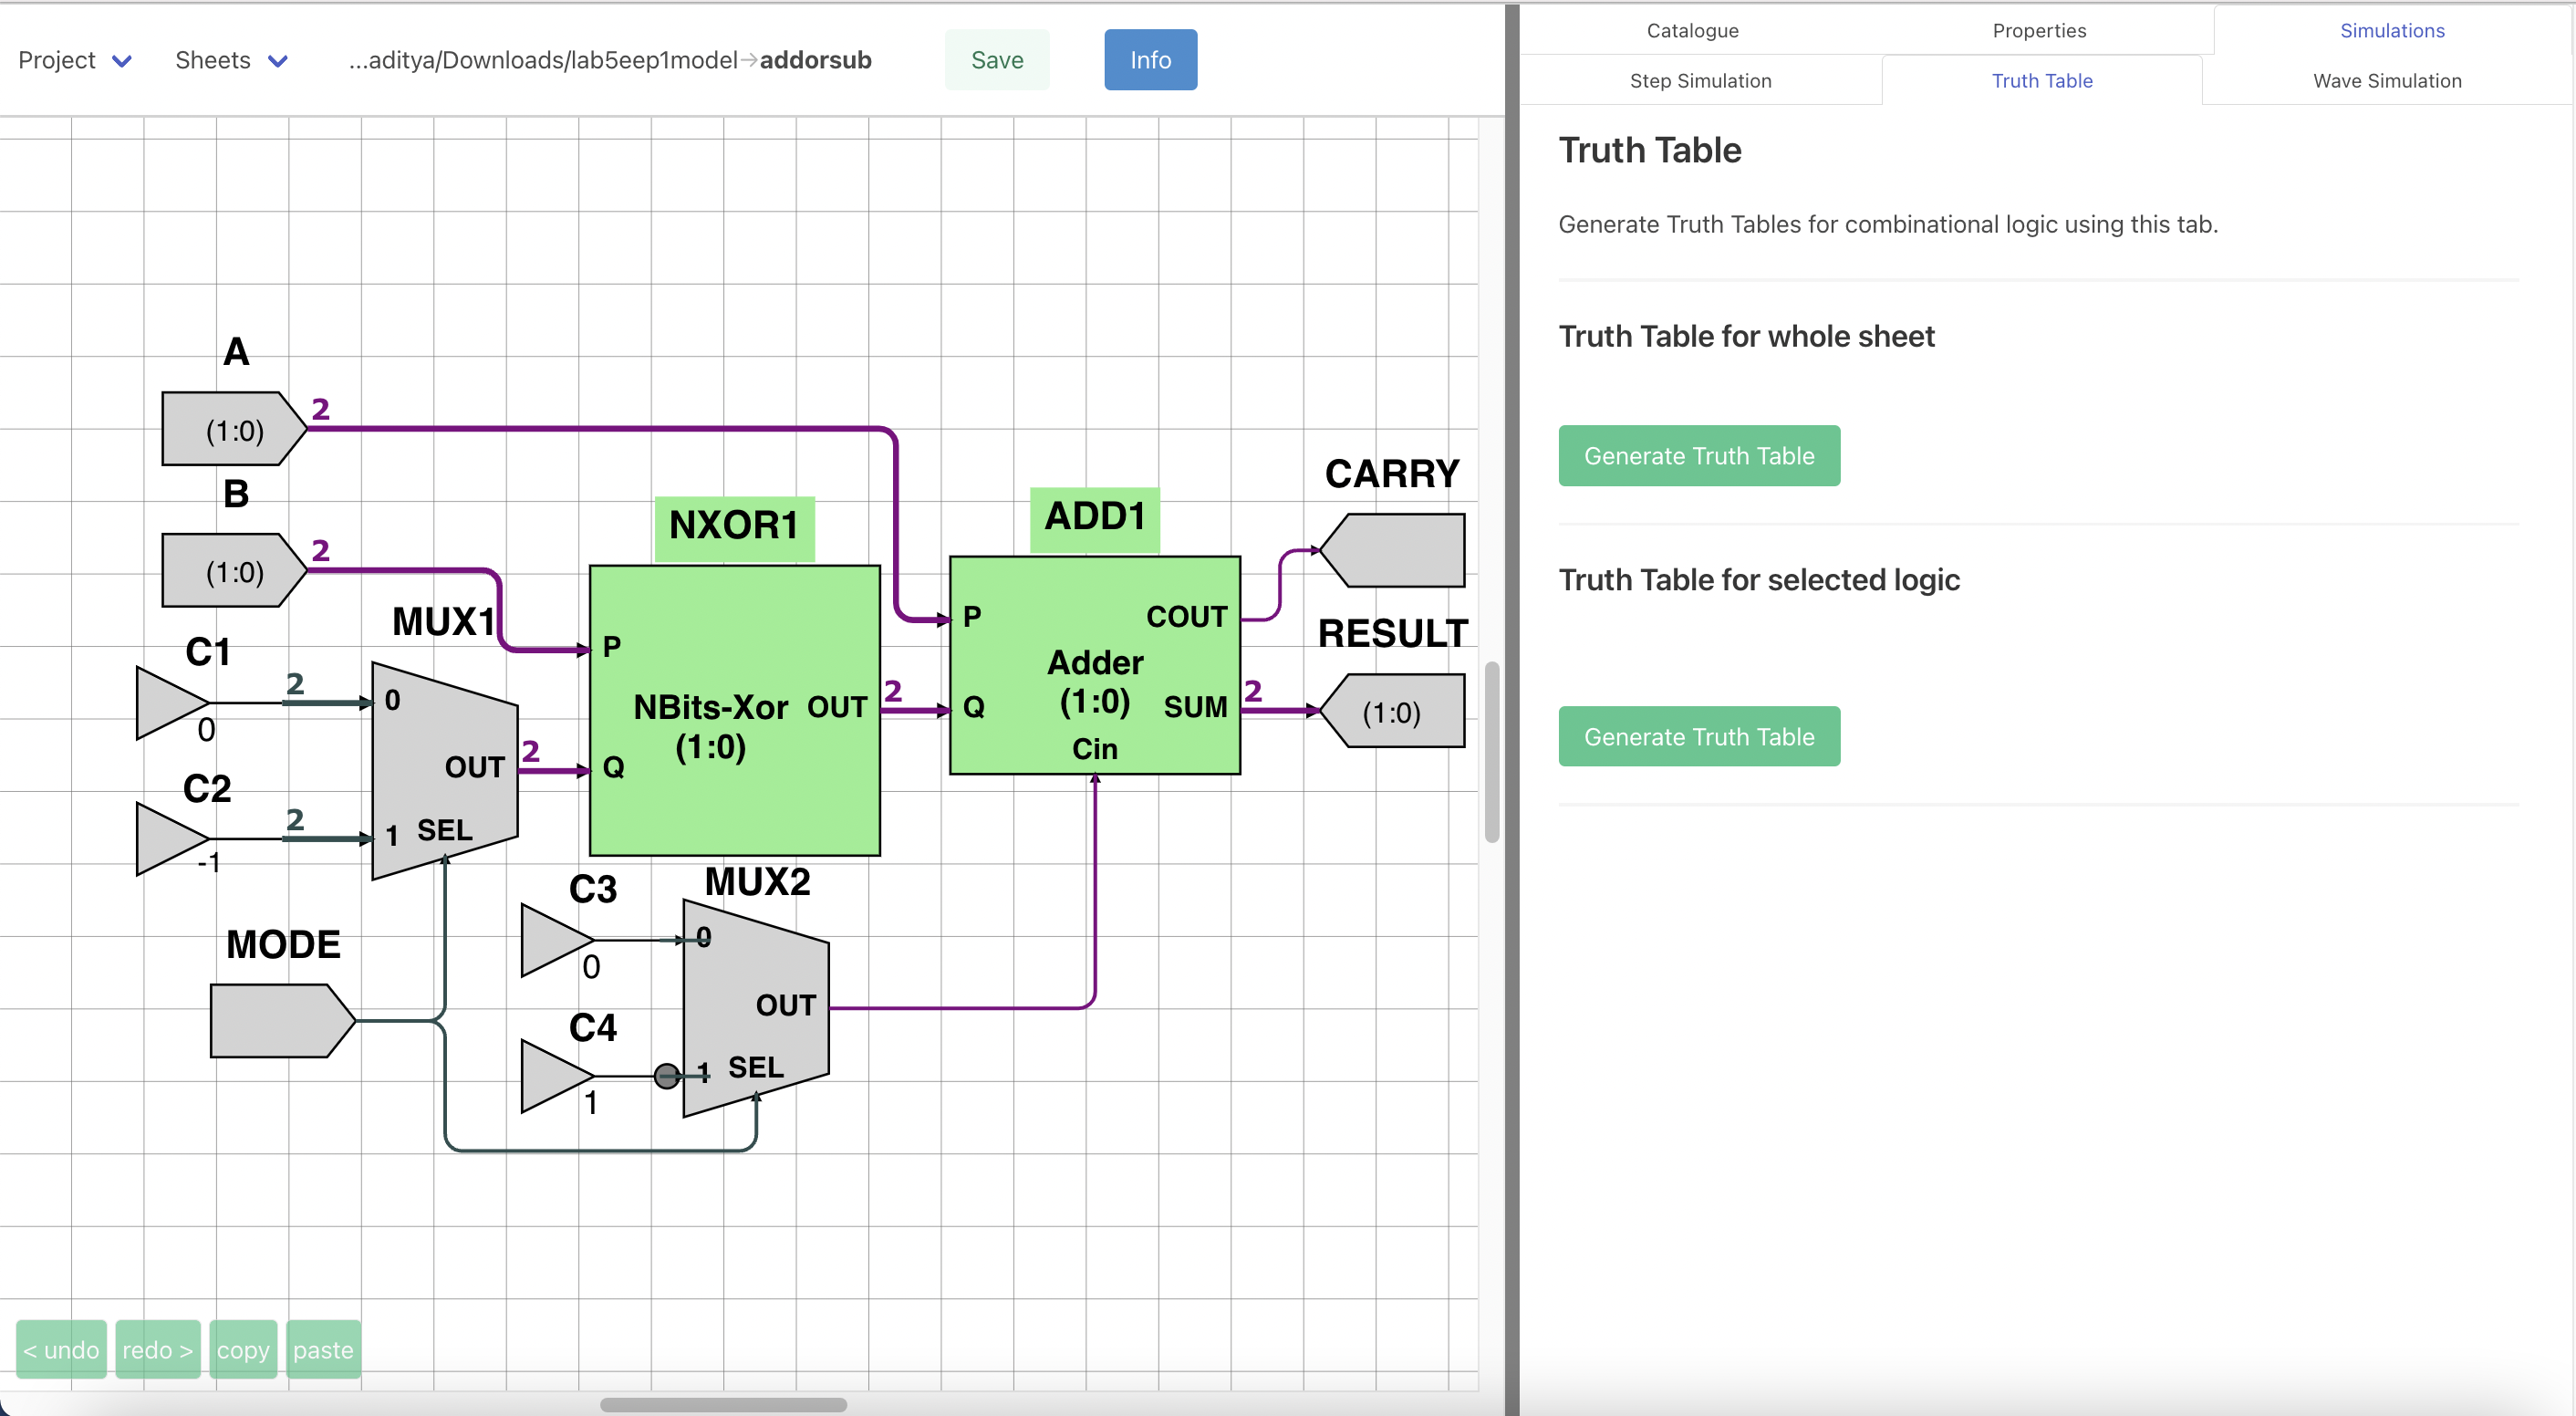
\includegraphics[width=\textwidth]{04.AnalysisDesign/Issieview.png}
    \caption{View of Issie's updated Top-Level UI}
    \label{fig:issieview}
\end{figure}

\section{Generating Numeric Truth Tables} \label{sec:analysis_ttGen}
The user can generate a truth table by clicking on the \textit{Generate Truth Table} button. Like the  \textit{Star Simulation} button in the Step Simulator, this button provides feedback on the correctness of the canvas to the user through colours. A green button indicates a correct canvas which can be used to generate a truth table. If there are issues with the schematic, the button will instead be yellow, and clicking it will inform the user of the nature of the error via an error message and highlighting the erroneous component. Finally, the button can also be a faded green; this indicates that while the schematic is correct, it is unsuitable for truth table generation as it contains sequential logic. This is done to maintain consistency with the Waveform Simulator button, which becomes faded when there are no sequential components.

When the user generates a truth table, a numeric truth table is generated at first. Due to performance reasons, which will be discussed later, Issie will only generate up to the first 1024 rows in a truth table. In cases where the truth table should have been larger than this limit, it is considered \textit{truncated}. The user is warned of this through a yellow coloured popup with the following message: \textit{"The Truth Table has been truncated to 1024 input combinations. Not all rows may be shown. Please use more restrictive input constraints to avoid truncation"}. Once a truth table is generated, the user can interact with it in numerous ways through the user interface, transforming and regenerating it as necessary. Figure \ref{fig:tttab} shows two views of the Truth Table tab, which contains a menu with collapsible sections. The compact view (Figure \ref{fig:compact}) is the default, with all sections other than the one displaying the truth table, reduction operations, and base selector being collapsed. The other sections can be expanded to reveal additional functionality; Figure \ref{fig:expand} shows the view of the Truth Table tab when all sections are expanded. The tab section is also scrollable.

Figure \ref{fig:ttGen} shows a high-level overview of the truth table generation process. This process will be covered in more detail in the Implementation chapter, but the overall process can be summarised into three phases: building the simulation, finding the input combinations which make up the left-hand side of the the truth table (Input Space), and simulating each combination in the input space to build the truth table. Decisions had to be made on how to generate the input space, as well as how to simulate each input combination.

\begin{figure}[h]
     \centering
     \begin{subfigure}[b]{0.48\textwidth}
         \centering
         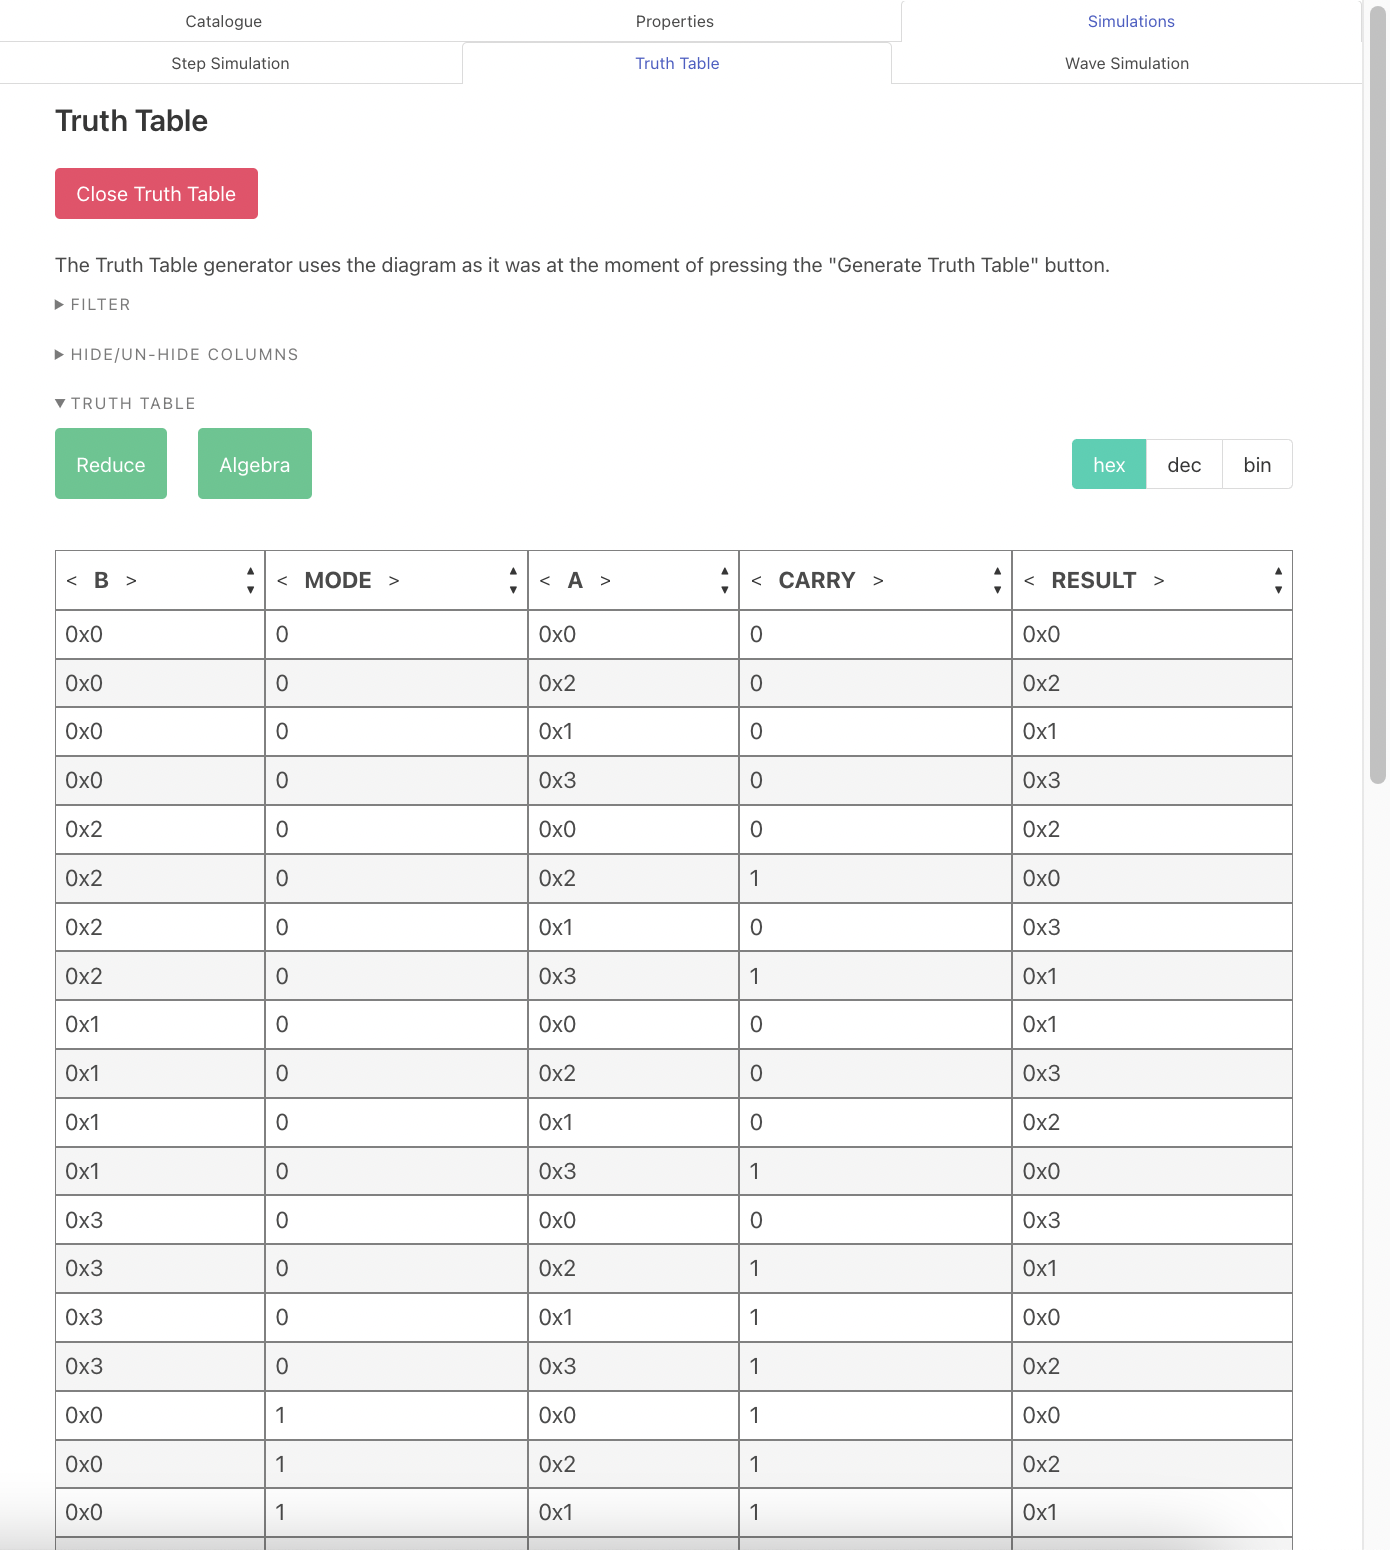
\includegraphics[width=\textwidth]{04.AnalysisDesign/compact.png}
         \caption{Compact View}
         \label{fig:compact}
     \end{subfigure}
     \begin{subfigure}[b]{0.48\textwidth}
         \centering
         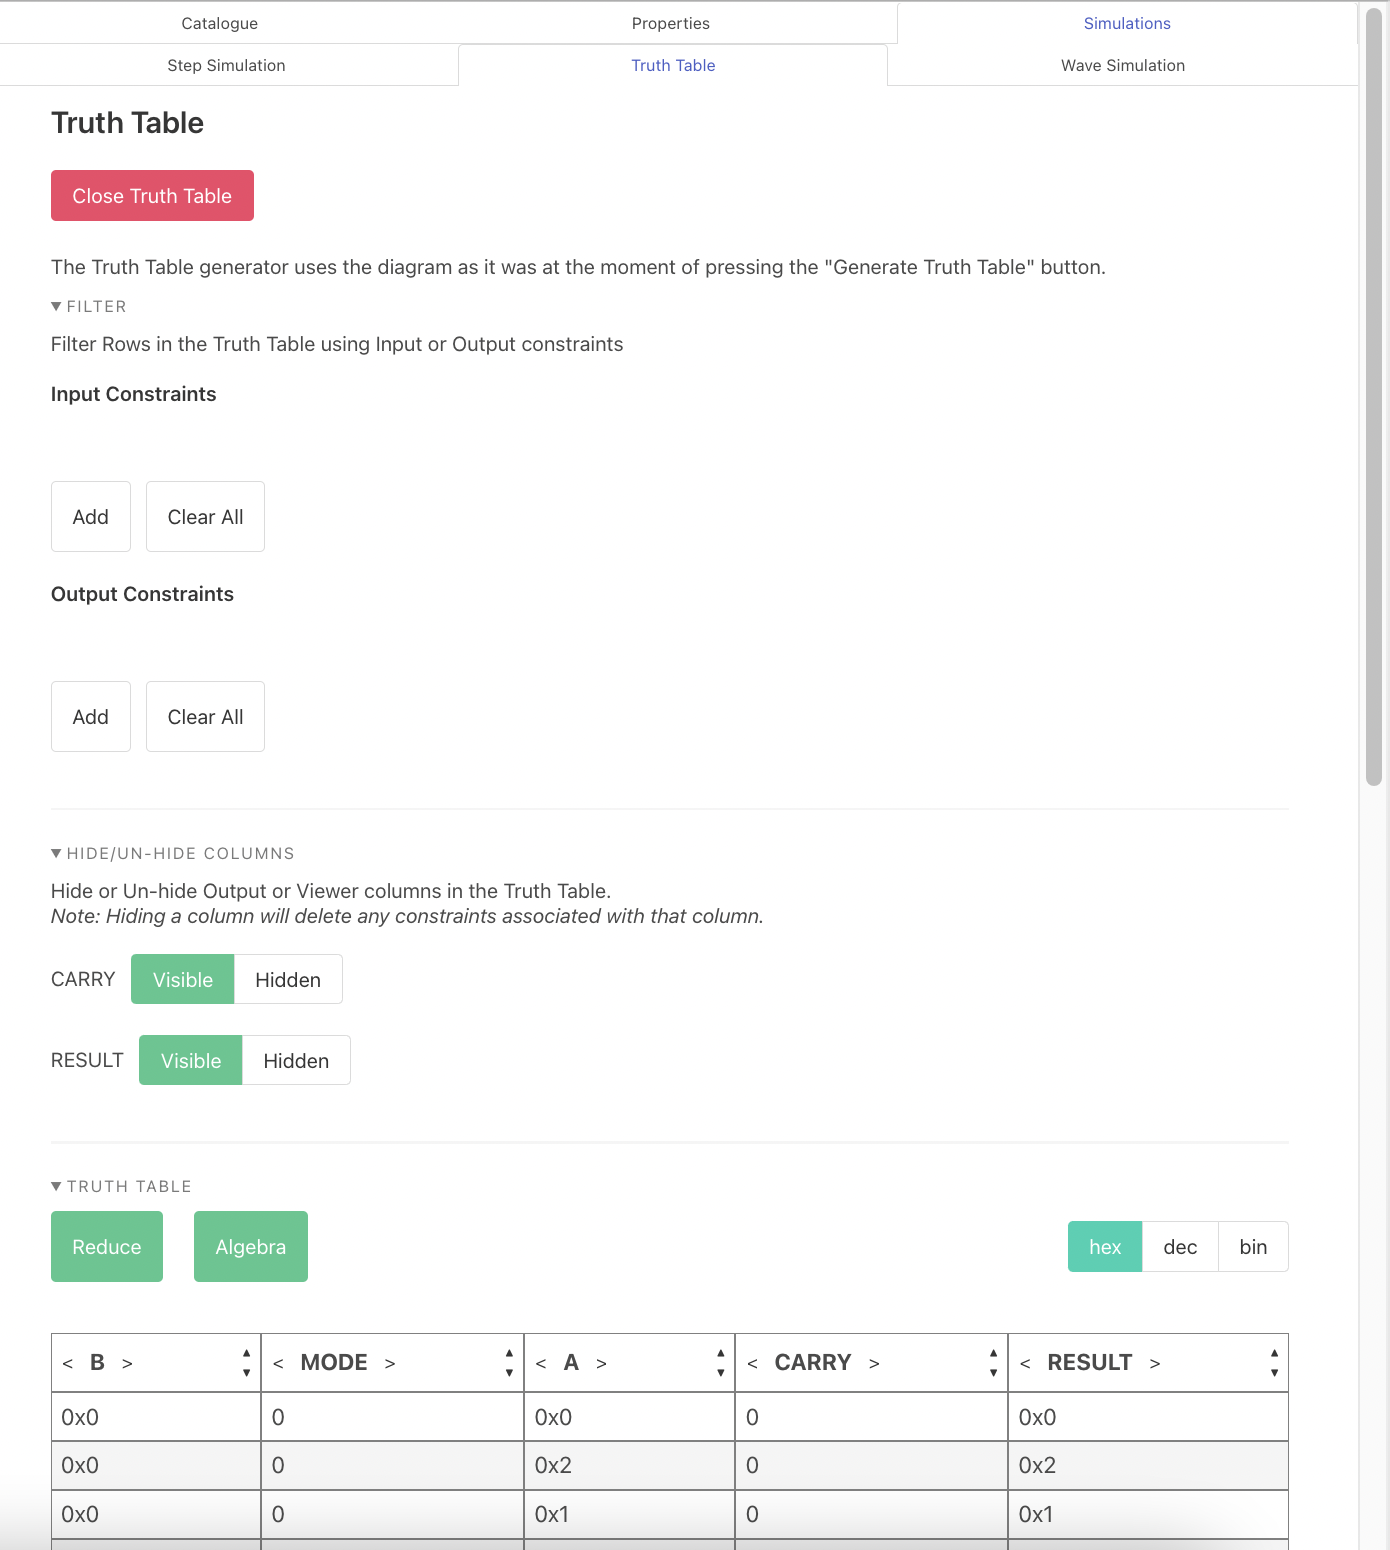
\includegraphics[width=\textwidth]{04.AnalysisDesign/expanded.png}
         \caption{Expanded View}
         \label{fig:expand}
     \end{subfigure}
        \caption{Contents of Truth Table tab after a truth table has been generated}
        \label{fig:tttab}
\end{figure}

A decision also had to be made regarding the handling of multi-bit IOs.
In Issie, inputs to combinational logic can be multi-bit (width > 1), and propagate through the logic via multi-bit buses. Two possible approaches for handling these multi-bit inputs were considered. The first option was to split a multi-bit input into its constituent bits in the truth table; this aligns more closely with the actual hardware implementation of the logic \cite{muxtables}, where component ports only accept a single-bit signal. However, this is not user-friendly at all - for example a 32 bit bus would be split into 32 different inputs. This would massively increase the number of columns in the truth table, impacting the utility of the truth table as an aid. Furthermore, splitting inputs and outputs into separate bits would obscure certain relationships, such as those of arithmetic circuits. Instead, the decision was made to represent each multi-bit input/output as one column in the truth table, with the value shown in hexadecimal format by default. The user can choose between hexadecimal, decimal, and binary representations.

\subsection{Decision to re-use Step Simulation Code}
At its core, generating a complete numeric truth table is a brute-force process. Each possible combination of input values must be simulated to calculate the corresponding output values, and the relationship should be recorded in the table. 
Given that Issie already features a performant and reliable simulator (step simulator) for calculating the outputs of combinational logic, the decision was made to use as much of its implementation as possible. This approach has many advantages:
\begin{itemize}
    \item The existing step simulator has been extensively tested by end-users, meaning that its implementation is most likely bug-free. By using it, it will reduce the chance of the new feature introducing new bugs.
    \item In most cases, reusing existing code is much faster than writing new code from scratch. Not only is time saved on writing new code, but the amount of time spent debugging is also reduced.
    \item Reusing existing code will help keep the overall size of the codebase small. Not only does this help future programmers who work on the project by reducing how much they have to understand, but it also means that any future improvements made to the simulation code are also improvements to Truth Table generation.
\end{itemize}

% Figure \ref{fig:flowchartSim} provides an overview of Issie's process for building and running a Step Simulation. In this process, various checks must be performed; firstly the logic designed by the user must be verified to be syntactically correct, secondly the organisation of project files must be correct, and thirdly some Issie specific limitations (e.g. no cycles in combinational logic) must be enforced. Issie's simulation building process can be said to have three levels, with each level having an associated data structure which represents schematic. These data structures are: the \textbf{Canvas State}, \textbf{Simulation Data/Error}, and a \textbf{Fast Simulation}. A set of checks are performed at each level, and only upon passing these checks can a schematic be transformed to the subsequent data structure.
% If any of these checks fail due to an issue with the user's schematic, the simulation building process returns a \textit{SimulationError}, which tells the user what the error is and which components/connections are affected. A key takeaway from Figure \ref{fig:flowchartSim} is that the process of building a simulation is separate to the process of running it. During the \codestyle{FastSimulation} building process, the schematic is analysed, with components being placed into an appropriate order for combinational reduction. However, as the \codestyle{FastSimulation} data structure is mutable, the values of each input can be updated without having to rebuild the whole simulation. Therefore, the time taken simulating a different input combination is quite short, as only the reduction function has to be re-run to find the new outputs. 
% This distinction between building a simulation and running it with different input values makes the existing Step Simulator an optimal choice for use in truth table generation, which will need to simulate multiple input combinations as fast as possible. 




\begin{figure}[h]
    \centering
    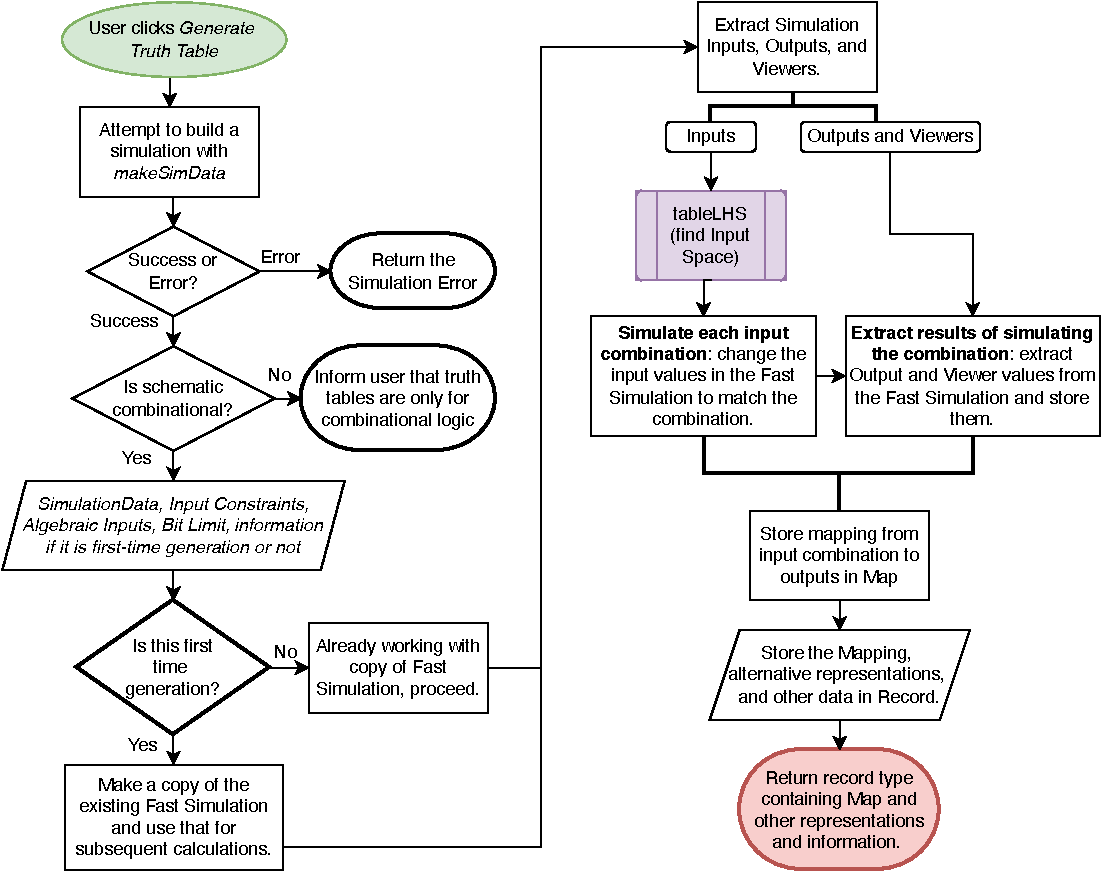
\includegraphics[width=0.8\textwidth]{04.AnalysisDesign/ttGen.pdf}
    \caption{High-Level view of Truth Table Generation}
    \label{fig:ttGen}
\end{figure}

% \begin{figure}[h]
%     \centering
%     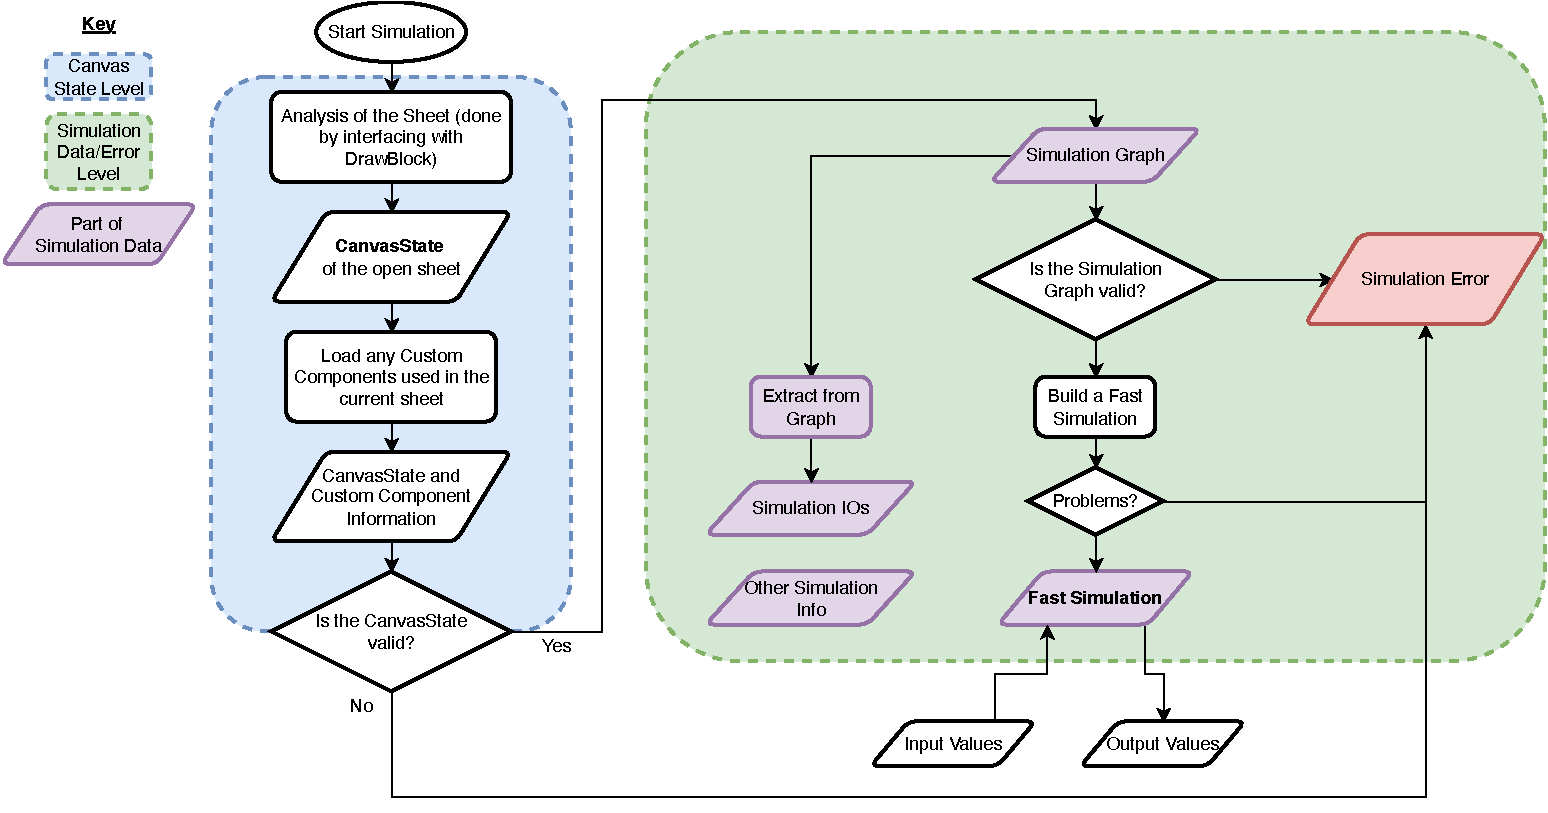
\includegraphics[width=\textwidth]{04.AnalysisDesign/IssieSim.pdf}
%     \caption{An overview of Issie's Step Simulation}
%     \label{fig:flowchartSim}
% \end{figure}

\subsection{Evolution of the Input Space Generation Algorithm} \label{subsec:evolutionofinputspace}
The process of calculating the input space, highlighted in purple in Figure \ref{fig:ttGen}, had two versions. The change from the first to the second version affected the overall structuring of operations on truth tables in the application. Initially, the entire input space was calculated and simulated. This would result in a very large, exhaustive truth table -- one which contained every possible input and output combination. The user would haven been able to reduce this truth table by filtering the table or using Don't Care Reduction. However, several issues arose with this approach, with the most crucial being that of performance. 

For a truth table with $n$ inputs ($x_1 .. x_n$), each of width $w$, ($w_1 .. w_n$), the number of rows in the truth table is given by the sum of all widths raised to the power of 2, as shown in Equation \ref{equ:rowcount}. For example, a schematic with three inputs, with widths: $w_1 = 1, w_2 = 2, w_3 = 3$ would result in a truth table with 64 rows. This sum-of-widths formula is derived from the idea that if we define a set $S_i$ as the set of all possible input combinations for input $x_i$, the left-hand side of a truth table is the \textbf{Cartesian Product} of all sets from $S_1$ to $S_n$. This project defines the left-hand side of the truth table as the \textbf{input space} of the truth table, and the right-hand side as the corresponding \textbf{output space}.
\begin{equation} \label{equ:rowcount}
    \textrm{Row Count} = \prod_{i=1}^{n} 2^{w_i} = \prod_{i=1}^{n} S_i = 2^ {\left( \sum_{i=1}^{n} w_i \right)}
\end{equation}

The complexity of finding the Cartesian product of multiple sets is an exponential function of the number of sets. For example, the complexity of finding the Cartesian product of $n$ sets, each of size $s$, would be $O(s^n)$. The size of each set is dependent on the width of the input; Issie does not limit input widths, meaning that the size of the sets may also be very large. For example, a single 16-bit input has 65536 unique values, and combining this with a second 16-bit input yields an input space of $2^{32}$ combinations (over 4 billion). Simulating this large number of combinations and storing the result takes upwards of 20 seconds, violating essential requirement \textbf{E1.7}. Additionally, a sufficiently large input space could cause the system to run out of memory and crash, which is unacceptable. Along with the practical issues with the generation of the complete truth table, it can also be argued that a very large complete truth table is not useful to the user. According to the Atkinson-Shiffrin memory model described in Section \ref{subsec:memmodels}, external stimuli only stay in the sensory register for 0.5 seconds prior to decaying. A large number of rows is likely to overload the sensory register, meaning that it is likely that the information will not pass to short term memory unless the the user slows down and processes each row one-by-one. Even if this were the case, a truth table with a large number of rows would take over 30 seconds for the user to read and process. Given that short term memory decays in 30 seconds, this means that the user will likely have forgotten the first row by the time they finish reading the last one. Therefore, the method of generating and simulating the entire input space to create an exhaustive truth table was deemed unfit.

As a result, the decision was made to \textbf{truncate the truth table}; generate and simulate only part of the input space. The current limit is 1024 rows. Considering that users would only be able to focus on a small subset of rows at a time, and would likely reduce the size of the table anyways, this approach would sacrifice very little for a significant gain. However, any subsequent operations, such as filtering and reduction, would take place on the truncated table, which does not contain all of the necessary data. The nature of these issues, as well as the steps taken to mitigate them are:

\begin{itemize}
    \item[] \textbf{Issue 1}: Input constraints will be applied to the truncated table, so user may not see a full representation of the relationships for the case they enter. For example, consider the input $X$ which has a width of 8 bits (so values range from 0 to 255), but due to truncation, only rows with values of $X$ up to 31 are present. If the user applies the input constraint $X = 32$ to the table, an empty table will be returned as no rows which fulfil this condition exist in the truncated table.
    \item[] \textbf{Solution 1}: Apply input constraints during truth table generation. This is achieved by using the constraints to determine a tighter input space, and then simulating that. Giving users a way to choose which inputs contribute more to the input space (they can fix certain inputs and let others vary within bounds) allows them to interactively generate truth tables that deliver the most information to them.
    \item [] \textbf{Issue 2}: Output constraints will be applied to the truncated table, which is missing many rows. Due to this, the result of applying the output constraints will include all rows which match the condition.
    \item [] \textbf{Solution 2}: Unfortunately there is not much that can be done to combat this issue alone other than warn the user that they are looking at incomplete results. However, if the user is able to use input constraints to sufficiently reduce the input space first, output constraints could help filter the table further.
    \item [] \textbf{Issue 3}: Don't Care Reduction will occur on the truncated table, which does not fully represent the logical function performed by the circuit. This could result in incorrect relationships being inferred by the reduction algorithm.
    \item [] \textbf{Solution 3} Much like with output constraints, there is no perfect solution as relationships for reduction are inferred from the truth table. Don't Care reduction is therefore limited to smaller schematics which do not produce truncated truth tables. The user is instead guided towards reducing truth tables for larger schematics with \textbf{Algebraic Reduction}.
\end{itemize}

Implementing Solution 1 required a new method of generating the input space. The new method needed to know which sub-sets of the input space it could and could not generate before it actually generated it using the Cartesian product method. Further details of the workings and implementation of this method can be found in the Implementation chapter.

\section{Generating Truth Tables for a partial selections}
The motivation behind Requirement \textbf{E1.2} is that a large schematic with lots of components will often contain smaller blocks of logic within it. These blocks may be defined Custom Components, or simply be a collection of gates in one corner of the canvas. Either way, there is value in the user being able to isolate these blocks and learn about the combinational logic implemented by them. Such functionality would also allow users to take a divide-and-conquer approach to debugging logical errors - individual blocks could be inspected to ascertain if they had been implemented correctly. 

A challenge with generating a truth table from part of a canvas is that Issie has no existing method for simulating part of a canvas. When working with a whole sheet, the inputs and outputs are well-defined; sheets where any ports aren't connected to inputs/outputs throw \textit{Simulation Errors}. In contrast, a partial selection from a sheet will rarely contain all inputs and outputs. Two methods were considered for simulating the selected logic to generate a truth table, with the latter being chosen.
\begin{enumerate}
    \item \textbf{Extracting the Fast Simulation and feeding values into specific wires}. This method would have involved creating a Fast Simulation for the whole sheet as usual, but then manually changing values in component arrays and seeing how those changes propagated through to the output connections of the selected logic. While this method seemed fit initially, several issues were found after some analysis. The Fast Simulation would be built for the whole sheet, meaning that an error elsewhere on the canvas would stop the selected logic from being simulated. Custom Components would also be harder to manage as the Fast Simulation datatype flattens the design, meaning that all nested logic in Custom Components would be expanded out. The new logic would also be quite different from the truth table generation logic for whole sheets - this is not ideal for future code maintenance purposes.
    \item \textbf{Intelligently building and correcting a new Canvas}. Following the highlighting of the issues with the first approach, an alternative approach was put forward. Rather than attempting to work with the complicated Fast Simulation data structure, it instead aims to use as much of the existing code as possible by treating the selected logic as a separate instance of a Canvas State and trying to simulate it using the same method as simulating a whole canvas. The main difference between simulating a whole sheet and simulating selected logic is the lack of guaranteed input and output components. This is overcome by finding which ports/connections are inputs/outputs for the selected logic, then intelligently adding 'phantom' input/output components to the canvas in a process called Canvas Correction. Once a corrected canvas corresponding to the selected logic is created, the logic used for generating and viewing a Truth Table for a whole sheet can be reused.
\end{enumerate}

The method implemented by this project first sanity-checks the part of the sheet the user has selected. Following this, the canvas correction algorithm adds new Input and Output components to the partial selection to transform it into a valid Issie schematic. The existing truth table generation process can then continue using this valid schematic.

\section{Filtering with Constraints}
Once a truth table has been generated, it can be filtered using constraints; these can be equality or inequality constraints. Equality constraints on an input or output (IO) are of the form $IO = value$, where the truth table is filtered such that only rows where the input or output (IO) is equal to the given value are shown. Inequality constraints are of the form $LowerBound \leq IO \leq UpperBound$; the filtered truth table will only contain rows where the IO is between the lower and upper bounds (inclusive). Due to reasons that will be discussed further in this chapter, applying input constraints will re-generate the table, while output constraints will only filter the existing table. 
Constraints are added through a popup window as shown in Figure \ref{fig:addconstraint}. Issie validates all constraints in real time; the user is prevented from entering an invalid constraint and is told the why it is invalid. This can be seen at the bottom of Figure \ref{fig:addconstraint}, where the message informs the user of the issue with the constraint they are trying to add. This approach has two major advantages. Firstly, from a system design perspective, the logic which applies the constraints can trust that all the constraints are well-formed and do not conflict with one another, maintaining robustness. Therefore error handling for constraints need not be implemented in these sections. Secondly, from a user experience perspective, this approach is more obvious and intuitive, aligning it with Issie's core principles. The issue with the user input (invalidity of the constraint) is addressed at the moment it happens, making it clear to the user exactly what has gone wrong. This is far more clear than propagating the error to the user later on in the process.
Once added, the constraint will appear as a small tag in the Filter section -- the constraint can be deleted by clicking the cross on the tag; alternatively all input or output constraints can be cleared by clicking the \textit{Clear All} button for each respective group.
\subsection{Constraint Validation Rules}
\begin{enumerate}
    \item All entered values must be valid numbers -- numbers can be entered in decimal, hex (\codestyle{0x}), or binary (\codestyle{0b}) form.
    \item All entered values must not exceed the width of the IO, with checks also implemented for negative numbers (e.g. cannot enter 9 or -6 for a 3-bit IO).
    \item Constraints must be unique; the entered constraint must not already exist.
    \item Constraints must not overlap. For example, if a constraint $X=5$ exists, the constraint $4 \leq X \leq 7$ cannot be added (and vice versa).
    \item For inequality constraints, the upper bound must be greater than the lower bound. This check is always performed using the unsigned representation of the number entered.
\end{enumerate}

\begin{figure}[h]
     \centering
     \begin{subfigure}[b]{0.4\textwidth}
         \centering
         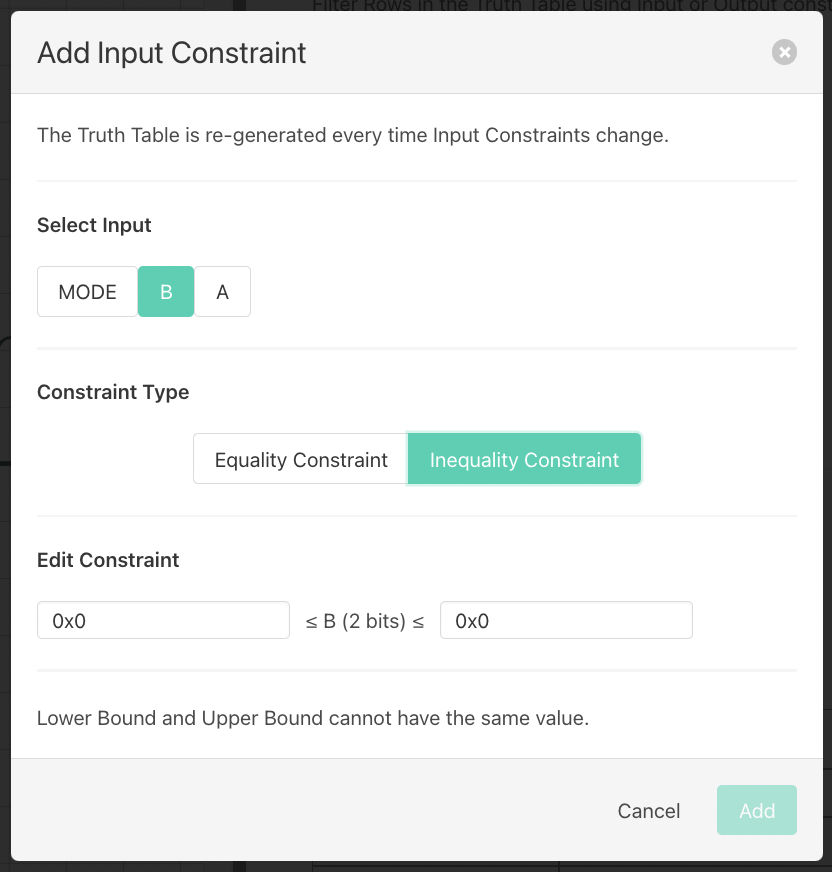
\includegraphics[width=\textwidth]{04.AnalysisDesign/constraintadder.png}
         \caption{Popup for Adding an Input Constraint}
         \label{fig:addconstraint}
     \end{subfigure}
     \begin{subfigure}[b]{0.4\textwidth}
         \centering
         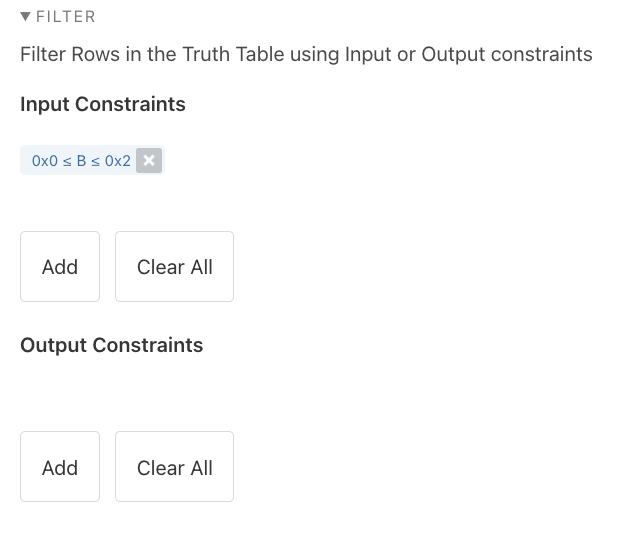
\includegraphics[width=\textwidth]{04.AnalysisDesign/tabwithconstraint.png}
         \caption{Filter section after adding a constraint}
         \label{fig:tabwithconstraint}
     \end{subfigure}
        \caption{Adding a Constraint to the Truth Table}
        \label{fig:constraintadd}
\end{figure}

\section{Hiding Output Columns}
The second menu section allows the user to hide (or un-hide) output or viewer columns from the truth table. This means that the user can choose to focus on relationship between the inputs and a specific output. This may be useful when analysing arithmetic circuits -- the user may wish to hide the carry-out column to only focus on the result. As can be seen in Figure \ref{fig:expand}, each output/viewer has a toggle component which has two options: visible and hidden. These are used to set the visibility of columns in the truth table. The action of hiding at output column takes less than 100ms -- this is classed as instantaneous. Achieving this required specific decisions to be made regarding how to the truth table was rendered; these will be discussed in Section \ref{sec:ttView}.

\section{Graphical Manipulation of Truth Tables}
\textbf{Re-ordering Columns} On either side of each IO label in the heading row, there are left and right arrows. These allow the user to arrange the truth table as they please by changing the order of columns in the truth table.

\textbf{Sorting} In each IO heading cell, there are a pair of up/down arrows for sorting the truth table by the values of that IO. Selecting the up arrow sorts in ascending order, while selecting the down arrow sorts in descending order. Once selected, an arrow remains highlighted (until another is selected), to inform the user of how the truth table is being sorted. The rationale behind implementing truth table sorting is that it allows users to organise the information they view, increasing the control they have over their learning experience. 

\textbf{Auto-resize with dividerbar} The draggable dividerbar can be used to resize the right section. The truth table will dynamically resize to match the set right section width, and contents of cells will wrap to the next line and automatically adjust such that no content is cut off.

All of the operations above happen instantaneously (<100ms); achieving such performance with column-based operations relied on the same decisions as those which made hiding columns appear instantaneous (see Section \ref{sec:ttView}).

\section{Don't Care Reduction} \label{sec:dcreductionanalysis}
If the generated numeric truth table is \textbf{not truncated}, then the user can reduce it through Don't Care reduction. When the user presses the \textit{Reduce} button, the truth table will be analysed, and any rows where certain inputs are redundant will be collapsed, with the value for that input being replaced by an \textbf{X}. The user can always return to the full table by clicking the \textit{Back to Full Table} button. Like their full numeric counterparts, reduced truth tables can also be filtered and sorted.
If the truth table is truncated, Don't Care reduction is unavailable; this is communicated to the user by a greyed-out \textit{Reduce} button. Hovering over the disabled button will show the user a popup explaining why the option is unavailable.

As discussed in Section \ref{subsec:dcbackground}, two possible methods of implementing DC Reduction were considered; either porting an existing heuristic-based minimisation tool to Issie, or writing a reduction algorithm from scratch. Ultimately, the latter was chosen. This is because existing minimisation tools are tailored towards hardware design in industry, where the priority is simplifying the design so it requires fewer components. There is a risk that complicated simplification may in fact obscure the logic further; this is the opposite of this project's intention. Further to this, current minimisation tools like Espresso \cite{espresso} do not support multi-bit inputs and outputs, which would make integration with Issie's existing framework difficult. Given the decision to not split up multi-bit IOs in Issie, Espresso was deemed unfit. The custom reduction algorithm takes an un-truncated numeric truth table and attempts to reduce it by recursively finding redundancies through row comparisons.

\section{Algebraic Truth Tables}
In addition to numeric truth tables, this project also adds algebraic truth tables to Issie. Instead of numerical values, outputs are instead represented as an algebraic function of their inputs. These algebraic functions are loosely based on Boolean algebra, but do include other operators such as addition and subtraction in order to provide a more useful summary of relationships. Users can introduce algebra into an existing numeric truth table by clicking the \textit{Algebra} button above the truth table. This will spawn a popup, where the user can choose which inputs to set as algebraic, and which inputs should remain numerical. There exist cases when certain inputs cannot be set as algebra, such as when an input is connected to the select (SEL) port of a multiplexer. The user is prevented from setting those inputs as algebraic values, and a helpful error message informs the user why. An example of this can be seen in Figure \ref{fig:algpopup}

\begin{figure}
    \centering
    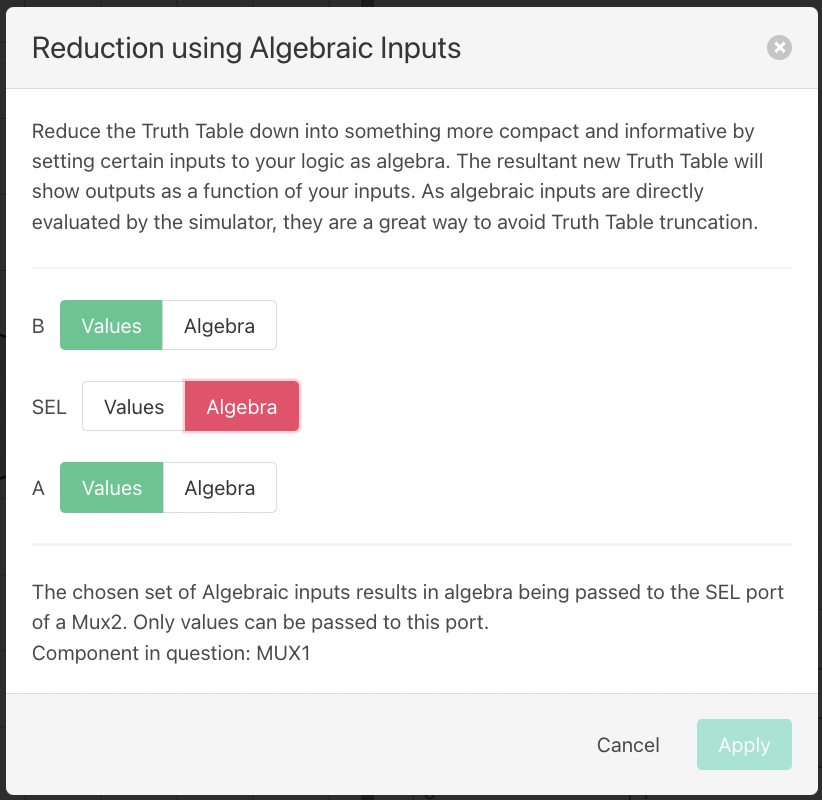
\includegraphics[width=0.6\textwidth]{04.AnalysisDesign/algebrapopup.png}
    \caption{Algebra Input Selector popup}
    \label{fig:algpopup}
\end{figure}

\subsection{Designing the System for Algebra}
The design of the system for the generation of Algebraic Truth Tables was one of the most complex activities undertaken by the project, with numerous decisions being taken regarding which features to implement and the overall approach to take. The requirements stated that support for circuits containing combinations of multiplexers and adders was the bare minimum (\textbf{D1.1.1}), but ideally Issie should support algebra for most combinational circuits.

\subsubsection{Decision 1: Algebraic Reduction vs Algebraic Generation}
It was originally envisaged that algebraic truth tables would be obtained through reduction. An exhaustive numeric truth table would be generated, and algebraic relationships would be inferred from it. This could possibly have been achieved through converting the truth table into SOP form, and then reducing the resultant Boolean equation using algebraic identities or existing logic minimisation tools like Espresso. However, following some analysis of this approach, it was deemed unfit. The requirement for an exhaustive truth table limits algebraic reduction to small circuits, while the nature of multi-bit inputs in Issie makes existing  minimisation techniques difficult to integrate into the application. Therefore, it was deemed that reducing a numeric truth table to create an algebraic truth table was not a viable strategy. his meant that algebraic truth tables would have to be generated directly from the schematic.

\subsubsection{Decision 2: Schematic Analysis vs Schematic Simulation}
Following the conclusion that algebraic truth tables would have to be directly generated from the schematic, two approaches for doing so were considered. The first was to analyse the schematic and attempt to match it to a specific case (e.g. a multiplexer circuit). The idea was that each case would describe a pre-defined algebraic relationship, which would then be returned to the user. It was thought that the approach could be extended to more complex circuits by recursively searching for cases contained within the circuit. 
The second approach was far more general; introduce a method for simulating a sheet in Issie with algebraic inputs and outputs. This would be implemented as an extension to the Fast Simulator.

The advantage of the first approach was that Requirement \textbf{D1.1.1} would be fulfilled quite easily. Following the experience of writing the Canvas Correction algorithm, it was known that checking for specific cases in the canvas state was possible, and therefore recognition of multiplexer and adder circuits could be implemented quickly. However, extending it further than that could be more challenging; the canvas state is closely related to how the user has built the schematic, and there are many different ways of implementing the same logical function. Therefore, adding support for complex relationships would likely require many cases to be checked. Furthermore, repeatedly checking the canvas state for increasingly complicated cases would increase the generation time. On the other hand, adding algebra to the Fast Simulator would be a lengthy process, increasing the amount of time required to complete \textbf{D1.1.1}. However, as the Fast Simulator is already compatible with all correct Issie schematics, it would be easier to extend algebraic simulation, as required by \textbf{D1.1.2}. Merely modifying the Fast Simulator would also introduce fewer lines of code into the Issie codebase, making further maintenance easier. Additionally, adding algebraic simulation to the Fast Simulator would mean that the Step Simulator, in theory, would also be able to support algebra. 

With all points considered, algebraic simulation was chosen over analysing the schematic. The Fast Simulator has been augmented so that it can receive both numeric and algebraic values as inputs to a simulation. It will then return outputs as functions of the algebraic inputs.


\section{Considering Logic Input with Truth Tables}
TBA


% \subsection{Generating Numeric Truth Tables}
% The primary aim of the project was the generation of truth tables with interactive features to aid in logic visualisation. Thus truth table generation lies at the is a key part of the application logic. When the user first generates a truth table by clicking on the \textit{Generate Truth Table} button, a numerical truth table is generated and shown to them.
% At its core, generating a complete numeric truth table is a brute-force process. Each possible combination of input values must be simulated to calculate the corresponding output values, and the relationship should be recorded in the table. 
% Given that Issie already features a performant and reliable simulator (step simulator) for calculating the outputs of combinational logic, the decision was made to use as much of its implementation as possible. This approach has many advantages:
% \begin{itemize}
%     \item The existing step simulator has been extensively tested by end-users, meaning that its implementation is most likely bug-free. By using it, it will reduce the chance of the new feature introducing new bugs.
%     \item In most cases, reusing existing code is much faster than writing new code from scratch. Not only is time saved on writing new code, but the amount of time spent debugging is also reduced.
%     \item Reusing existing code will help keep the overall size of the codebase small. Not only does this help future programmers who work on the project by reducing how much they have to understand, but it also means that any future improvements made to the simulation code are also improvements to Truth Table generation.
% \end{itemize}

% Figure \ref{fig:flowchartSim} provides an overview of Issie's process for building and running a Step Simulation. In this process, various checks must be performed; firstly the logic designed by the user must be verified to be syntactically correct, secondly the organisation of project files must be correct, and thirdly some Issie specific limitations (e.g. no cycles in combinational logic) must be enforced. Issie's simulation building process can be said to have three levels, with each level having an associated data structure which represents schematic. These data structures are: the \textbf{Canvas State}, \textbf{Simulation Data/Error}, and a \textbf{Fast Simulation}. A set of checks are performed at each level, and only upon passing these checks can a schematic be transformed to the subsequent data structure.
% If any of these checks fail due to an issue with the user's schematic, the simulation building process returns a \textit{SimulationError}, which tells the user what the error is and which components/connections are affected. A key takeaway from Figure \ref{fig:flowchartSim} is that the process of building a simulation is separate to the process of running it. During the \codestyle{FastSimulation} building process, the schematic is analysed, with components being placed into an appropriate order for combinational reduction. However, as the \codestyle{FastSimulation} data structure is mutable, the values of each input can be updated without having to rebuild the whole simulation. Therefore, the time taken simulating a different input combination is quite short, as only the reduction function has to be re-run to find the new outputs. 
% This distinction between building a simulation and running it with different input values makes the existing Step Simulator an optimal choice for use in truth table generation, which will need to simulate multiple input combinations as fast as possible. 

% \begin{figure}
%     \centering
%     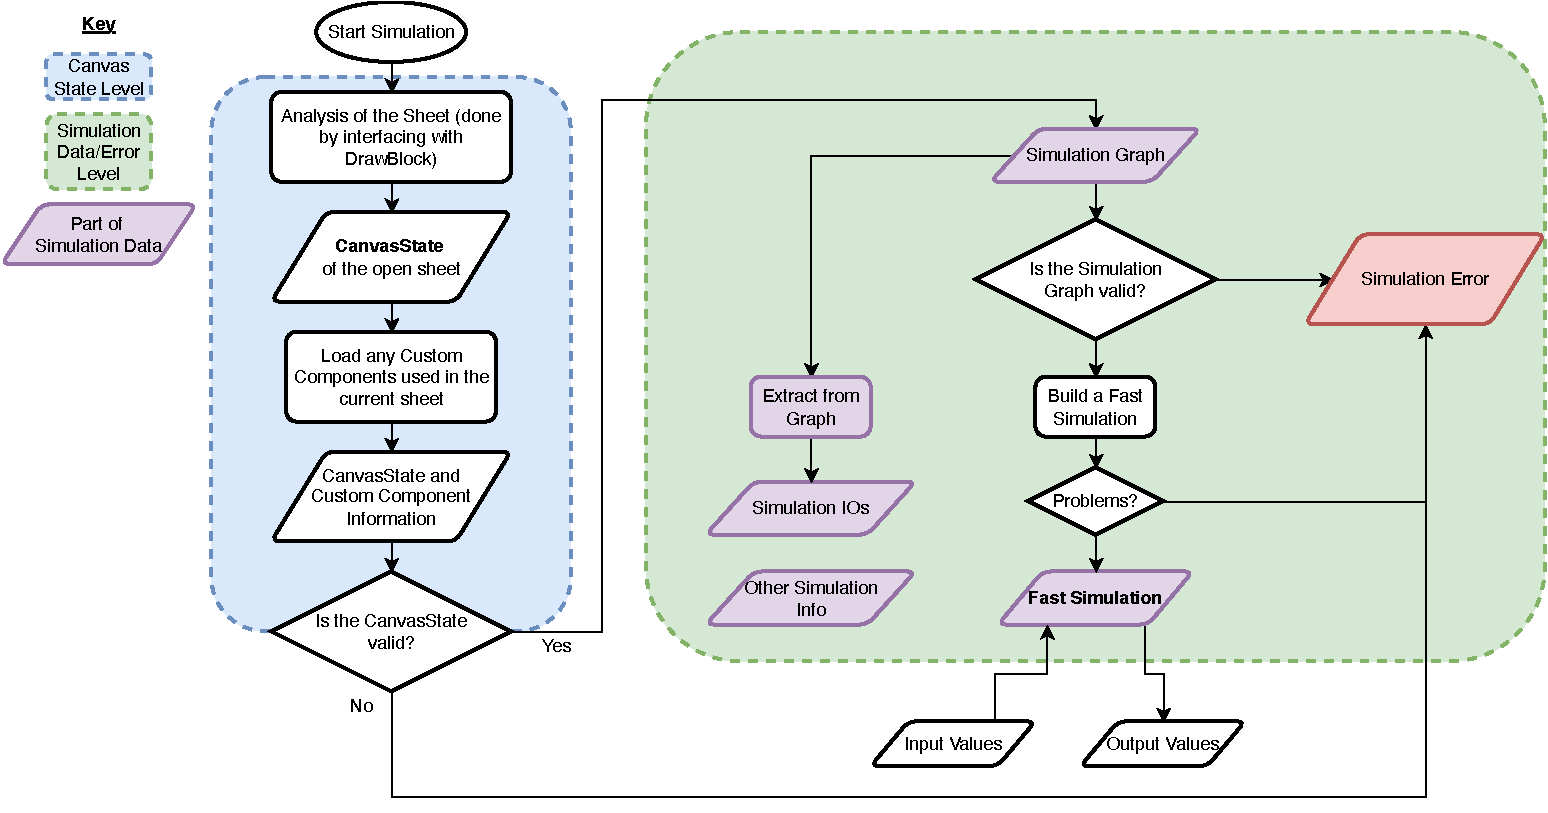
\includegraphics[width=\textwidth]{04.AnalysisDesign/IssieSim.pdf}
%     \caption{An overview of Issie's Step Simulation}
%     \label{fig:flowchartSim}
% \end{figure}

% Figure \ref{fig:ttGen} shows a high-level view of truth table generation in Issie. A simulation for the sheet is built using data stored in the current application state -- when generating truth tables for the whole sheet, this process is the same as the one which happens when starting the Step Simulator. When generating a truth table for a partial selection of a sheet, a few extra steps are required prior to the simulation building logic being called. The Step Simulator informs users of the correctness of their schematic through colour coded buttons. If the schematic is correct, the user will be shown a green button which allows them to start a simulation. On the other hand, if there are mistakes in the schematic, the user will instead be shown the \textit{See Problems} button, which will explain the nature of the Simulation Error. This functionality is replicated for the truth table, as it clearly informs the user of errors in their schematic. An additional check is also implemented for truth tables; the schematic must \textbf{only contain combinational logic}.

% If the checks for correctness and combinational logic pass, truth table generation can proceed. Alongside the Simulation Data, the truth table generation logic also requires information such as the input constraints and which inputs are algebraic. In Issie, truth tables are initially generated without any constraints or algebraic inputs, and are re-generated when these are added. Therefore, when the user clicks the button, these parameters are empty. From this information, the input space of the truth table (its left-hand side) is determined. Each input combination is then simulated, with the output and viewer values corresponding to that combination recorded and stored. A truth table is simply the mapping between input and output combinations - this mapping is stored so that it may later be viewed in tabular form by the View function.

% \begin{figure}[h]
%     \centering
%     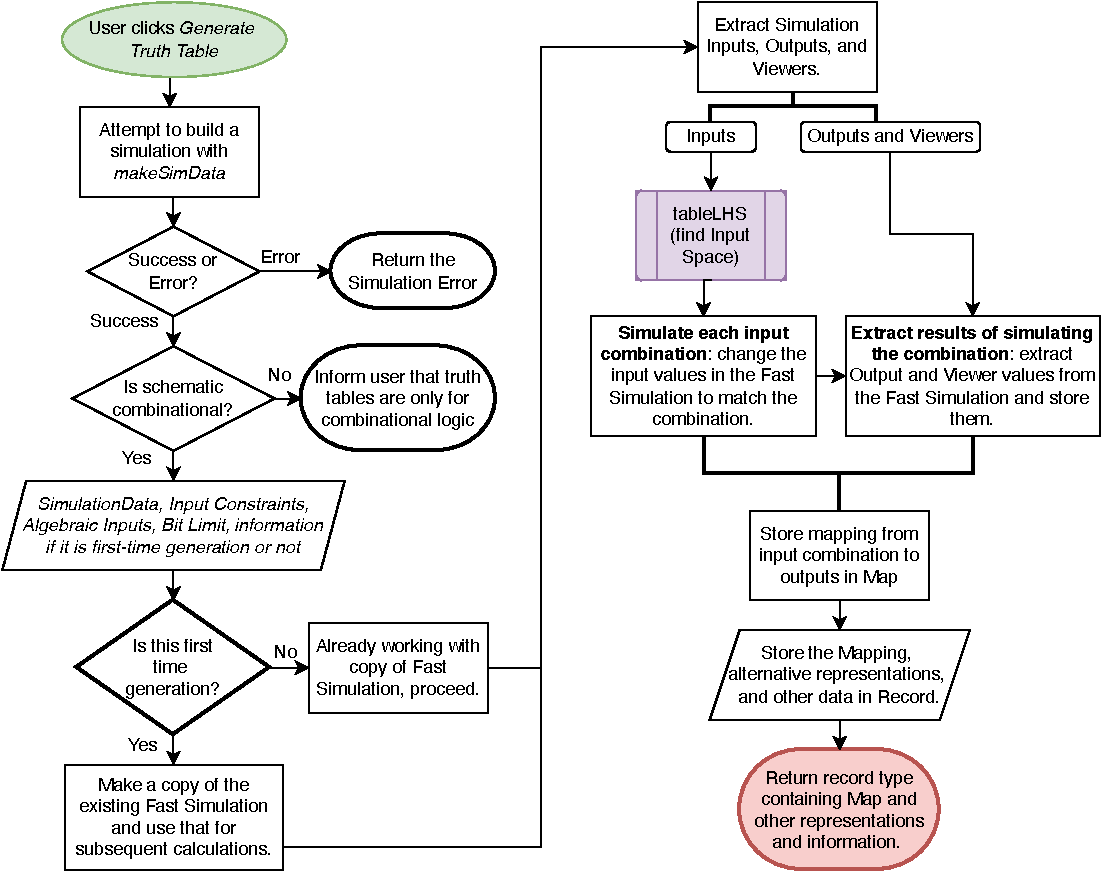
\includegraphics[width=\textwidth]{04.AnalysisDesign/ttGen.pdf}
%     \caption{High-Level view of Truth Table Generation}
%     \label{fig:ttGen}
% \end{figure}

% The process of calculating the input space, highlighted in purple in Figure \ref{fig:ttGen} had two versions; the change from the first to the second affected the overall structuring of operations on truth tables in the application. Initially, the entire input space was calculated and simulated. This would result in a very large, exhaustive truth table -- one which contained every possible input and output combination. The user would haven been able to reduce this truth table by filtering the table or using Don't Care Reduction. However, several issues arose with this approach, with the most crucial being that of performance. The complexity of finding the Cartesian product of multiple sets is an exponential function of the number of sets. For example, the complexity of finding the Cartesian product of $n$ sets, each of size $s$, would be $O(s^n)$. The size of each set is dependent on the width of the input; Issie does not limit input widths, meaning that the size of the sets may also be very large. For example, a single 16-bit input has 65536 unique values, and combining this with a second 16-bit input yields an input space of over 4 billion unique combinations. Simulating this large number of combinations and storing the result takes upwards of 20 seconds, violating essential requirement \textbf{E1.7}. Additionally, a sufficiently large input space could cause the system to run out of memory and crash, which is totally unacceptable. Along with the practical issues with the generation of the complete truth table, it can also be argued that a very large complete truth table is not useful to the user. According to the Atkinson-Shiffrin memory model described in Section \ref{subsec:memmodels}, external stimuli only stay in the sensory register for 0.5 seconds prior to decaying. A large number of rows is likely to overload the sensory register, meaning that it is likely that the information will not pass to short term memory unless the the user slows down and processes each row one-by-one. Even if this were the case, a truth table with a large number of rows would take over 30 seconds for the user to read and process. Given that short term memory decays in 30 seconds, this means that the user will likely have forgotten the first row by the time they finish reading the last one. Therefore, the method of generating and simulating the entire input space to create an exhaustive truth table was deemed unfit.

% As a result, the decision was made to \textbf{truncate the truth table}; generate and simulate only part of the input space. The current limit is 1024 rows. Considering that users would only be able to focus on a small subset of rows at a time, and would likely reduce the size of the table anyways, this approach would sacrifice very little for a significant gain. However, any subsequent operations, such as filtering and reduction, would take place on the truncated table, which does not contain all of the necessary data. The nature of these issues, as well as the steps taken to mitigate them are:

% \begin{itemize}
%     \item[] \textbf{Issue 1}: Input constraints will be applied to the truncated table, so user may not see a full representation of the relationships for the case they enter. For example, consider the input $X$ which has a width of 8 bits (so values range from 0 to 255), but due to truncation, only rows with values of $X$ up to 31 are present. If the user applies the input constraint $X = 32$ to the table, an empty table will be returned as no rows which fulfil this condition exist in the truncated table.
%     \item[] \textbf{Solution 1}: Apply input constraints during truth table generation. This is achieved by using the constraints to determine a tighter input space, and then simulating that. Giving users a way to choose which inputs contribute more to the input space (they can fix certain inputs and let others vary within bounds) allows them to interactively generate truth tables that deliver the most information to them.
%     \item [] \textbf{Issue 2}: Output constraints will be applied to the truncated table, which is missing many rows. Due to this, the result of applying the output constraints will include all rows which match the condition.
%     \item [] \textbf{Solution 2}: Unfortunately there is not much that can be done to combat this issue alone other than warn the user that they are looking at incomplete results. However, if the user is able to use input constraints to sufficiently reduce the input space first, output constraints could help filter the table further.
%     \item [] \textbf{Issue 3}: Don't Care Reduction will occur on the truncated table, which does not fully represent the logical function performed by the circuit. This could result in incorrect relationships being inferred by the reduction algorithm.
%     \item [] \textbf{Solution 3} Much like with output constraints, there is no perfect solution as relationships for reduction are inferred from the truth table. Don't Care reduction is therefore limited to smaller schematics which do not produce truncated truth tables. The user is instead guided towards reducing truth tables for larger schematics with \textbf{Algebraic Reduction}.
% \end{itemize}

% Implementing Solution 1 required a new method of generating the input space; a general view of the method used is shown in Figure \ref{fig:tableLHS}. As generating input combinations is expensive in terms of time and memory, the input space generation method needs to know which sub-sets of the input space it can and cannot generate before it actually generates it using the Cartesian product method. Further details of how this is implemented can be found in the Implementation chapter, with elaboration on the complex \codestyle{inputsWithARC} function (highlighted purple on Figure \ref{fig:tableLHS}).
% \begin{figure}
%     \centering
%     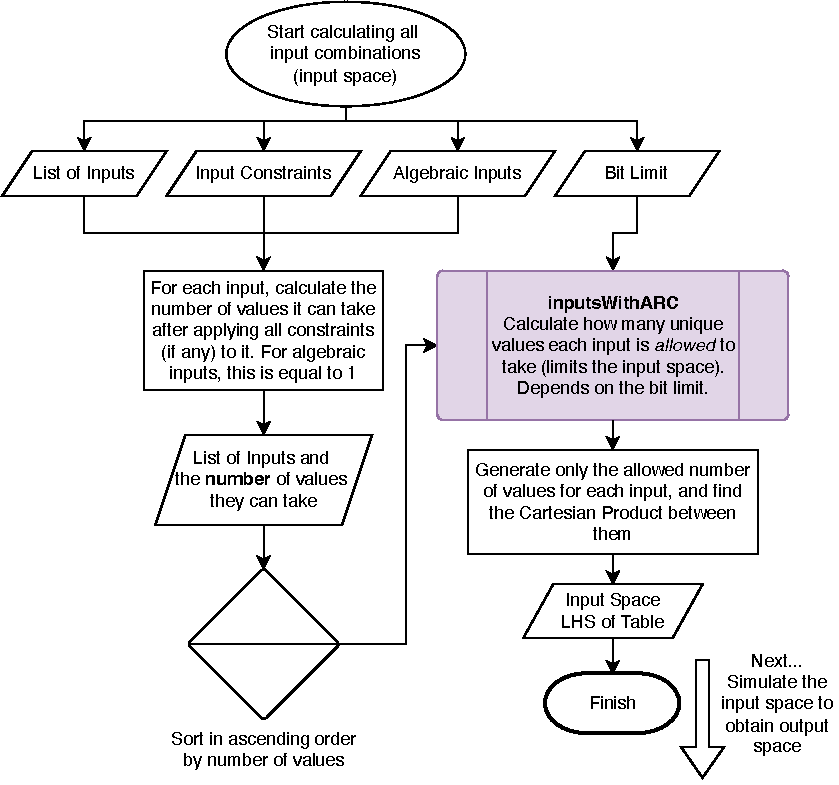
\includegraphics{04.AnalysisDesign/newLHS.pdf}
%     \caption{High-Level view of how the Input Space is generated}
%     \label{fig:tableLHS}
% \end{figure}
\chapter{Implementation}

\section{Overview of Data Types}
Various new F\fsharp types have been introduced to Issie by this project. This section describes these types and provides context to them, explaining their function and the rationale behind their creation.

\subsection{Types for Representing Truth Tables}
%%%%% Commands (variables) for type information %%%%%
% Cell Table Data
\newcommand{\ttCellData}{
    Discriminated Union type representing what data each truth table cell can hold. Cells can hold Bits (represented by Issie's WireData type), Algebraic expressions (represented by strings), or a Don't Care.
}

% Cell Table Data
\newcommand{\ttCellIO}{
    Discriminated Union type representing which input or output of the logic the data belongs to. \codestyle{CellIO}s can either be the existing \codestyle{SimulationIO} type used to describe Inputs and Outputs, or Viewers.
}

% TT Cell
\newcommand{\ttCell}{
    Record type which represents the contents of a cell in a truth table. Is made up of a \codestyle{CellIO} and some \codestyle{CellData}.
}

% TT Row
\newcommand{\ttRow}{
    Represents a row in a truth table, which is a list of Truth Table Cells.
}

% TT
\newcommand{\truthtable}{
    Record type containing various \codestyle{Map} data structures which map a row of inputs to a row of outputs. Different map data structures are used for caching different versions of the truth table. The record also contains fields and methods which contain or relay other metadata about the truth table.
}

\begin{table} [h!]
    \centering
    \begin{tabular}{| m{4cm} | m{10cm} |}
        \hline
        \textbf{Data Type/Structure} & \textbf{Information} \\
        \hline
        Cell Data & \ttCellData \\
        \hline
        Cell IO & \ttCellIO \\
        \hline
        Truth Table Cell & \ttCell \\
        \hline
        Truth Table Row & \ttRow \\
        \hline
        Truth Table & \truthtable \\
        \hline
    \end{tabular}
    
    \caption{Data Types and Structures used for Truth Table Representation}
    \label{tab:tabledatastructs}
\end{table} 

Truth tables in Issie are mostly stored as a mapping from input rows (each containing a single input combination) to output rows. This is implemented using the F\fsharp \codestyle{Map} type; therefore a truth table map has the type \codestyle{Map<TruthTableRow,TruthTableRow>}. The F\fsharp Map type implements immutable maps based on binary trees, which have a lookup time complexity of $O(log(n))$ \cite{fsmaps}. This is an improvement on traditional lists and arrays, which have a lookup time complexity of $O(n)$. Maps were chosen to store truth tables as it would be faster to look up an output row using a given input row.
The \codestyle{TruthTable} data type is a record containing fields which store cached truth table representations, as well as other data. The fields of this record are described in Table \ref{tab:ttRecord}. Caching different versions of the truth table trades a slightly increased memory usage for time saving, as operations on the truth table do not need to be re-applied every cycle of the view function.

\begin{table}[!ht]
    \centering
    \begin{tabular}{|m{6cm}|m{8cm}|}
    \hline
        \textbf{Field and Type} & \textbf{Explanation} \\ \hline
        \shortstack{TableMap: \\ \codestyle{Map<TruthTableRow,TruthTableRow>}} & The result of truth table generation. Contains the initially generated truth table with input constraints and algebraic inputs applied. \\ \hline
        \shortstack{DCMap: \\ \codestyle{Map<TruthTableRow,TruthTableRow>}} & The result of performing Don't Care Reduction on TableMap. Is an Option type, so is none if the table has not been DC Reduced. \\ \hline
        \shortstack{FilteredMap: \\ \codestyle{Map<TruthTableRow,TruthTableRow>}} & Cached result of filtering TableMap or DCMap with output constraints. \\ \hline
        SortedListRep: \codestyle{TruthTableRow list} & The result of sorting the truth table stored in FilteredMap. The truth table is stored as an ordered list because Maps in F\fsharp are unordered. \\ \hline
        IsTruncated: \codestyle{bool} & True if the truth table had to be truncated in the generation process. \\ \hline
        MaxRowsWithConstraints: \codestyle{int} & The number of rows the truth table should have after applying input constraints, but prior to truncation. Used to calculate how many rows have been lost to truncation. \\ \hline
        TableSimData: \codestyle{SimulationData} & Simulation used for the truth table, cached for use during table re-generation. \\ \hline
        IOOrder: \codestyle{CellIO list} & List of all CellIOs in the truth table, in the order they originally were when the truth table was generated. \\ \hline
        (member) Inputs: \codestyle{CellIO list} & Member function which returns a tist of all inputs in the truth table. \\ \hline
    \end{tabular}
    \caption{Explanation of \codestyle{TruthTable} Record fields}
    \label{tab:ttRecord}
\end{table}

\subsection{Constraint Types}
This project adds two types of numerical constraints; equality constraints and inequality constraints, the type definitions for which can be seen in Listings \ref{lst:equalitycon} and \ref{lst:inequalitycon}. Equality constraints on an input or output are of the form $IO = value$, where the truth table is filtered such that only rows where the input or output (IO) is equal to the given value are shown. Inequality constraints are of the form $LowerBound \leq IO \leq UpperBound$; the filtered truth table will only contain rows where the IO is between the lower and upper bounds (inclusive). There is also a \codestyle{ConstraintType} DU which differentiates between Equality (\codestyle{Equ}) and Inequality (\codestyle{Ineq}) constraints.

\begin{center}
\noindent\begin{minipage}{.45\textwidth}
\begin{lstlisting}[caption=Definition for Equality Constraint,frame=tlrb, language=FSharp, label=lst:equalitycon]{Name}
type EqualityConstraint = {
    IO: CellIO
    Value: int
}
\end{lstlisting}
\end{minipage}\hfill
\begin{minipage}{.45\textwidth}
\begin{lstlisting}[caption=Definition for Inequality Constraint,frame=tlrb, language=FSharp, label=lst:inequalitycon]{Name}
type InequalityConstraint = {
    LowerBound: int
    IO: CellIO
    UpperBound: int
    Range: int
}
\end{lstlisting} 
\end{minipage}
\end{center}

A set of constraints is therefore simply a list of all equality constraints combined with a list of all inequality constraints. This is the definition of the \codestyle{ConstraintSet} type.

\subsection{Algebra Types}
\subsubsection{Algebraic Operators} \label{subsubsec:imp_algebraops}
Table \ref{tab:algebraops} in Section \ref{subsec:algebraops} describes the algebraic operators the user may encounter in Issie. This sub-section describes the F\fsharp implementation of these operators. Algebraic operators in Issie are split into three Discriminated Union types: binary operators (\codestyle{type BinaryOp} which have two operands, unary operators (\codestyle{type UnaryOp}) which have one operand, and comparison operators (\codestyle{type ComparisonOp}). Currently, the there is only one comparison operator: \codestyle{Equals}, which compares an algebraic expression to an unsigned integer value. Listings \ref{lst:binaryop} and \ref{lst:unaryop} show all the different cases of binary and unary operators. There is one key omission from F\fsharp binary operators; the Append Operator. Initially, this was implemented as a binary operator, joining the two operands. However, in circuits with multiple connected \textit{MergeWires} components, a chain of nested append operators would form. Figure \ref{fig:mergewires} shows such a circuit. Expression \ref{equ:longappend} is the result of performing algebraic simulation when appends were implemented as binary operators. It features three pairs of parentheses which clutter the expression. In contrast, Expression \ref{equ:shortappend} communicates the same information without brackets. This cleaner expression was obtained by representing append operations as lists of expressions during algebraic simulation. This list itself is treated as an algebraic expression -- the nature of algebraic expressions in Issie is explained in Section \ref{subsubsec:imp_algebraexps}. A list representation is also easier to analyse, meaning that specific patterns in appends can be inferred. For example, successive appends of consecutive bits of the same IO ($A[7]::A[6:3]::A[2]$) can be folded into one Bit Range operation ($A[7:2]$). 
\begin{center}
\noindent\begin{minipage}{.45\textwidth}
\begin{lstlisting}[caption=Definition for Binary Operators,frame=tlrb, language=FSharp, label=lst:binaryop]{Name}
type BinaryOp = 
    | AddOp // A + B (mathematical addition)
    | SubOp // A - B (mathematical subtraction)
    | BitAndOp // A & B (bitwise AND)
    | BitOrOp // A | B (bitwise OR)
    | BitXorOp // A XOR B (bitwise XOR)

\end{lstlisting}
\end{minipage}\hfill
\begin{minipage}{.45\textwidth}
\begin{lstlisting}[caption=Definition for Unary Operators,frame=tlrb, language=FSharp, label=lst:unaryop]{Name}
type UnaryOp = 
    | NegOp // -A (mathematical negation, bitwise two's complement)
    | NotOp // bit inversion (bitwise XOR with -1)
    | BitRangeOp of Lower:int * Upper:int // A[upper:lower] (subset of bits of A)
    | CarryOfOp
\end{lstlisting} 
\end{minipage}
\end{center}

\begin{center}
\noindent\begin{minipage}{.45\textwidth}
\vspace{-2ex}
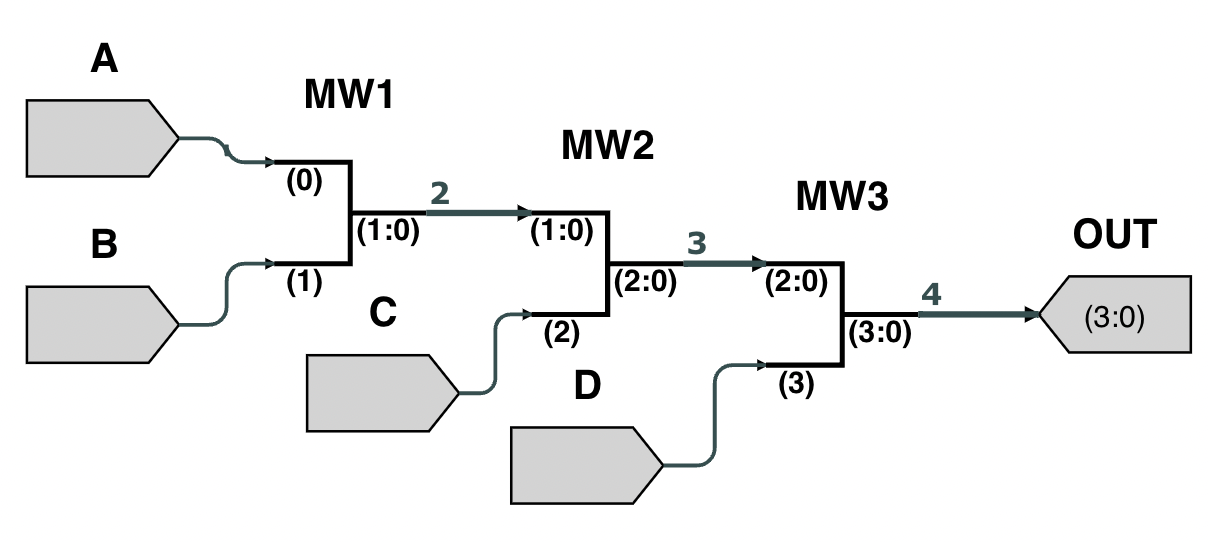
\includegraphics[width=1.0\linewidth]{05.ImpPlan/mergewires.png}
\captionof{figure}{\label{fig:mergewires}Circuit with multiple \textit{MergeWires} connected to each other}
\end{minipage}\hfill %
\begin{minipage}{.45\textwidth}
\begin{equation} \label{equ:longappend}
    OUT = (D::(C::(B::A)))
\end{equation}
\begin{center}
Append as a Binary Operator
\end{center}
\vspace{2em}
\begin{equation} \label{equ:shortappend}
    OUT = D::C::B::A
\end{equation}
\begin{center}
Append as a list of appended expressions
\end{center}
\end{minipage}
\end{center}

\subsubsection{Algebraic Expressions} \label{subsubsec:imp_algebraexps}
Using a DU type, a short grammar was written to represent algebraic expressions in Issie. The grammar writing process in particular validated the choice of F\fsharp as a programming language for the project; the DU type allows for the grammar to be defined succinctly (only 7 lines of code), while pattern matching on DUs enables evaluation of an expression through a single recursive function. Large class hierarchies are therefore not required. Algebraic expressions in Issie are defined by the type \codestyle{FastAlgExp} -- the prefix \textit{Fast} is used as the algebraic expressions are used within the Fast Simulation.

According to the grammar, an algebraic expression (\codestyle{FastAlgExp}) in Issie can be:
\begin{enumerate}
    \item \textbf{\codestyle{SingleTerm of SimulationIO}}: Represents a single algebraic term, which is an input. This case has the type \codestyle{SimulationIO} as every input in Issie is represented by that data structure.
    \item \textbf{\codestyle{DataLiteral of FastData}}: Represents a numeric value in the simulation. 
    \item \textbf{\codestyle{UnaryExp of Op: UnaryOp * Exp: FastAlgExp}}: Represents a unary expression. The unary operator (\codestyle{Op}) takes the expression (\codestyle{Exp}) as its operand. An example would be $-A$.
    \item \textbf{\codestyle{BinaryExp of Exp1: FastAlgExp * Op: BinaryOp * Exp2: FastAlgExp}}: Represents a binary expression, in which a binary operator (\codestyle{Op}), such as '$+$', operates on two expressions. \codestyle{Exp1} is the left operand, \codestyle{Exp2} is the right operand.
    \item \textbf{\codestyle{ComparisonExp of Exp: FastAlgExp * Op: ComparisonOp * uint32}}: Represents a comparison between an algebraic expression (\codestyle{Exp}) and a numeric value.
    \item \textbf{\codestyle{AppendExp of FastAlgExp list}}: Represents an expression that is made up of a group of existing expressions appended together. The list is ordered such that the most significant bit is at the head of the list. F\fsharp lists are are implemented as singly-linked-lists, therefore adding a new item to the head of a list is an $O(1)$ operation. Therefore, having the MSB at the head of the list means that appending something further onto the \codestyle{AppendExp} is efficient.
\end{enumerate}

\subsection{The \codestyle{TableInput} Data Type}
The \codestyle{TableInput} data type is used when generating the input space of the truth table. As discussed in Section \ref{subsec:evolutionofinputspace}, the method for generating a limited input space needs to know exactly which specific input combinations to generate out of potentially billions of possible combinations. To achieve this, a new data structure for representing inputs was required; one which stores more than  the \codestyle{SimulationIO} type. The \codestyle{TableInput} is a record type, and its fields are described by Table \ref{tab:tableinput}.
The term \textit{Row Count} in the context of the input space generation refers to the size of the set ($S_i$) of unique values an input ($x_i$) can contribute to a table.

\begin{table}[!ht]
    \centering
    \begin{tabular}{|m{4cm}|m{9cm}|}
    \hline
        \textbf{Field and Type} & \textbf{Explanation} \\ \hline
        IO: \codestyle{SimulationIO} & Inputs in Issie are represented by the SimulationIO type, which contains the Component ID, Component Label, and the width of the input. \\ \hline
        IsAlgebra: \codestyle{bool} & True if the input is algebraic, as opposed to numeric \\ \hline
        MaxRowCount: \codestyle{int} & The total size of the Set $S_i$, which is equal to $2^{w_i}$, where $w_i$ is the width of the input. \\ \hline
        ConstrainedRowCount: \codestyle{int} & The size of the subset of $S_i$ which contains all input values which conform with the input constraints. For example, if there were the following constraints on the input: $0 \leq x \leq 6$ \& $x = 9$, the Constrained Row Count would be 8. Constrained Row Count is always less than or equal to Max Row Count. \\ \hline
        AllowedRowCount: \codestyle{int} & The number of input values the given input is actually allowed to contribute to the truth table. Ideally, this is equal to the Constrained Row Count, but in situations where the truth table has to be truncated, the Allowed Row Count may be limited to keep the total number of rows in the truth table under the overall limit. \\ \hline
    \end{tabular}
    \caption{Explanation of Fields in the \codestyle{TableInput} data structure}
    \label{tab:tableinput}
\end{table}

\subsection{Table Manipulation Data Types}
The following data types are used in messages sent from the view function to the update function to indicate that some UI interaction has occurred which requires updating certain parts of the model.

\subsubsection{When the Truth Table is out of date}
There are numerous operations a user can perform on a truth table. These range from adding input or output constraints to changing the order of columns. The actions render the displayed truth table out of date. Updating the truth table depends on the action performed as re-generating the table from scratch for all actions would be wasteful and inefficient. Therefore, the update function needs to know exactly which action caused the table to go out of date. This is the purpose of the \codestyle{ReasonOutOfDate} DU type. There are four reasons a truth table may be out of date:
\begin{itemize}
    \item \codestyle{Regenerate}: The truth table needs to be re-generated from scratch. This is due to a change in input constraints or algebraic inputs.
    \item \codestyle{Refilter}: Output constraints have changed, so the truth table needs to be filtered again using the updated constraints.
    \item \codestyle{ReSort}: The IO the table is to be sorted by and/or the order it needs to be sorted in has changed. Sort the table again to reflect this.
    \item \codestyle{HideCol}: An output column has been hidden or unhidden -- change the truth table to reflect this.
\end{itemize}
The circumstances in which these messages are sent, and what exactly happens when they are received will be covered in further detail later in this chapter.

\subsubsection{Truth Table Sorting direction}
\begin{lstlisting}[caption=Definition for Sort Type,frame=tlrb, language=FSharp, label=lst:ttsort]{Name}
type SortType = | Ascending | Descending
\end{lstlisting} 
As shown in Listing \ref{lst:ttsort}, sorting can be done in ascending or descending order.

\subsubsection{Changing the Order of Columns}
\begin{lstlisting}[caption=Definition for Movement Direction,frame=tlrb, language=FSharp, label=lst:ttmovecol]{Name}
type MoveDirection = | MLeft | MRight
\end{lstlisting} 
As shown in Listing \ref{lst:ttmovecol}, columns can be moved left or right.

\section{Top Level UI Changes}
\subsection{Simulation Sub-tabs}
All activities that involved some form of circuit simulation were organised under the \textbf{Simulations} tab (formerly called Simulation) using sub-tabs. The right section tabs are implemented with the Fulma \cite{fulmaio} Tabs component. The Sub-tabs are implemented by nesting a second Fulma Tabs component within the body of the Simulations tab, and making ensuring that a sub-tab is visible only when it and the parent tab is open.

\subsection{Moving the Waveform Simulator}
Due to its inconsistent placement and strange tab-spawning behaviour, the decision was made to move the waveform simulator into its own, permanent sub-tab. The move was quite straightforward; the \textit{Waveforms} button was moved to the sub-tab, a greeting was also displayed. However, one small change had to be made to how the waveform simulator operated. When a waveform simulation is running, other tabs in the app are inaccessible by design. Previously, the waveform simulation tab would only open when the user was either starting or viewing a waveform simulation. Therefore, the existence of the tab was a valid metric for ascertaining whether the app should make other functions inaccessible. Following the changes, however, the existence of the waveform simulation tab is independent of whether a waveform simulation is running. Therefore, a new pair of messages \codestyle{LockTabsToWaveSim} and \codestyle{UnlockTabsFromWaveSim} can be used to control when the user is locked into the Waveform Simulator.

\subsection{Dynamic Dividerbar Resizing}
The dividerbar is situated between the canvas and the right section and marks the boundary between the two. During waveform simulation, the dividerbar becomes draggable to let the user view more content by resizing the right section. This functionality was also extended to truth tables. However, there was a bug in the implementation of the dividerbar. The CSS Style for the dividerbar element sets its height to 100\% of the right section. If the height of the the content in the right section exceeds the initial height of the right section, the latter \textit{overflows} and becomes scrollable. The 100\% height styling on the dividerbar did not take the overflow into account, meaning that the dividerbar would slowly disappear off screen as the user scrolled down. This issue was fixed by getting the right section \codestyle{div} element from the DOM Tree, and reading its \codestyle{scrollHeight}, which takes overflow into account. 

\section{Generating Truth Tables}
Figure \ref{fig:ttGen} in Section \ref{sec:analysis_ttGen} described the high-level method for generating truth tables in Issie. In the interest of consistency for both the user and future developers, as well as ease of maintenance, the truth table generation code either uses the Step Simulator code, or conforms with its design language.



% For only two multi-bit inputs, the library function \codestyle{List.allPairs} \cite{ListFuns} can be used to find this Cartesian product, with each set of possible values being passed in as a List. However, no such library function exists for $n$ sets/lists. The function \codestyle{numbComb} was implemented to find the Cartesian product of $n$ lists. The function is tail recursive for improved performance.




\subsection{Truth Table Generation Algorithm}
\emph{Associated Requirements:} \textbf{E1.1}, \textbf{E1.3}, \textbf{E1.6}


Figure \ref{fig:ttGen} shows a high-level view of the method used to generate truth tables in Issie. The user initiates truth table creation by clicking on a button. Following this, 

As outlined in the previous section, the major hurdle to overcome during truth table generation was the immense size of the input space, as generating and mapping a large input space to its corresponding output space was deemed both inefficient and unnecessary. The final generation algorithm solves this issue by limiting the maximum size the input space can grow to. If the truth table has more input combinations than the limit allows, the truth table is \textbf{truncated}, and only the maximum number of allowed rows are shown. Following some trial-and-error testing, a maximum value of 1024 ($2^10$) rows was chosen. This would allow for small circuits to be wholly represented by the generated truth table, while still allowing for relatively fast truncated truth table generation for larger circuits. The issue with using truncation alone is that the generated truth table does not fully represent the logic. Therefore, users may not be able to find specific rows in the truth table, and conclusions drawn from the truth table may not always be accurate. As a result, the final generation algorithm reduces the input space by \textbf{first applying input constraints, and then truncating if necessary}. If a user generated truth table is truncated, they are warned and it is suggested that they apply more restrictive input constraints to view a specific subset of the truth table.



\subsubsection{Algorithm for generating the Input Space}


\subsection{Numerical Constraints}
\emph{Associated Requirements:} \textbf{E1.5}

As per the requirements, users should have a way of filtering the truth table by applying numerical constraints to table inputs and outputs. This is necessary to reduce the size of the table and allow users to analyse relationships between inputs and outputs for a subset of the input space. 


% \subsubsection{Visualising Truth Tables}
% As of the Interim report, Truth Tables are visualised using Fulma Tables. They are clear, responsive and do a good job overall. However, they lack interactivity. Therefore, it is anticipated that they will be replaced or modified in the future. For viewing multi-bit inputs and outputs, hexadecimal was chosen over binary as it would take up less physical space. Currently, there is no option to change number base (as there is in the Step Simulator), but this would be trivial to implement in the future. Truth Table generation and viewing is done in an MVU way; pressing the "Generate Truth Table" button causes a truth table to be generated and stored in the \textbf{Model} through a message which is processed by the \textbf{Update} function. On the next call of the View function, this Truth Table is rendered.


\subsection{Generating Truth Tables for a partial selection of a Sheet}
\emph{Associated Requirements:} \textbf{E1.2}, \textbf{E1.3}

% The motivation behind Requirement \textbf{E1.2} is that a large schematic with lots of components will often contain smaller blocks of logic within it. These blocks may be defined Custom Components, or simply be a collection of gates in one corner of the canvas. Either way, there is value in the user being able to isolate these blocks and learn about the combinational logic implemented by them. Such functionality would also allow users to take a divide-and-conquer approach to debugging logical errors - individual blocks could be inspected to ascertain if they had been implemented correctly. 

% A challenge with generating a truth table from part of a canvas is that Issie has no existing method for simulating part of a canvas. When working with a whole sheet, the inputs and outputs are well-defined; sheets where any ports aren't connected to inputs/outputs throw \textit{Simulation Errors}. In contrast, a partial selection from a sheet will rarely contain all inputs and outputs. Two methods were considered for simulating the selected logic to generate a truth table, with the latter being chosen.
% \begin{enumerate}
%     \item \textbf{Extracting the Fast Simulation and feeding values into specific wires}. This method would have involved creating a Fast Simulation for the whole sheet as usual, but then manually changing values in component arrays and seeing how those changes propagated through to the output connections of the selected logic. While this method seemed fit initially, several issues were found after some analysis. The Fast Simulation would be built for the whole sheet, meaning that an error elsewhere on the canvas would stop the selected logic from being simulated. Custom Components would also be harder to manage as the Fast Simulation datatype flattens the design, meaning that all nested logic in Custom Components would be expanded out. The new logic would also be quite different from the truth table generation logic for whole sheets - this is not ideal for future code maintenance purposes.
%     \item \textbf{Intelligently building and correcting a new Canvas}. Following the highlighting of the issues with the first approach, an alternative approach was put forward. Rather than attempting to work with the complicated Fast Simulation data structure, it instead aims to use as much of the existing code as possible by treating the selected logic as a separate instance of a Canvas State and trying to simulate it using the same method as simulating a whole canvas. The main difference between simulating a whole sheet and simulating selected logic is the lack of guaranteed input and output components. This is overcome by finding which ports/connections are inputs/outputs for the selected logic, then intelligently adding 'phantom' input/output components to the canvas in a process called Canvas Correction. Once a corrected canvas corresponding to the selected logic is created, the logic used for generating and viewing a Truth Table for a whole sheet can be reused.
% \end{enumerate}

% Prior to the canvas correction stage, the selected components are checked. If only connections are selected, then a \textit{Simulation Error} is returned to the user informing them of their mistake.

\subsubsection{Canvas Correction}
\begin{itemize}
    \item[Step 1] \textbf{Add Extra Connections:} Sub-figures \ref{subfig:SelCase2} to \ref{subfig:SelCase4} in Figure \ref{fig:SelCases} all show situations where one or more inputs/outputs for the selected logic are ports on components, rather than connections. Taking the case shown in Figure \ref{subfig:SelCase2} in particular, the inputs to the selected logic are: both input ports on G1, and the bottom input port on G2, while the outputs from the selected logic are both output ports on G1 and G2 respectively. Prior to correction, the selection canvas does not have any connections going into those ports. This step finds any ports on selected components which do not have a connection in the selection and connects them to "dummy" input or output ports depending on their \codestyle{PortType}. This transforms the canvas to a state similar to that seen in Case (a), where   all inputs into the selected logic have connections.
    \item[Step 2] \textbf{Add Extra IOs:} This step adds the "phantom" input and output components to the selection canvas. The locations where these components need to be inserted are found by checking which connections in the Canvas State do not have both ports present in the selection. Any such connections are either connected to some other component in the sheet which is not selected, or are newly added connections which are connected to dummy ports. Either way, these are the connections that need to be connected to "phantom" IOs. 
    \begin{itemize}
        \item[Step 2.1] \textbf{IO Width Inference:} When creating new input or output components, the correct width must be specified. This is         calculated by running Issie's \codestyle{WidthInferrer} on the whole sheet to find the expected width of the input or output. However, in cases such as the one shown in Figure \ref{subfig:SelCase4}, where there are no connections to/from some ports on G3, \codestyle{WidthInferrer} will fail to infer widths, resulting in a \textit{Simulation Error}. A possible workaround would be to try to infer the width from the component itself if \codestyle{WidthInferrer} fails - in Issie AND gates always have 1-bit inputs, so any "phantom" inputs generated would have a width of one. This would be trivial to implement in the future. However, there would still be cases, such as inputs into multiplexers and n-bit XORs, where even this approach would not work.
        \item[Step 2.2] \textbf{IO Label Inference:} Usually users provide labels for IOs, which are used in the Truth Table. However, when IOs are automatically created, names for them must be automatically generated too. This is done by looking at which ports in the selection they are connected to. The expression for an automatically generated IO Label is: \codestyle{[Connected Component Label]\_[IN/OUT][SUFFIX]}. If the port is labelled (e.g. on a multiplexer or a Custom Component), the suffix is the port label. Alternatively it is the \codestyle{PortNumber}, which indicates the position of a port on its host component.
        
    \end{itemize} 
    \item[Step 3] \textbf{Returning a Canvas or an Error:} If any errors were found in the previous steps, most likely due to a malformed selection, they are returned. If not, then the returned Canvas State is completely compatible with the existing simulation and truth table generation functions.
\end{itemize}

Following Canvas Correction, any returned Canvas State is fully compatible with the existing functions for simulating logic and generating truth tables. Therefore, a Truth Table can be generated for selected logic through the same methods and functions used for generating Truth Tables for the whole sheet.

\bigskip
\begin{figure} [h]
    \begin{subfigure}{0.48\textwidth}
        \centering
        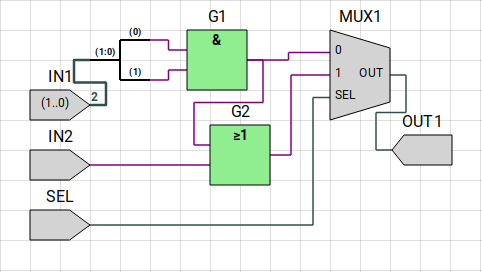
\includegraphics[width=0.8\linewidth]{05.ImpPlan/SelCase1.png}
        \caption{Case where all inputs into selected logic are connections.}
        \label{subfig:SelCase1}
    \end{subfigure}
    \begin{subfigure}{0.48\textwidth}
        \centering
        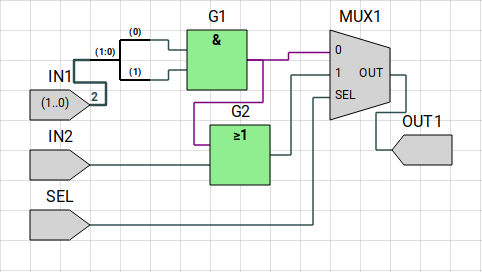
\includegraphics[width=0.8\linewidth]{05.ImpPlan/SelCase2.png}
        \caption{Case where some inputs into selected logic are connections, and some are ports on components.}
        \label{subfig:SelCase2}
    \end{subfigure}
    \newline
    \begin{subfigure}{0.48\textwidth}
        \centering
        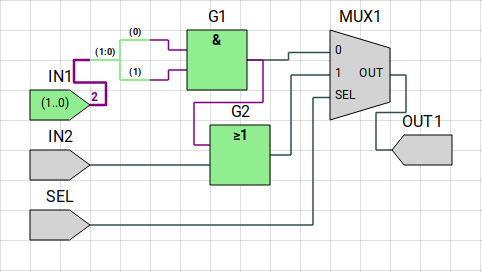
\includegraphics[width=0.8\linewidth]{05.ImpPlan/SelCase3.png}
        \caption{Case where selected logic includes an input component.}
        \label{subfig:SelCase3}
    \end{subfigure}
    \begin{subfigure}{0.48\textwidth}
        \centering
        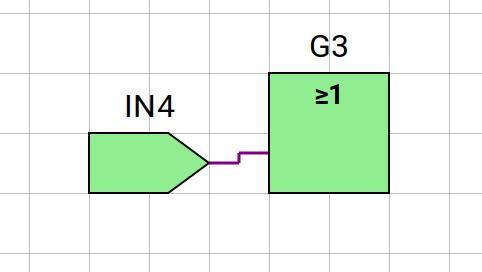
\includegraphics[width=0.8\linewidth]{05.ImpPlan/SelCase4.png}
        \caption{Case where a selected component does not have connections to all ports}
        \label{subfig:SelCase4}
    \end{subfigure}
    \caption{Selection Cases}
    \label{fig:SelCases}
\end{figure}

\subsection{UI Changes}
\emph{Associated Requirements:} \textbf{D3.1}
As mentioned in Section \ref{sec:IssieUI}, there are inconsistencies in Issie's current UI, particularly concerning the Waveform Simulator. With the addition of Truth Table viewing to Issie, the decision was made to tweak the UI to try to keep everything consistent. Figures \ref{fig:OldUI} and \ref{fig:NewUI} show the old and newly tweaked UIs respectively. The top bar primarily houses operations or information concerning files, such as the button to save the sheet, menu to open other sheets/projects, and the filepath. As a result the \textit{Waveforms} button has been removed from there. Ideally it would have a permanent place on the right tab, however with the addition of a Truth Table tab this would take the total number of tabs up to five, causing the tab label text to become illegible.  Given that there are now three ways to gain an insight into the logic on the sheet (Step Simulator, Truth Tables, Waveform Simulator), it is logical to group these together as sub-tabs under one main tab. The new UI now always has three tabs on the right in contrast to the old UI which would spawn the WaveSim tab when viewing Waveforms. Clicking the right-most "Simulations" tab will now reveal three sub-tabs: Step Simulation, Truth Tables, and Wave Simulation. The behaviour of the Truth Table view and the updated WaveSim view is modelled on that of the Step Simulator. Selecting a tab for the respective simulator will reveal a short description of the function, and a button to start the appropriate action. The colour and message shown by this button is dependent on the sheet: problems will show a yellow button, and a solid green button shows that the sheet is correct, and the functionality is available. Light green means that while the sheet is syntactically correct, some other factor is making the functionality unavailable. For the Waveform simulator this is when the sheet contains no synchronous logic (meaning no waveforms to display), and for Truth Tables it is when the sheet does contain synchronous logic (as synchronous logic is currently not supported for truth tables).

\begin{figure}
    \centering
    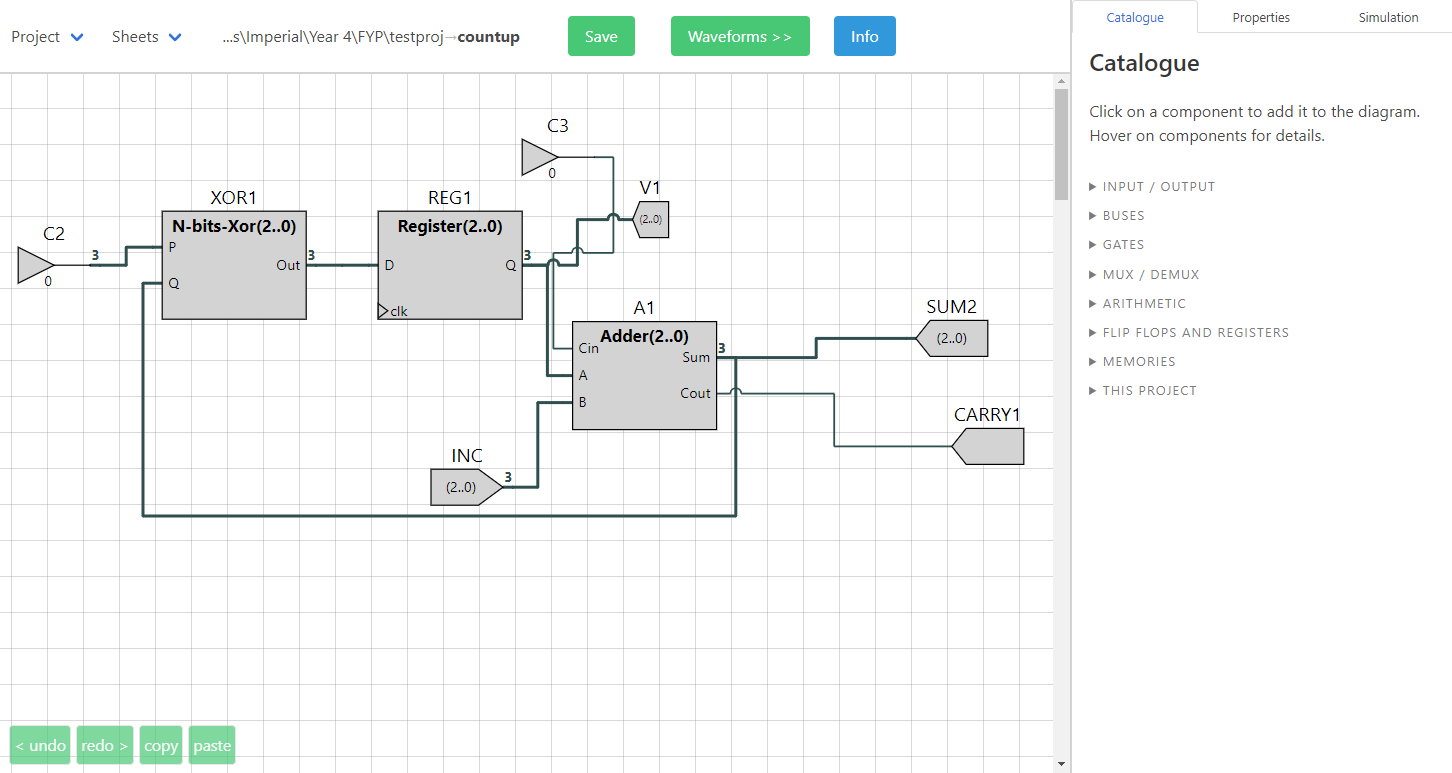
\includegraphics[width=0.8\textwidth]{05.ImpPlan/OldUI.png}
    \caption{Old Issie UI}
    \label{fig:OldUI}
\end{figure}

\begin{figure}
    \centering
    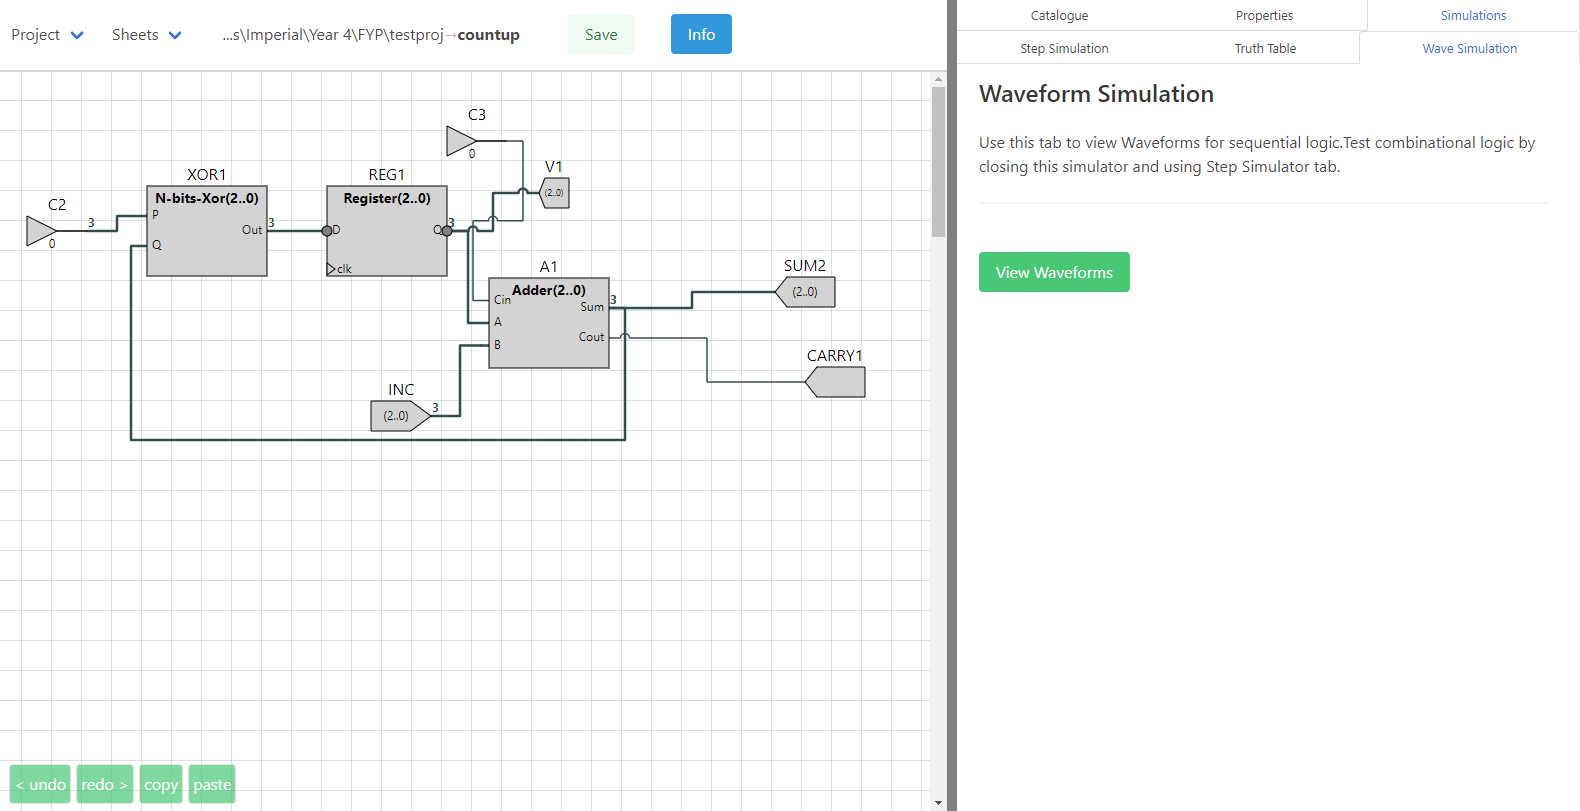
\includegraphics[width=0.8\textwidth]{05.ImpPlan/NewUI.png}
    \caption{New Issie UI}
    \label{fig:NewUI}
\end{figure}

\section{Work Breakdown Structure}
As with any large project, a key stage in planning is to break it down into several manageable chunks. This has been done to some extent in the Requirements Capture (Chapter \ref{chap:requirements}), albeit at quite a high level. On the other hand, a Work Breakdown Structure (WBS) \cite{projectmanagement} defines the scope of the project and breaks the work down into components that can be scheduled, monitored, and controlled. This aids in assessing the complexity of certain tasks, therefore improving the overall distribution of resources (mainly time) to different tasks. The WBS for this project is shown in Figure \ref{fig:wbs} - it is rotated to make it more clear to the viewer. Red nodes in the WBS could be considered as \emph{Initiatives}, as they are long term (relative to the length of the project) objectives. Green nodes are rough equivalents to \emph{Epics}, and white/grey nodes are \emph{User Stories}. In some cases, user stories may have very short sub-tasks underneath them which need not necessarily be differentiated, but are done on the WBS for clarity's sake. User Stories which spawn sub-tasks are coloured purple, while sub-tasks requiring further elaboration are coloured yellow. 

\section{Time Management and Gantt Chart}
Effective time management is vital to any project; traditionally a Gantt chart is used to display the timeframe in which the tasks detailed in the WBS will be completed. In line with this, a Gantt chart has been prepared for this project, and can be seen in Figure \ref{fig:gantt}. The colour coding on the chart matches that on the WBS, and key deadlines are indicated by dashed vertical lines. The first line represents the Interim report deadline - therefore any work shown on the chart to the left of this line is already completed, while any work to the right of the line is planned. The layout of Figure \ref{fig:gantt} allows it to double as a chronologically structured backlog. Within Initiatives, Epics are placed in chronological order, and likewise for User Stories within Epics. Two main considerations were made when devising this order of items. Firstly, dependencies were considered - for example it would be foolish to write code to view truth tables prior to there being a mechanism to generate them. Secondly, the importance of the deliverable associated with a task was taken into account - with tasks that fulfilled essential requirements given precedence over those that fulfilled desired requirements. 

\subsection{Contingencies and Strategies taken to Mitigate Risk}
The project plan has been structured to contain a healthy contingency allowance. Looking at the order of work in the Gantt chart, it can be seen that all essential requirements (and the majority of the desired features) should be fulfilled by the beginning of May. Furthermore, all technical work is expected to be completed by the end of May, bar a possible need to reconfigure parts of Issie's overall GUI (which is very unlikely).
Additionally, most time estimations for tasks have some margin built in as well, reducing the likelihood of technical work overrunning. This leaves the last three weeks of the project dedicated solely to report writing and documentation; two tasks which ideally will have been worked on over the duration of the project. Therefore, this plan yields a contingency allowance of three weeks.
The project management strategy, formed by a fusion of plan-based and Agile management methods, also acts as a form of contingency. As stated, the backlog ordering methodology has taken into account dependencies and importance of deliverables. If progress is slow, then the backlog can be dynamically reorganised, with less essential items shifted or removed. The ultimate fallback is to only implement the essential features, but such an extreme case is highly unlikely to arise. On the other hand, if progress runs ahead of schedule extension tasks can be discussed.

\begin{figure}
    \centering
    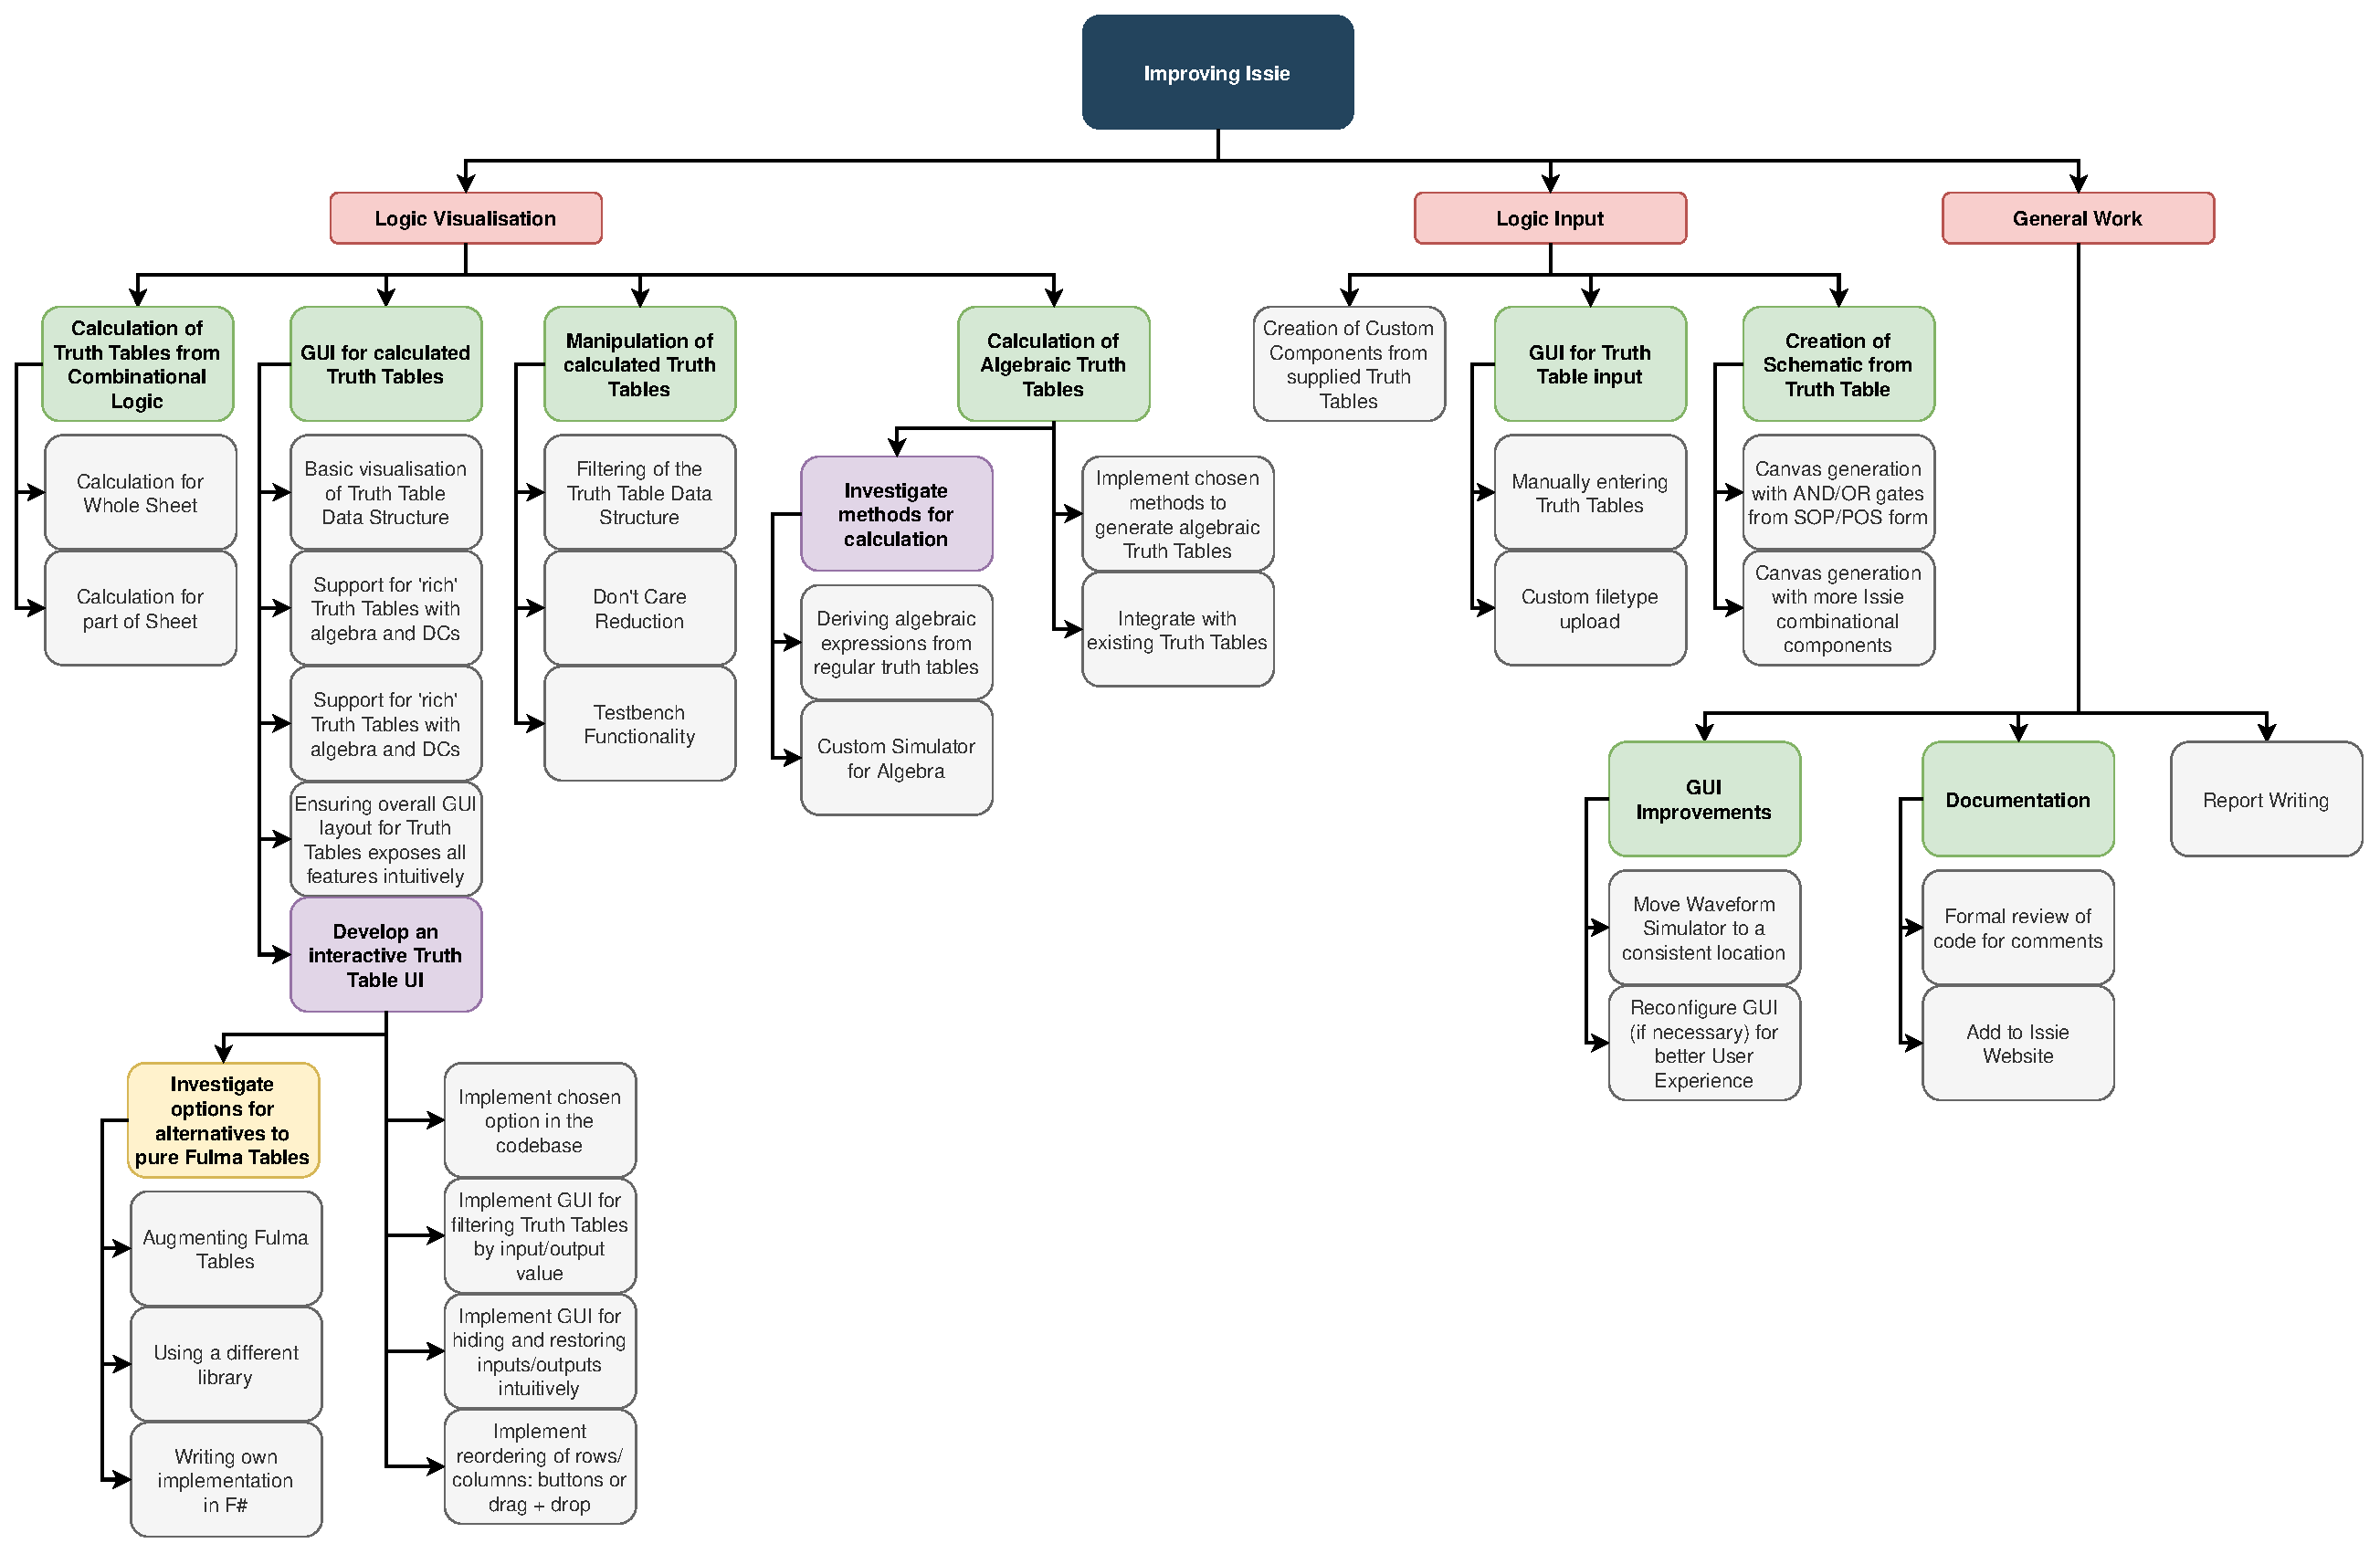
\includegraphics[width=22cm,angle=270,origin=c]{05.ImpPlan/wbs.eps}
    \caption{Work Breakdown Structure for the Project (Rotated)}
    \label{fig:wbs}
\end{figure}

\begin{figure}
    \centering
    \includegraphics*[width=\textwidth]{05.ImpPlan/gantt_update.pdf}
    \caption{Gantt Chart for the Project}
    \label{fig:gantt}
\end{figure}
\chapter{Testing and Results}
The delivered improved version of Issie was tested from three perspectives. These were \textbf{correctness}, \textbf{performance}, and \textbf{user experience}. Testing the correctness of the improvements made to Issie included checking that the implemented functionality worked as intended, as well as ensuring that the application was stable, not crashing regardless of user input. Quantitative performance testing was conducted by first measuring the average time taken for specific actions and processes, and then those measurements to Robert Miller's \cite{Miller1968ResponseTI} classes for perceived responsiveness of an application. Finally, the quality of the user experience was evaluated by giving survey participants a series of tasks in Issie, measuring their performance, and collecting their feedback.

\section{Testing Application Stability} \label{sec:testappstability}
An application is considered stable when the user is not subjected to undefined behaviour or inexplicable crashes while using the application. The stability of the improved version of Issie delivered by the project was verified by analysing cases in the codebase which could trigger a system crash, and systematically evaluating that they could not occur. There are two scenarios which can cause Issie to crash:
\begin{itemize}
    \item Un-handled exceptions: exceptions can either be generated by the developer or can be generated by library functions. If these exceptions are not caught and handled appropriately, the cause the application to crash.
    \item When \codestyle{failwithf} is called in the code: this function is called when an unexpected case that should never occur is matched in the code. An example of this would be if the Update function receives the instruction to reduce a truth table with Don't Cares when no truth table exists.
\end{itemize}

\subsection{Exception Analysis}
The code added to Issie was analysed to explore the scenarios in which exceptions could be raised. Exceptions are uncommon in F\fsharp -- instead the use of Monad types such as \codestyle{Option} and \codestyle{Result} is preferred. When using Monad types, failure of an operation is an option and the programmer is made to account for the possibility of it while programming. In contrast, functions which return exceptions place the onus of verifying the arguments prior to the call on the developer. An example of this is the difference between the functions \codestyle{Map.find} and \codestyle{Map.tryFind}; both functions look up a key in a Map and return the corresponding value, but return the value in different ways. When a key exists, \codestyle{Map.find} returns the value, but when it does not exist it raises an exception. If the developer fails to account for this, the program may crash unexpectedly. In contrast \codestyle{Map.tryFind} wraps the returned value in the \codestyle{Option} type, and returns \codestyle{Some value} if the key exists in the Map, or \codestyle{None}. Therefore, when using \codestyle{Map.tryFind}, the developer must always actively handle the failure case at that point in the code, either providing alternate behaviour or manually making the choice to fail the application with \codestyle{failwithf}. This significantly reduces the chance of application crashes due to an oversight made by the developer with regard to exception handling. 

All library functions used in the code written during the project were analysed, and it was checked which of the ones used could possibly return any exceptions. For each of these functions a strategy was devised to check whether an exception could occur in practice:

\begin{table}[ht]
    \centering
    \begin{tabular}{|m{3cm}|m{9cm}|m{2cm}|}
    \hline
        Function &  Check & Pass/Fail\\ \hline
        \codestyle{List.except} & Ensure that the items to exclude sequence can never be null. & Pass \\\hline
        
        \codestyle{List.head} & Ensure that the supplied list is not empty either through a conditional statement or pattern match case on the list. & Pass \\ \hline
        
        \codestyle{List.updateAt} & Ensure that the index is valid (between 0 and length-1) either through a bounds check or from properties. & Pass \\ \hline
        
        \codestyle{Seq.allPairs} & Ensure that the both sequences can never be null. & Pass \\\hline
        
        \codestyle{Seq.append} & Ensure that the both sequences can never be null. & Pass \\\hline
        
        \codestyle{Seq.init} & Ensure that the count can never be negative. & Pass \\\hline
        
    \end{tabular}
    \caption{Library functions in project code which can throw exceptions}
    \label{tab:exceptions}
\end{table}

Exceptions can also be raised in the code by the developer if required, and caught using a \codestyle{try-catch} block. This project only adds one such exception; the \codestyle{AlgebraNotImplemented} exception which is be raised in the Fast Simulation function \codestyle{fastReduce} when algebra is passed to an unsupported port or component. An exception is used here because manually propogating a \codestyle{SimulationError} up the call stack would be very impractical. The \codestyle{AlgebraNotImplemented} exception contains a \codestyle{SimulationError} data structure; whenever there is a scenario in which algebra is fed to the Fast Simulation, there is a \codestyle{catch} block waiting to catch any the exception and return the \codestyle{SimulationError} contained within. Additionally, the XML documentation of functions in the Fast Simulator has been updated to reflect the new exception. Therefore, it can be said that the code added by this project to Issie is stable from an exception point-of-view.

\subsection{Failure Analysis}
To ensure that the application could not fail during use, every \codestyle{failwithf} case in the project code was inspected, and a summary made of the scenarios in which the function would be called. Once the scenario was ascertained, one of two actions woere taken. If the fail case was related to application state, it was ensured through thorough inspection of the code that such a state could never occur. If the fail case was related to the UI, testing involved attempting to create those circumstances in the application. In all cases, attempts to achieve scenarios that would call the application to fail and exit were unsuccessful. 

In addition to exception and failure analysis, the completed application has been used for other purposes for long periods of time. The process of repeatedly testing the correctness of other features totalled over 3 hours, in which multiple tasks were carried out using the application. Additionally, during user experience testing, not a single user reported any crashes or undefined behaviour. This supports the notion that the code added to the project is robust and stable, and that all situations with erroneous user input have been handled.

\section{Correctness Testing}
Correctness of the implemented features was tested by testing the features on 6 different circuits, each of varying complexity. These circuits can be described as:
\begin{itemize}
    \item A two-input multiplexer circuit implemented only using gates
    \item A circuit containing a Mux4 component with 2-bit inputs to each data line of the multiplexer
    \item A circuit which calculates the bitwise And of two 8-bit inputs
    \item A Full Adder circuit using a Half Adder custom component, all built exclusively from logic gates
    \item A circuit which either adds or subtracts two 16-bit values depending on the selected mode
    \item An 8-bit ALU, which is a custom component in the design of an 8-bit CPU
    \item An 8-bit CPU design
\end{itemize}

A summary of the tested features can be found in Table \ref{tab:test}. All of the tested features worked as intended for all schematics, indicating that they have been implemented correctly and will therefore work reliably when distributed to real-world users.

\begin{longtblr}[
  caption = {List of all features which were manually tested},
  label = {tab:test},
]{
  colspec = {|X[5]|X|},
  rowhead = 1,
  hlines,
} 
\textbf{Feature Checked} & \textbf{Pass/Fail} \\
For all combinational circuits, a numeric truth table can be generated for the whole sheet.  & Pass \\
For all valid selections of a schematic, a numeric truth table can be generated:
\begin{enumerate}
        \item The selected canvas is corrected successfully, with newly generated input or output components.
        \item Newly generated IOs are labelled based on which component ports they connect to.
        \item Truth tables for selections can be generated even if errors or sequential components exist elsewhere in the schematic.
    \end{enumerate} & Pass \\
If there are errors in the schematic, the \textit{See Problems} button appears in place of the \textit{Generate Truth Table} button, and clicking it conveys the error to the user.  & Pass \\
Users are prevented from generating truth tables for schematics containing sequential logic, and this reason is conveyed to them. & Pass \\
For all circuits where the total width of all the inputs combined exceeds 10 bits, a truncated truth table of 1024 rows is displayed, along with a warning notification informing the user about the truncation.  & Pass \\
The base of numbers in the truth table can be changed using the base selector.  & Pass \\
Truth table related functionality can be shown and hidden by expanding and closing menu sections.  & Pass \\
Input constraints can be applied to the truth table and successfully change the input state so that rows that were previously truncated are now generated and displayed.  & Pass \\
Significantly restrictive input constraints will reduce the input space enough so the truth table will no longer be truncated.  & Pass \\
Output constraints filter the existing truth table.  & Pass \\
There is an intuitive interface for adding/removing constraints:
\begin{enumerate}
    \item Clicking on the \textit{Add} button opens the constraint editor popup.
    \item Changing the chosen IO in the IO selection section updates the IO displayed in the editor section.
    \item Real-time validation of constraints is performed as they are entered, with errors clearly conveyed to the user.
    \item Constraints that are currently being applied are clearly displayed to the user with tags, and can be deleted easily by clicking the cross next to them.
    \item All constraints can be cleared in one go with the \textit{Clear All} button.
\end{enumerate} & Pass \\
Columns in the truth table can be hidden by using the column hider toggles.  & Pass \\
Rows in the truth table can be sorted based on a chosen IO, in ascending and descending order.  & Pass \\
The sorting information is conveyed to the user successfully through the highlighting of the relevant sorting arrow.  & Pass \\
The order of columns in the truth table can be changed.  & Pass \\
Non-truncated truth tables can be reduced with Don't Cares, with the resultant table containing no redundant rows.  & Pass \\
Users are prevented from DC reducing truncated truth tables.  & Pass \\
Users can change some or all inputs to algebra in the truth table:  
\begin{enumerate}
    \item Clicking the algebra button always spawns the algebra selector popup, where inputs can be toggled between numeric and algebraic values.
    \item If a certain input is not supported as being algebraic, the user is informed of the reason why. They are prevented from applying the incompatible algebraic inputs.
    \item When algebraic inputs are in the truth table, the outputs are informative algebraic expressions which is a correct function of the inputs.
\end{enumerate} & Pass \\
Algebraic reduction rules are applied correctly, yielding correctly simplified algebraic expressions at the outputs  & Pass \\
Algebraic expressions are printed correctly in the truth table.  & Pass \\
When the truth table tab is open, width of the right section can be changed using the draggable dividerbar.  & Pass \\
The truth table is responsive:
\begin{enumerate}
    \item Changing the width of the right section changes the width of the truth table (therefore of the columns in the table).
    \item When the content inside a truth table cell is too wide, the height of the row automatically adjusts so that the content can wrap to the next line.
    \item Operations on the truth table appear instantaneous.
\end{enumerate} & Pass \\
The waveform simulation can successfully be run from the new Waveform Simulator sub-tab.  & Pass \\
\end{longtblr}

\section{Quantitative Performance Testing} \label{sec:performance}
The three following schematics were used for measuring the performance of the application, with each having slightly different attributes. All tests were performed on a MacBook Air, featuring an M1 CPU with 8GB of RAM.
\begin{enumerate}
    \item A circuit containing a Mux4 component with 2-bit inputs to each data line of the multiplexer. In total, this circuit has 5 2-bit inputs, meaning that it will generate exactly 1024 rows (no truncation required). This is a simple circuit with only one component, so should be quick to simulate. However, there are many redundancies in the truth table, so Don't Care reduction may take longer.
    \item A circuit which either adds or subtracts two 16-bit values depending on the selected mode. This circuit features slightly more complex logic than the previous one, and also will result in the truth table being truncated. This will be referred to as the 'Add Or Sub' schematic.
    \item An 8-bit ALU, which is a very complex schematic featuring lots of library and custom components. This should test the generation algorithm to the maximum.
\end{enumerate}

\subsection{Generating Numeric Truth Tables}
The time taken to generate a numeric truth table was measured for all three aforementioned schematics.
\begin{table}[!ht]
    \centering
    \begin{tabular}{|l|l|l|l|l|l|l|}
    \hline
        Sheet & Trial 1 & Trial 2 & Trial 3 & Trial 4 & Trial 5 & Average \\ \hline
        Mux4 & 52 & 58 & 51 & 49 & 51 & 52.2 \\ \hline
        Add Or Sub & 75 & 72 & 69 & 81 & 78 & 75 \\ \hline
        ALU & 697 & 702 & 700 & 697 & 702 & 699.6 \\ \hline
    \end{tabular}
    \caption{Time taken to generate a numeric truth table (ms)}
    \label{tab:timeTT}
\end{table}

\subsection{Algebraic Truth Tables}
The time taken to calculate an algebraic truth table for the 8-bit ALU was measured. The circuit had five inputs in total: A and B which were 8 bits, X and F which were 3 bits, and Cin which was 1 bit. A, B, and Cin were set as algebraic inputs for the experiment. Five trials were carried out, and the average time was calculated. 

\begin{table}[!ht]
    \centering
    \begin{tabular}{|l|l|l|l|l|l|}
    \hline
        Trial 1 & Trial 2 & Trial 3 & Trial 4 & Trial 5 & Average \\ \hline
        45 & 42 & 44 & 47 & 45 & 44.6\\ \hline
    \end{tabular}
    \caption{Time taken to generate an algebraic truth table for the ALU schematic (ms)}
    \label{tab:timeAlgTT}
\end{table}

\subsection{Don't Care Reduction}
The time taken to reduce an existing truth table using Don't Cares was measured for two schematics. The Mux4 schematic was first tested, as it contains multiple redundancies and therefore requires repeated rounds of reduction. Secondly, the 'Add Or Sub' schematic was tested. As this schematic exceeds the bit limit, the input space was limited; inputs A and B were constrained to between 0 and 16. This schematic was chosen as there are no redundant rows in the truth table, as every input contributes to the output. This represents a scenario in which no DC rows are valid, and therefore the process will stop after one round of attempted reduction.

\begin{table}[!ht]
    \centering
    \begin{tabular}{|l|l|l|l|l|l|l|}
    \hline
        Sheet & Trial 1 & Trial 2 & Trial 3 & Trial 4 & Trial 5 & Average \\ \hline
        Mux4 & 2590 & 2586 & 2589 & 2616 & 2598 & 2595.8 \\ \hline
        Add Or Sub & 265 & 263 & 260 & 259 & 263 & 262 \\ \hline
    \end{tabular}
    \caption{Time taken to reduce a numeric truth table using Don't Cares (ms)}
    \label{tab:timeDCTT}
\end{table}

\subsection{Graphical Manipulation of Truth Tables}
Using the truth table generated for the ALU schematic, the time taken to perform three graphical manipulations was measured. These manipulations were: hiding an output column, sorting the truth table, and moving a column. The ALU schematic was chosen as it will generate a truncated truth table, meaning that the maximum possible 1024 rows will be rendered. It also contains 8 IOs, which is a sizeable amount.

\begin{table}[!ht]
    \centering
    \begin{tabular}{|l|l|l|l|l|l|l|}
    \hline
        Operation & Trial 1 & Trial 2 & Trial 3 & Trial 4 & Trial 5 & Average \\ \hline
        Sorting Truth Table & 35 & 33 & 36 & 41 & 39 & 36.8 \\ \hline
        Moving a Column & 21 & 25 & 22 & 23 & 27 & 23.6 \\ \hline
        Hiding a Column & 43 & 38 & 37 & 39 & 38 & 39 \\ \hline
    \end{tabular}
    \caption{Time taken to conduct different graphical manipulations on a truth table (ms)}
    \label{tab:timeTTManip}
\end{table}

\section{User Experience Testing} \label{sec:uxtest}
The success and long-term viability of any user-facing application or platform is highly dependent on the user experience it provides. For this reason, feedback must be collected from users to evaluate whether the application is achieves its purpose, and whether it if user-friendly. User feedback was collected to answer the following questions:
\begin{enumerate}
    \item Do the added features fulfil the project aim, which is to add effective novel ways of visualising combinational logic in Issie, delivering an improved education and hardware design platform?
    \item Are these features implemented in a user-friendly manner?
\end{enumerate}

The participants of the user feedback survey consisted of a group of 12 engineering students across multiple departments at Imperial College, most of whom had some beginner-level experience with combinational logic design. Participants were chosen this way so that they would not be confused by the digital electronics concepts, and would therefore be able to fully appreciate and use the added functionality. The feedback collection process consisted of two stages; in the first stage participants were provided with the updated version of Issie, then tasked with investigating five 'mystery' Issie sheets and summarising the logical function implemented by each. They were asked to use the truth table functionality while doing so, but were not pointed to where it was located in the application. The second stage consisted of a questionnaire, in which participants were given the opportunity to evaluate their experience using Issie.

\subsection{Stage 1: Mystery Sheets}
Participants were provided with five schematics labelled \textit{mystery1} to \textit{mystery5}, and were asked to describe what each sheet did. While the instructions encouraged them to "use truth tables and other features in the Truth Tables tab", they were not told where this tab was in the app's top-level UI, nor were they instructed on how to use any of the features. This was done on purpose as Issie meant to be easy to use without explicit guidance. Through this the \textit{intuitiveness} and \textit{obviousness} of the UI for truth tables was tested. The mystery sheets increased in complexity, with the initial sheets being simple to introduce the user to the application, and later sheets being more complex to push the user to explore more and use many of the added features. Table \ref{tab:mystery} provides a summary of each mystery sheet, as well as the rationale behind using it in the survey. The purpose of this exercise was to ascertain whether the added features did indeed help users gain a better understanding of combinational logic designs. Sheets Mystery 1 to Mystery 4 had a perfect record, while only one user failed to understand what Mystery 5 was doing.

\subsection{Stage 2: Questionnaire}
Once the participants had a chance to use Issie's truth table features, they were asked a series of questions about their experience. These questions fell into two categories. In the first section, they were presented with a five statements and asked to respond to them ranking them on a scale of 1 - 5, with 1 corresponding to "Strongly Disagree" and 5 corresponding to "Strongly Agree". The aim of this part of the questionnaire was to judge the quality of the user experience from different angles. The responses to this first set of questions were aggregated into a score by taking the average. Table \ref{tab:strongqs} shows the score for each statement, as well as the rationale behind why the statement was included in the questionnaire.

The second set of questions in the questionnaire focused on determining the discoverability of the implemented features. Features in an application are only useful if they are discovered by the user, so observing which features are found is important. In addition to asking whether a named feature was found, the questions also asked if they found the feature useful. The rates of discovery and usefulness -- i.e. the percentage of participants who discovered the features and found them useful, is shown in Figure \ref{fig:discgraph}.

\begin{table}[h]
    \centering
    \begin{tabular}{|m{4.2cm}|m{7cm}|m{2cm}|}
    \hline
        \textbf{Diagram} & \textbf{Explanation of Mystery Sheet} & \textbf{Score} \\
        \hline
        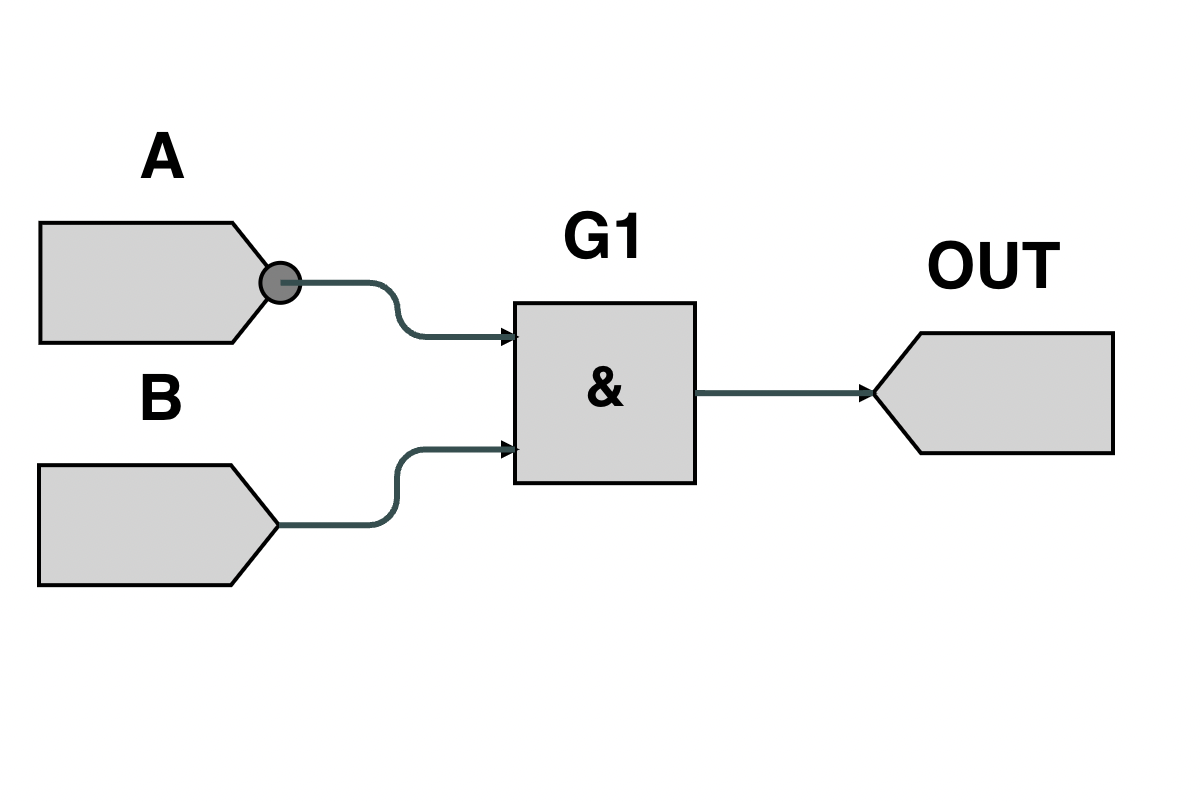
\includegraphics[width=4cm]{06.TestRes/m1.png} & \textbf{Mystery 1: Simple And Gate} The first mystery sheet was intentionally made very easy. This was done to allow users to familiarise themselves with the application and the truth table generation method. The truth table for an AND gate is very basic and is one of the first things engineering students learn. The idea was that participants would be able to use this as a reference to understand the look and feel of truth tables in Issie. & 100\% \\ \hline
        
        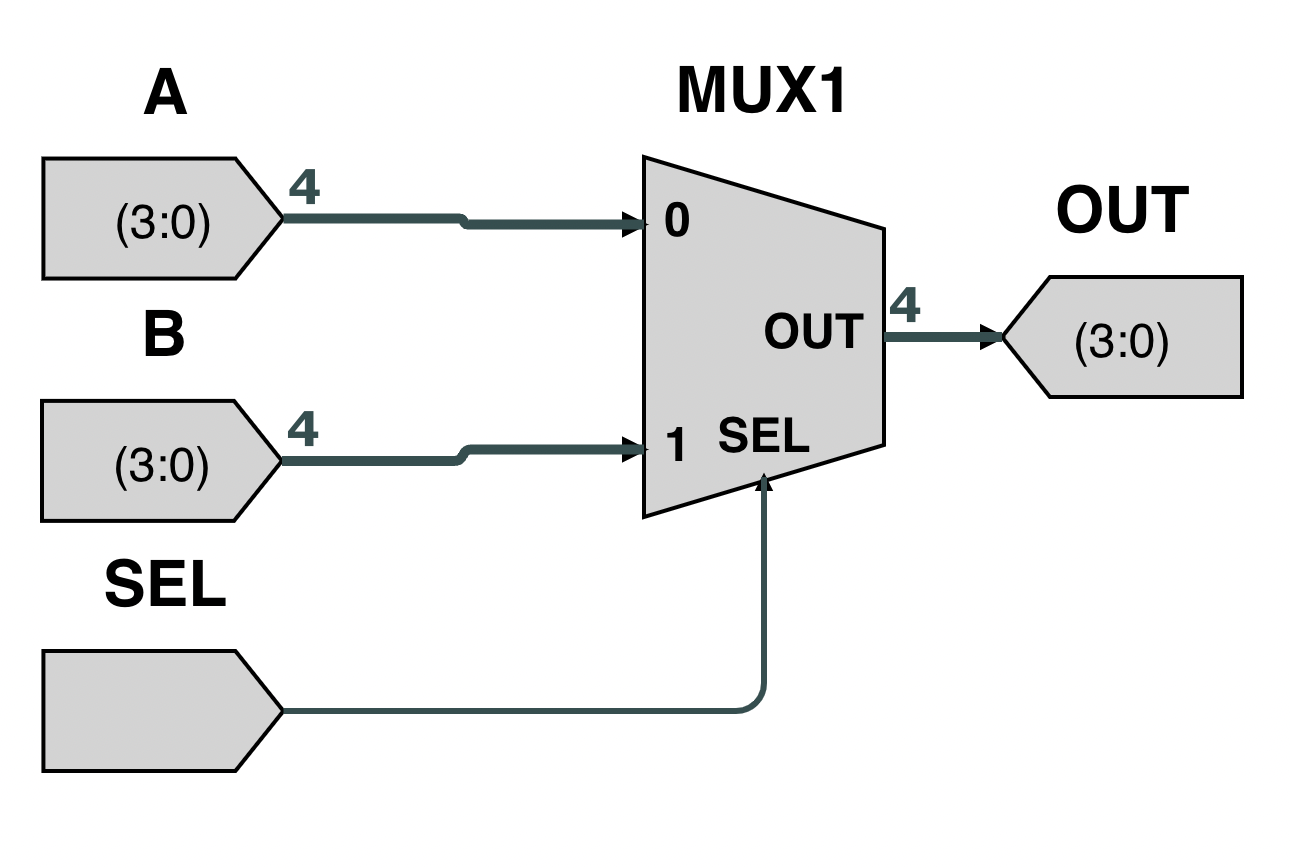
\includegraphics[width=4cm]{06.TestRes/m2.png}& \textbf{Mystery 2: Multiplexer} The second mystery sheet features a single MUX2 component which takes multi-bit inputs. This circuit was chosen as it exposes the user to truth tables which contain numbers other than 0 and 1. It also lets them DC Reduce the truth table, making it clear that B does not matter when SEL is 0, and A does not matter when SEL is 1. & 100\% \\
         \hline
         
         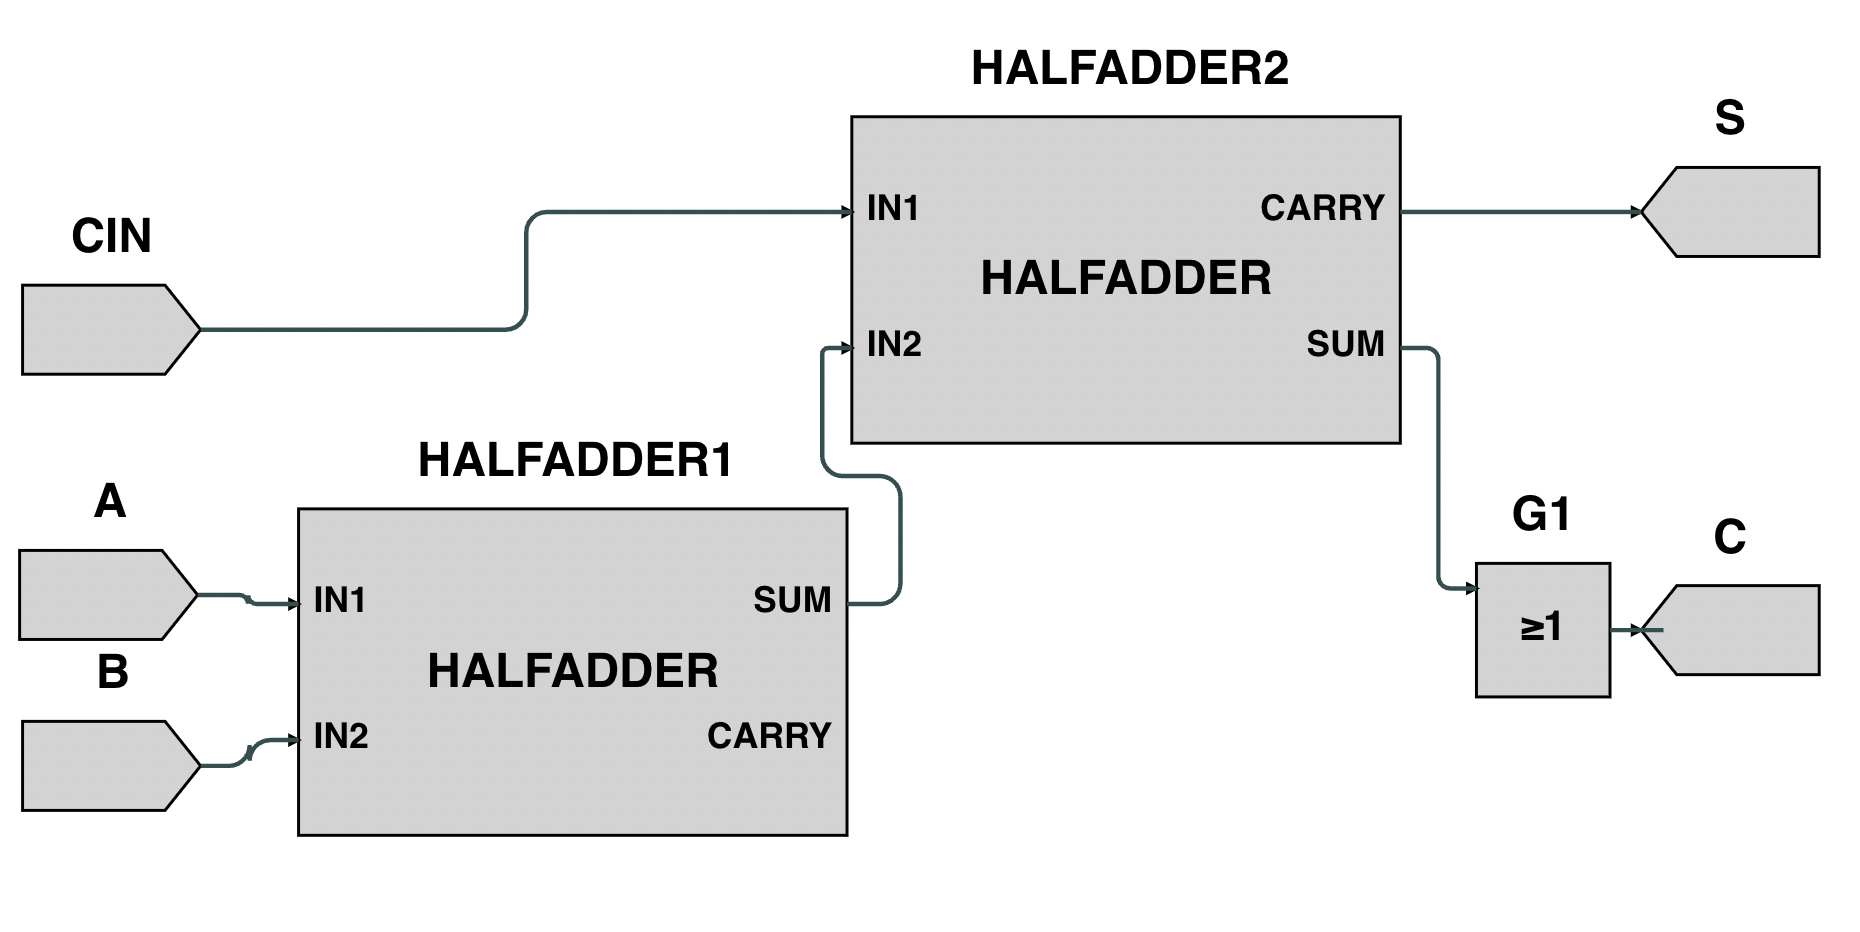
\includegraphics[width=4cm]{06.TestRes/m3.png}& \textbf{Mystery 3: Full Adder} The third mystery sheet is a full adder, which uses half adders custom components. Users can generate a truth table for the half adder alone by selecting it. This schematic also allows the user to explore algebraic reduction, as the arithmetic relationship can be inferred from the truth table. & 100\% \\
         \hline
         
         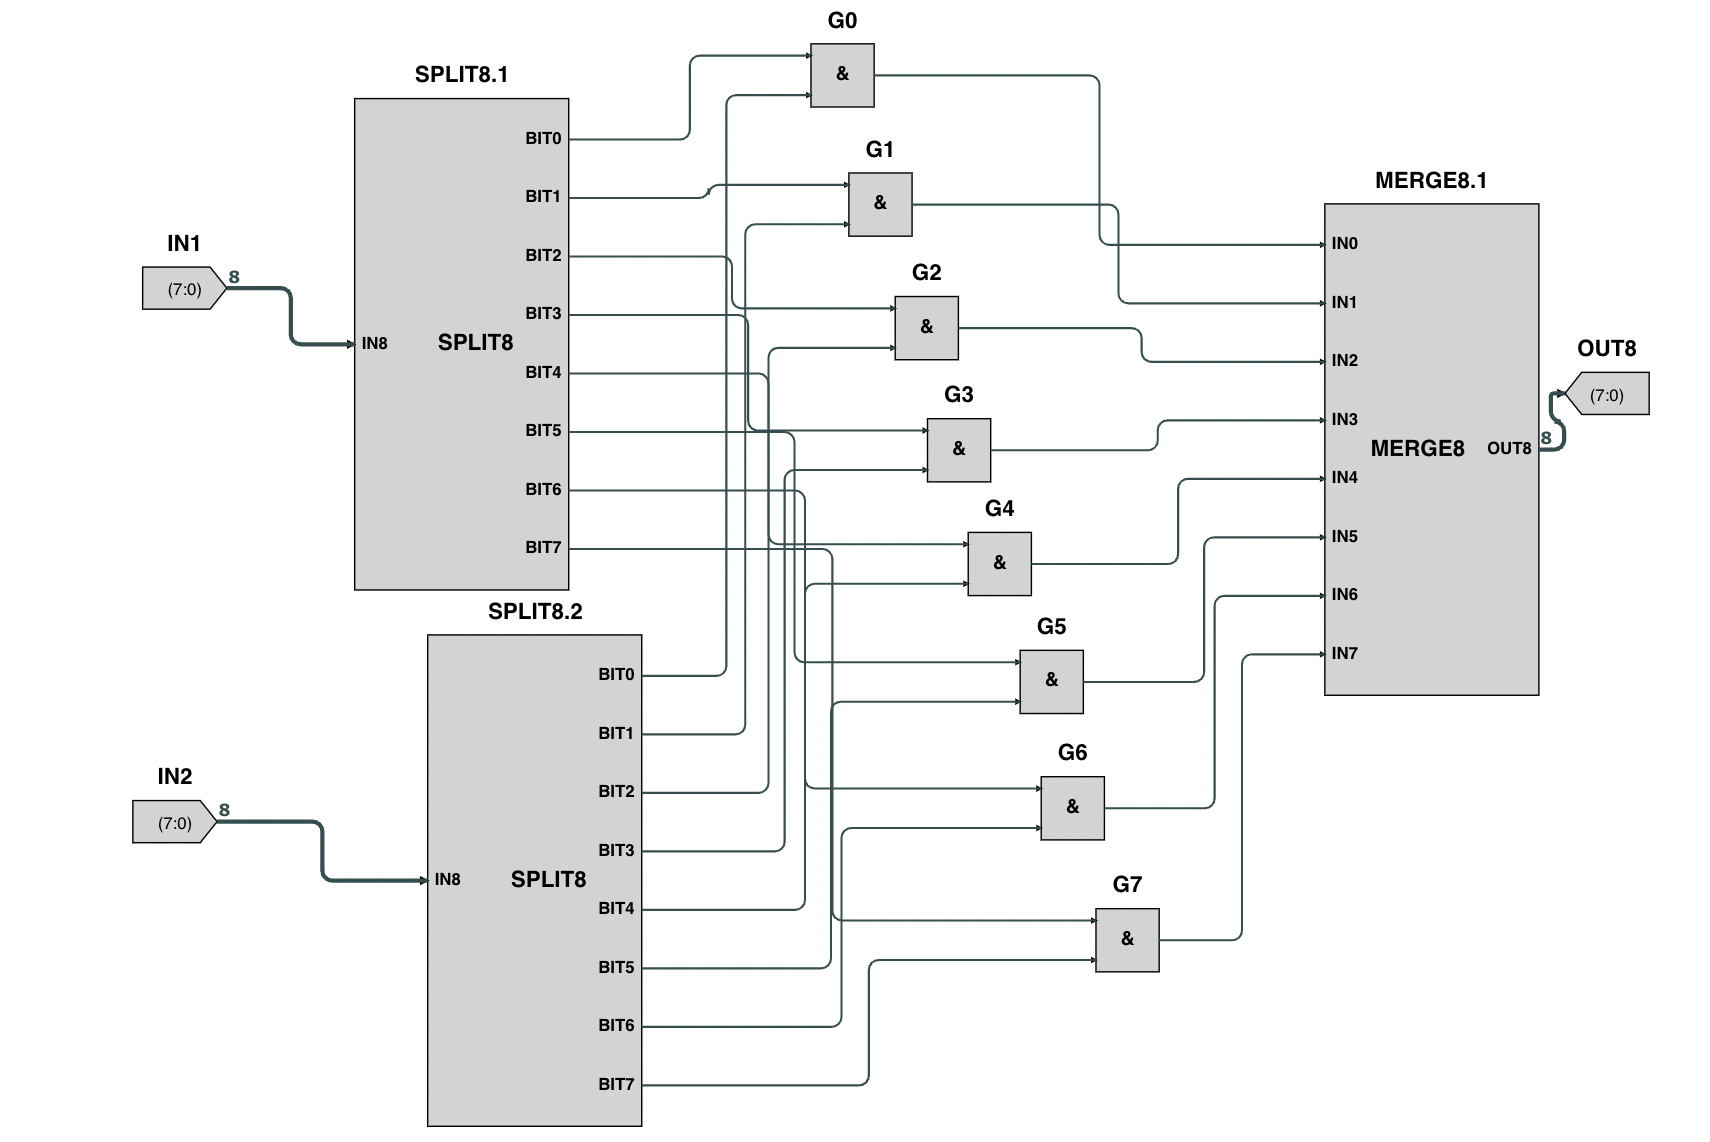
\includegraphics[width=4cm]{06.TestRes/m4.png}& \textbf{Mystery 4: Bitwise And} The fourth mystery sheet contains a large schematic with custom components and multiple wires. Such a schematic can be difficult to understand simply by looking at it. In contrast, algebraic reduction in the truth table identifies the schematic as being a simple bitwise And betwen the two inputs. & 100\% \\
         \hline
         
          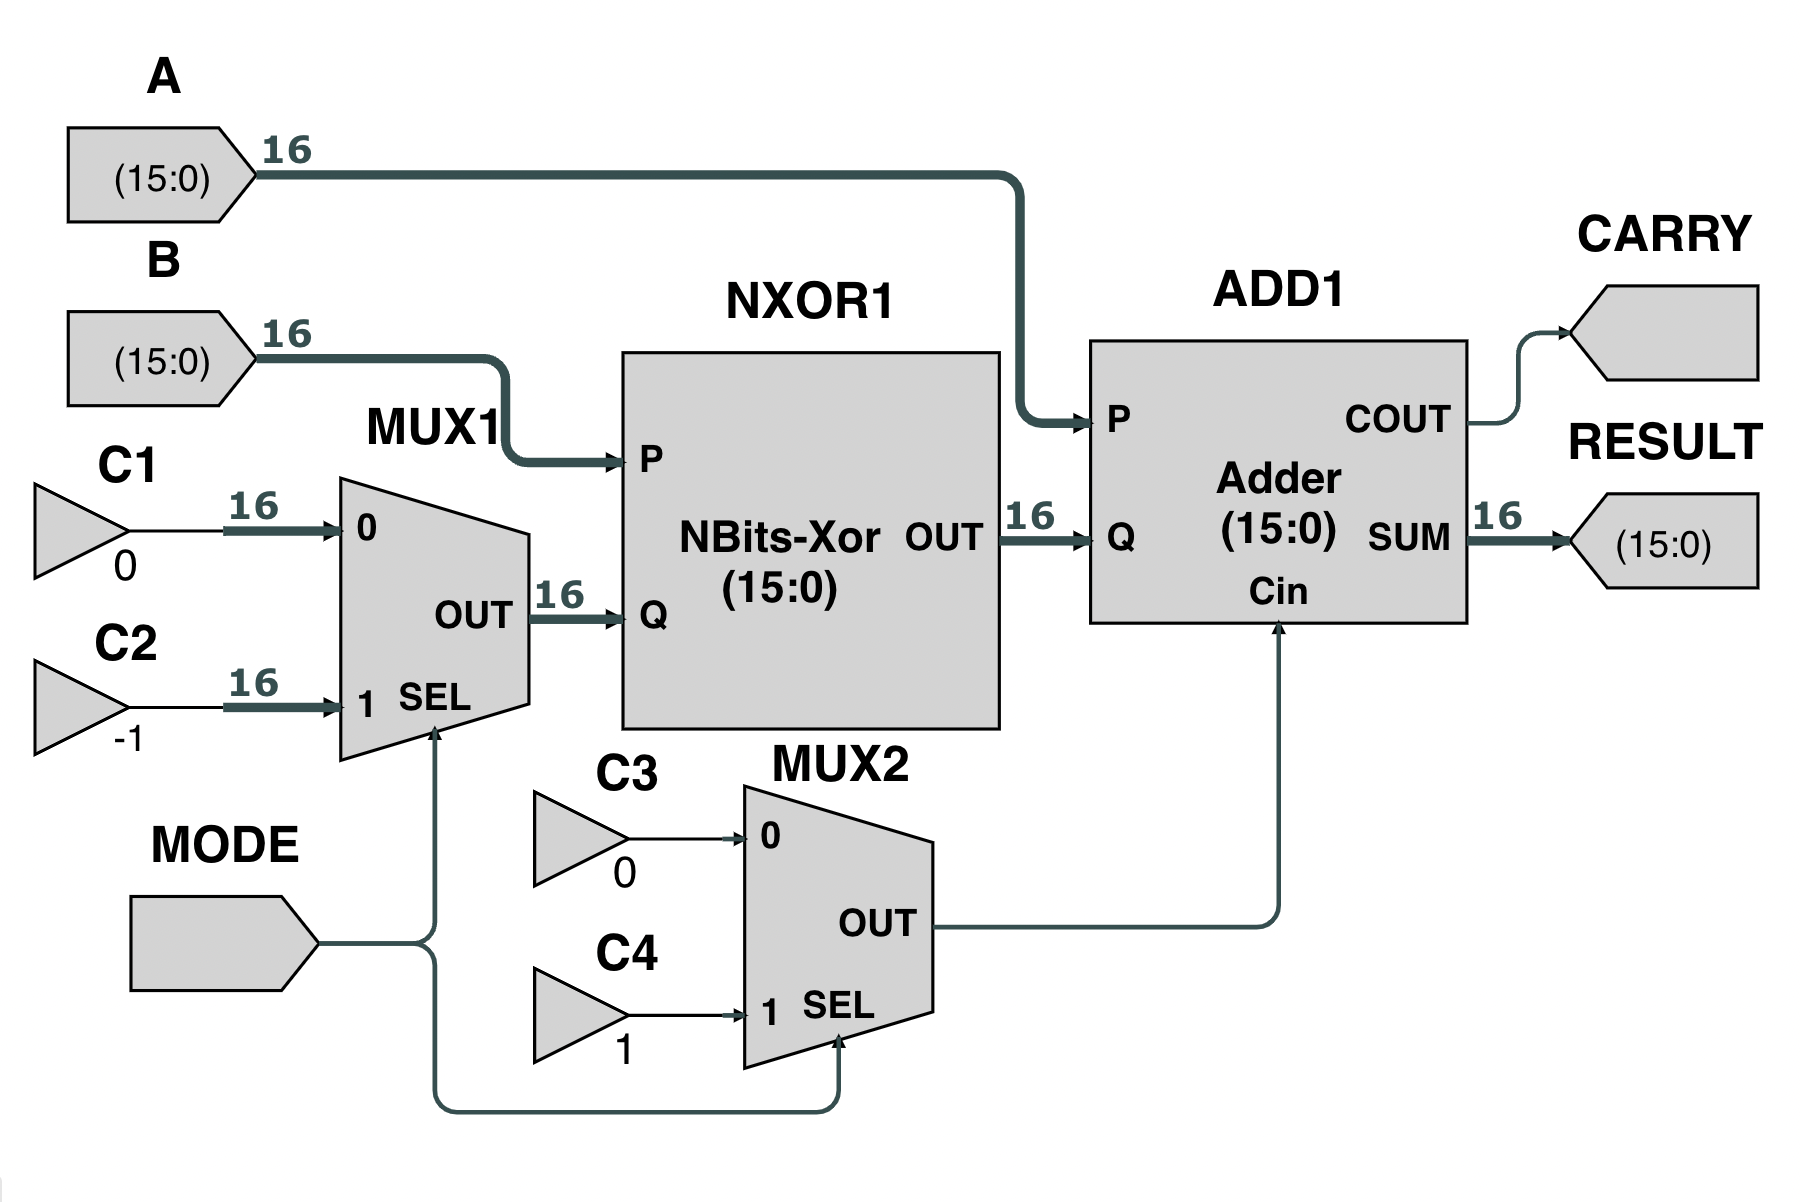
\includegraphics[width=4cm]{06.TestRes/m5.png}& \textbf{Mystery 5: Addition or Subtraction} The fifth mystery sheet incorporates Issie's built-in arithmetic components; the N-bit Adder and the N-bit XOR. The MODE input controls whether the circuit adds the two inputs, or subtracts one from the other. This circuit is more complex than the previous mystery circuits, and the inputs A and B are both 16 bits wide. This introduces the user to truth table truncation. However, using algebra, the function of the circuit can be discovered. & 90.1\% \\
         \hline
    \end{tabular}
    \caption{Mystery Sheets}
    \label{tab:mystery}
\end{table}

\begin{table}[t]
    \centering
    \begin{tabular}{|m{5cm}|m{5.5cm}|c|}
    \hline
        \textbf{Statement} & \textbf{Rationale} & \textbf{Average Score} \\ \hline
        Finding the Truth Table tab in Issie's top-level UI was easy & Evaluates the top-level UI redesign of the application. If the user can find the truth table tab easily, this means that they will likely be able to find all simulation activities. & 4.45 \\ \hline
        The functionality related to Truth Tables is clear and obvious in the UI. & Obviousness is a core principle of Issie, so evaluating whether the added features are presented in a way such that they are easy to find and understand. & 4.63 \\ 
        \hline
        Once I found a feature, it was easy to figure out what it did and how to use it. & Intuitiveness is a core principle of Issie, and this question aims to evaluate how easily the user can intuitively understand what features do. & 4.45 \\ \hline
        Using truth tables made it easier to understand the relationship between inputs and outputs in combinational logic compared to looking at the schematic. & Evaluates the effectiveness of the truth table feature set as a whole in improving the visualisation of combinational logic in Issie. & 4.36 \\ \hline
        The algebraic expressions in the truth table make it easy to understand the intended function of the circuit. & Evaluates the effectiveness of the algebraic expressions in particular for clearly communicating what the circuit does. & 4.54 \\ \hline
    \end{tabular}
    \caption{First set of questions asked in questionnaire}
    \label{tab:strongqs}
\end{table}

\begin{figure}[b]
    \centering
    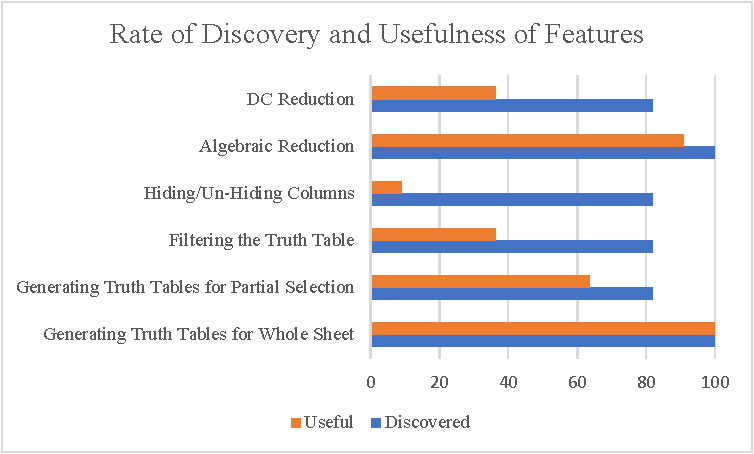
\includegraphics[width=\textwidth]{06.TestRes/graph.pdf}
    \caption{Graph showing the percentage of participants which discovered each feature and found it useful}
    \label{fig:discgraph}
\end{figure}


\section{Testing on the 8-bit ALU} \label{sec:alu}
To evaluate both the usefulness and correctness of the new combinational logic visualisation methods added to Issie, an 8- bit ALU was was analysed using the added features.
The schematic diagram of this ALU can be found in Figure \ref{fig:alu8bit} in Appendix \ref{app:alu}. The inputs into the schematic have a total width of 23 bits, yielding a theoretical truth table size of over 8 million rows. The truth table is generated in under 1 second, but truncated to 1024 rows. Due to its size, and given that the exact specification of the ALU was not known at that point, the numeric truth table was not massively useful. However, had the specification been known prior to analysis, the numeric truth table would have undoubtedly been useful for checking the correctness of multiple input/output combinations. In order to further understand the ALU functions, algebraic reduction was used. The inputs $A$, $B$, and $CIN$ were set as algebra; this reduced the truth table size from over 8 million rows to 64. The first 18 rows of this algebraic truth table can be seen in Figure \ref{fig:alutable}. The other inputs, $X$ and $F$, eventually propagate to the SEL ports of multiplexers and therefore cannot be set as algebra. However, this works out very well -- these inputs control the behaviour of the ALU, meaning that it is better for their values to stay as numbers in the truth table. For each combination of these control inputs, a different expression at the output of the ALU ($OUT$) can be observed. From the algebraic truth table, the logical function of the ALU was described using eight short statements:
\begin{enumerate}
    \item When $X = 0$ and $F = 0$, $OUT$ is the sum of A and B
    \item When $X = 0$ and $F = 2$, $OUT = A - B$
    \item When $X = 0$ and $F = 6$, $OUT = CIN + A - B$
    \item When $X = 0$ and $F = 4$, $OUT$ is the sum of A, B, and CIN
    \item When $X = 0$ and $F[0] = 1$ (i.e. F is odd), $OUT = B$
    \item When $X = 1$, $OUT = A \& B$
    \item When $X = 2$ or $X = 3$, $OUT$ is the XOR of A and B
    \item Otherwise, $OUT$ is $B$ right-shifted by 1.
\end{enumerate}

\begin{figure}
    \centering
    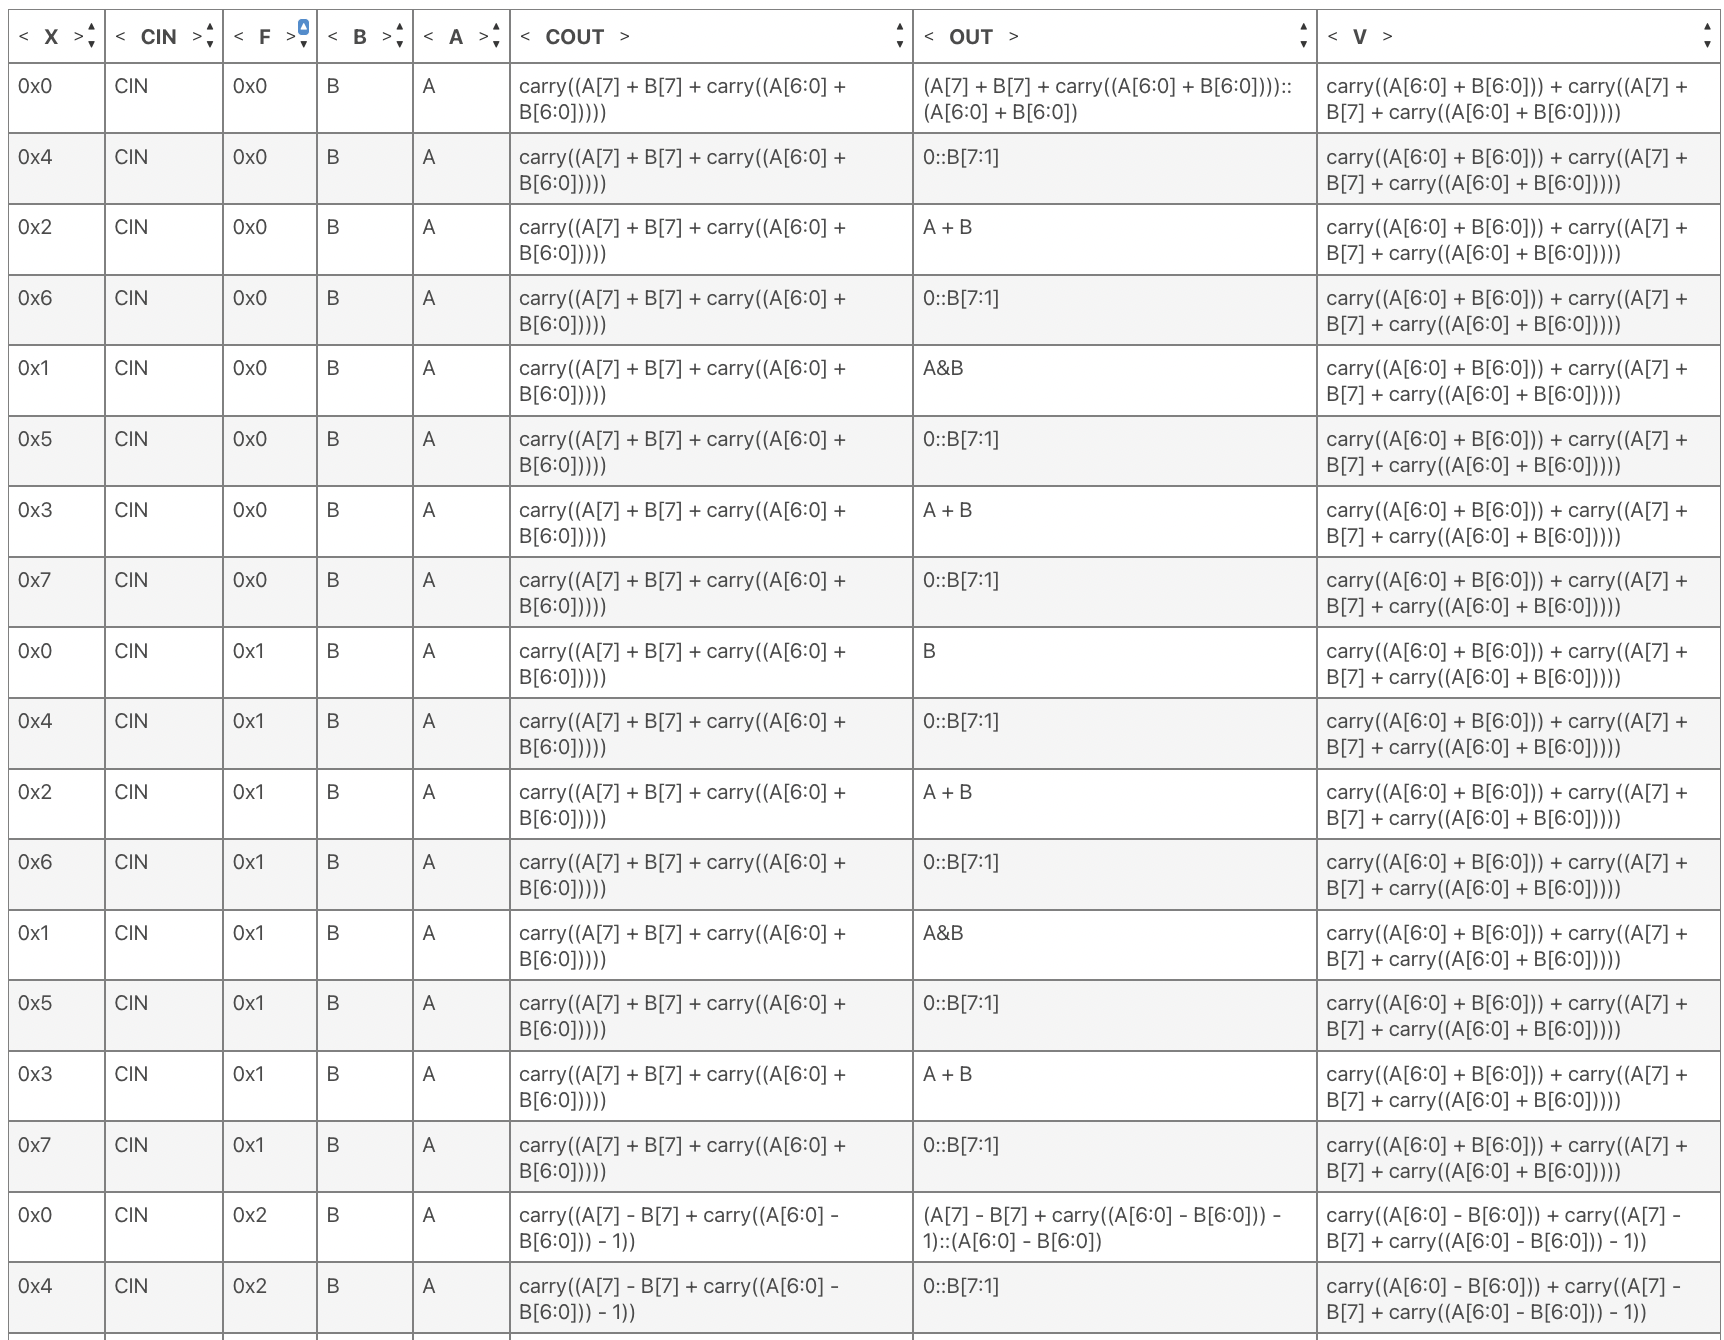
\includegraphics[width=\textwidth]{06.TestRes/alutable.png}
    \caption{First 18 rows of the Algebraic Truth Table for 8-bit ALU}
    \label{fig:alutable}
\end{figure}
\chapter{Evaluation}
In Chapter \ref{chap:intro}, the key aims for the project were established, and using these the project was defined. This chapter will evaluate whether these aims and deliverables have been met through a variety of methods. From these aims, a set of formal requirements were defined in Chapter \ref{chap:requirements}, describing in detail what the project must complete in order to be considered successful. This chapter evaluates the final project deliverable against the aforementioned aims and requirements. This is done through a variety of methods, including evaluation against Issie's core principles, evaluation of key functionality in the application, analysis of performance data, as well as interpretation of user feedback. 

\section{Evaluation against Project Aims}
The principal aim of the project was to explore novel ways in which interactivity could be added to automatic schematic-derived truth tables, and how these could be used as a fast aid to design combinational logic. Alongside the research, the main deliverable was stated as an updated version of Issie which featured these interactive truth tables. Additionally, an overarching aim was defined for the project; improving Issie in such a way that it is easier for students to understand the use of combinational logic in digital design. This section evaluates the improved version of Issie delivered by this project against these aims, ultimately concluding whether or not the aims were fulfilled.

Automatic schematic derived truth tables have been implemented using repeated simulation of the schematic. These truth tables are generated through repeated simulation of all input combinations, with the whole process taking under 1 second. A caveat on these schematic-derived truth tables is that they can only handle an input space 10 bits wide, placing a limit of 1024 rows on truth table size. While this is a theoretical limitation, as discussed during the design of the system, in practice it is unlikely that any user would be able to effectively comprehend a truth table of such a large size anyways. Additionally, the user has the option to re-generate the truth table with a tighter set of input constraints or with algebraic inputs to gain a more informative truth table. Both of these are examples of where \textit{interactivity} has been added to the original schematic-derived truth table. Using input constraints, users can limit the input space and find/verify patterns in the resultant outputs. Seeing all the cases in a well-formatted list is more convenient than having to repeatedly run simulations and remember the result. Output constraints enable the reverse; users can specify a set of outputs and see which inputs into the logic cause them to occur. In addition to these features, truth tables can be sorted, rearranged, and can have some of their output columns hidden. These are all interactive features which allow the user to re-organise or reduce the truth table to make it more informative.

Establishing that interactive schematic-derived truth tables were added and discussing the possible uses of these features is only one one part of the evaluation. Ultimately, the project can only be considered successful if the features added to Issie augment users' understanding of the combinational logic they are designing. In order to establish whether this was the case, 11 engineering students with beginner's level experience were provided with the updated version of Issie and asked to analyse five 'mystery' circuits using the truth table tab. Following this, they were asked a series of questions about their experience using the application. The methodology for this user experience testing is described in detail in Section \ref{sec:uxtest}, along with the results. 100\% of participants were able to correctly identify the combinational logic function implemented by mystery circuits 1 to 4, while just over 90\% were able to identify mystery sheet 5. These results imply that the added features to Issie do help users understand the relationships between inputs and outputs in combinational logic circuits. Additionally, the participants were themselves asked to evaluate the extent to which the updates were helpful. They were asked how much they agreed with the following statements:
\begin{center}
    \textit{Using truth tables made it easier to understand the relationship between inputs and outputs in combinational logic compared to looking at the schematic.} 
    
    \textit{The algebraic expressions in the truth table make it easy to understand the intended function of the circuit.}
\end{center}

The first statement had a score of 4.36, while the second statement had a score of 4.54. This indicates that most participants either agreed or strongly agreed with the statements. Therefore it can be said that the participants of the user experience survey agreed that the added methods for visualising combinational logic in Issie have helped them to better understand the relationships between inputs and outputs in the logic. 

To further verify this conclusion, an 8-bit ALU was analysed using the truth table functionality added by the project. The purpose of the test was to use the features to ascertain the logical function of the circuit. The successfully deduced function, along with part of the algebraic truth table used to deduce it, is described in Section \ref{sec:alu}. The ALU, which has an input space of over 8 million possible combinations, was reduced to a truth table with only 64 rows through algebraic reduction. Following analysis of the algebraic truth table, the behaviour of the ALU was narrowed down to 8 distinct cases. 
The fact that the relationships between the inputs and outputs for such a complex schematic, featuring numerous components (including nested custom-components) can be inferred in this way suggests that the new methods for visualising combinational logic in Issie are effective and successfully fulfil the project aims.

\section{Evaluation against Issie's Core Principles}
Chapter \ref{chap:intro} outlined the three key principles of Issie. These stated that all new features added to Issie must be robust, obvious, and intuitive. This section looks over the nature of the additions made to Issie, and evaluates whether they align with these principles.
\subsection{Robustness}
Software is considered robust when it is able to behave correctly under exceptional circumstances, such as when presented with erroneous or malformed user input. In Section \ref{sec:testappstability}, the process of analysing the codebase to verify against exceptions and failures is described. This process found that the majority of functions used in the project's codebase were exception-free, and the few functions which could throw exceptions had checks or system-constraints implemented which would prevent against invalid arguments being passed to them. A similar verification process was also undertaken for cases where \codestyle{failwithf} is called, and also concluded that these cases would not occur due to checks and constraints. Finally, it was observed that even after hours of manual and user testing, no crashes or undefined behaviour was reported. These hours of use included a variety of interactions with the UI, many of which were malformed and would have resulted in errors were it not for the error checking and handling systems built into Issie.

This displayed resilience to crashes indicates that the decision to continue developing Issie in F\fsharp was the correct one. The majority of the application's data is immutable -- therefore by extension most of the functions are referentially transparent (deterministic). The resulting lack of dependency on shared mutable state means that function behaviour is far more predictable. Another key aspect of F\fsharp which greatly adds to the robustness of the codebase is the fact that every language construct is an expression. Every expression must return a value, and all conditional branches must return a value of the same type. The effect of this is that every case must be considered and explicitly handled, reducing undefined behaviour. When combined with F\fsharp's powerful type inference, courtesy of its Hindley–Milner type system, this means that even complex conditional statements or pattern matches are correctly analysed by the compiler. The \codestyle{evalExp} function, which is responsible for implementing the reduction rules for algebraic expressions, is an example of a large pattern match expression with many complicated cases. As well as generating warnings when specific expression cases weren't matched, it also did so when the cases were ordered in such a way that one would never be matched. This compile-time checking meant that many potential errors were caught as the code was being written, significantly reducing the likelihood of bugs being encountered at runtime.

In summary, following analysis of exception and failure cases, alongside observed stability in user-trials and language constructs, it can be said that the updated version of Issie delivered by this project is robust.
\subsection{Obviousness}
Issie is built to be obvious -- it should be clear to the user what is happening on their screen without any additional explanation. The user interface has been designed to be as clear as possible.
Buttons are labelled with verbs which succinctly describe what they do, and are colour coded in a consistent manner with Issie's existing buttons. An example of this is the colour coding of the \textit{Generate Truth Table} button. It is green if everything is correct and a truth table can successfully be generated, while it is yellow when there are issues that the user must resolve. In this scenario, clicking on the button clearly describes the error and highlights its source on the canvas. When the schematic contains sequential logic, the button is still green, but light in colour, communicating that while the schematic is correct, truth table generation is unavailable. Clicking this button then results in an error notification which informs users that truth table generation is only supported for combinational logic. In situations where the user is prevented from performing a certain action, such as applying an invalid constraint or DC reducing a truncated table, the button that would usually let them perform that action is greyed out and un-clickable. This disabling of the button, along with the changed mouse cursor, clearly communicates to the user that the action is forbidden under the current circumstances. A helpful warning message is either displayed near the button or as a tooltip to inform the user of the reason. This prevents them from becoming confused.
Toggles are used in two places: hiding/un-hiding truth table columns and toggling inputs between numeric values and algebra. The toggle states are differentiated by colour as well as text. This means that from a glance it is obvious which of the two states is currently selected for each toggle. 

While analysis of the various design patterns of the extensions made to Issie appears to show that they appear obvious, ultimately the obviousness of the features is best evaluated by real  end users. The user questionnaire presented participants with the following statement:
\begin{center}
    \textit{The functionality related to Truth Tables is clear and obvious in the UI.}
\end{center}
They were then asked to rank their opinion from Strongly Disagree (1) to Strongly Agree (5). As shown in Table \ref{tab:strongqs}, the average response score for this question was 4.63 out of 5. This indicates that most users either Agreed or Strongly Agreed that the truth table features in Issie are clear and obvious. Following the questionnaire, participants were given a free-form text box to voice any general feedback in. One response collected through this method stated that while most truth table functionality was clear, it was not hugely obvious what the "Reduce" button did at first glance. As the sheet that was open at the time did not contain any redundancies, the truth table did not change even after the user clicked the button out of curiosity. As a result, they were left slightly confused. This issue could be mitigated by 1) re-naming the button to something like "Remove Redundancies" to increase clarity, and 2) displaying a message stating there are no redundancies in the table if that is the case. 
With the exception of this comment, it is clear that the user experience with regard to the obviousness of the UI is positive. This indicates that while small improvements could be made, on the whole this project's additions to Issie align with its principle of obviousness.

\subsection{Intuitiveness}
Issie must be intuitive; users should not have to spend time and effort learning how to use features. This means that lab time can be spent learning Digital Electronics concepts, rather than figuring out the application. Consistency is a key factor in building an intuitive environment -- if multiple features work in the same predictable way then there is less for the user to deduce from the application. Care has been taken to maintain consistency with Issie's existing features, with code and behaviour being reused from the existing Step Simulator wherever possible to improve the experience of both the user and future developers. To ascertain the intuitiveness of the updated version of Issie, the user questionnaire presented participants with the following statement, and asked to what extent they agreed with it.
\begin{center}
    \textit{Once I found a feature, it was easy to figure out what it did and how to use it.}
\end{center}
As shown in Table \ref{tab:strongqs} this statement had an average response of 4.45, implying that as a whole users agreed or strongly agreed that features were easy to understand and use once they were found. This in turn indicates that the features are intuitive, and therefore align with Issie's core principles.

\section{Evaluation of Application Performance}
Section \ref{sec:performance} describes the measured performance for the application, along with the methodology used to obtain those results. From this, it is clear that the performance criteria set out in the requirements have been met. The average time taken to generate a truth table for a complex schematic is around 700ms, while other operations (bar one) on the truth table take under 100ms. The worst performing operation on the truth table by far is Don't Care reduction. On sheets with no redundancies, it still takes over 250ms on average to detect this. On sheets with multiple redundancies, such as a simple Mux4 circuit, it took up to around 2.6 seconds to completely reduce the truth table. This poor performance is likely due to brute-force nature of the reduction algorithm, which has a poor time complexity. If the $n$ represents the number of rows in the truth table, and $m$ represents the number of inputs, each call of the reduction algorithm has a worst case complexity of $O(m^3n^3)$. For a truth table with $r$ recursive inputs, the recursion function is called $r+1$ times. This terrible time complexity is likely due to the fact that the  algorithm applies a brute-force approach to DC reduction. For each input, all possible 'Don't Care' rows are calculated, and these are then each tested to check whether they are valid. Switching to some heuristic-based method will likely bring performance improvements. 

The use of immutable data structures also affects application performance. Operations that would usually mutate contents of data structures instead copy large chunks of data -- this adds overhead. Updating the values at specific indices in a list is particularly expensive. This operation is $O(n)$ by itself as F\fsharp lists are implemented as singly-linked lists, and on top of this the entire list must be copied to a new location in memory. Therefore, it is likely that badly performing functions, such as the brute-force reduction algorithm, could be optimised by replacing immutable data structures (e.g. Lists and Maps) with mutable structures (e.g. Arrays). This technique was successfully used to improve the efficiency of the Step Simulator earlier during Issie development.  However, even with its performance issues, DC reduction still takes less than 4 seconds, meaning that it fulfils the performance requirements outlined in Chapter \ref{chap:requirements}.

From a qualitative perspective, the application feels lightweight and responsive. No action (other than DC Reduction) creates a delay that loses the user's attention, and all UI operations appear instantaneous. This perception aligns with the measured timings in accordance with Robert Miller's descriptions of perceived responsiveness, which were summarised in Section \ref{sec:perfeffects}. This responsiveness means that the updated version of Issie, much like its predecessor, does not lose the user's attention and has a greater perceived interactivity, which in-turn improves the learning experience.

\section{Comparison Against Issie 3.0.0}
As of the time of writing, the latest release of Issie is version 3.0.0. In this version of Issie, combinational logic can only be visualised by either viewing the schematic diagram, or simulating specific input combinations in the step simulator. This section compares the updated version of Issie delivered by the project with Issie 3.0.0, highlighting the different areas in which the updated version improves Issie. Issie 3.0.0 is referred to as the base version, while the version of Issie delivered by the project is referred to as the updated version.

\paragraph{Consistent Top-Level UI} Issie 3.0.0's top level UI was analysed in \ref{sec:IssieUI}. One major issue found with it was its lack of consistency for running simulations. In Issie 3.0.0, the step simulator is accessed via a tab in the right section, while the waveform simulator is launched via a button in the top bar of the application. This results in a fourth tab appearing in the right section, which contains the actual wave simulation interface. This was deemed too inconsistent and confusing, and was therefore improved upon in the updated version of Issie. Now, all simulation activity (Step Simulator, Truth Table, Waveform Simulator) is contained in sub-tabs underneath a main simulations tab in the right section.

\paragraph{Viewing all Input/Output relationships} For smaller schematics (those that will not be truncated), truth tables allow for all pairs of input and output combinations to be viewed in one go. This is in contrast to the base version of Issie, where the user has to manually run multiple simulations. The results of these simulations are not stored anywhere, so to view all relationships in one place the user must write down the result of each simulation prior to simulating the next input combination. In addition to describing the whole schematic in a single, organised structure, this functionality is also useful in situations where the user may want to verify a specific batch of relationships hold true for some logic.

\paragraph{Easier to verify schematic behaviour} A major advantage of being able to view multiple pairs of input and output combinations at once is that it becomes much easier to verify whether the circuit built by the user actually implements the required function. In Issie 3.0.0, users can only verify circuit behaviour by manually running different simulations. This is a time-consuming and tedious process, meaning that users are likely to not do it properly. In contrast, not only do truth tables allow multiple simulation results to be viewed in one go, but they can be filtered with input constraints to allow results for specific cases to be viewed together. Algebraic truth tables take this one step further, with algebraic expressions representing the logical function for even easier verification.

\paragraph{Debugging parts of a schematic} When designing a schematic, there may be situations where a user has some part of their logic working correctly, but has errors (either syntactical or logical) elsewhere in the schematic. The ability to generate truth tables for partial selections of the sheet means that users can investigate or verify the behaviour of specific parts of the schematic, regardless of whether the rest of the schematic is complete. This has many benefits; when designing schematics users can test parts of the sheet as they go. When analysing/debugging schematics, users can take a divide and conquer approach by establishing what specific parts of the sheet do. In the base version of Issie, sub-parts of a design can only be simulated if they are contained within separate sheets. Therefore, if a user wished to debug a specific part of the logic in a sheet, they would have to recreate it in a separate sheet. This is a tedious process compared to simply selecting that part of the logic and generating a truth table for it.

\paragraph{Redundancy Detection} Through reduction with Don't Cares, redundancies in a logic design can be identified in the updated version of Issie. While this feature was envisaged as an analysis tool, it also aids logic design. If, due to some mistake an input is redundant in the designed logic, Don't Care reduction would clearly label it as so. In contrast, it may be difficult to spot such an issue when simply running simulations with the step simulator.

\section{Evaluation of Filtering Methods}
The size of the truth table can be reduced by filtering it with input and output constraints. The section for adding these constraints is collapsed under the \textit{Filter} menu option in the truth table tab. Input constraints are generally an effective way of manipulating an existing truth table to check for specific cases, especially when used on algebraic truth tables. For example, when analysing the ALU in Section \ref{sec:alu}, the input combinations which led to the 8 distinct cases were isolated and verified using input constraints on $X$ and $F$.

Output constraints can be used to observe which input combinations result in some specified output combination(s). This feature is often most effective when used in conjunction with other features. Prior to the implementation of algebraic truth tables, output constraints were very useful for finding which input combinations resulted in specific behaviour. For example, the following steps were used to determine the cases where the ALU was performing subtraction:
\begin{enumerate}
    \item Generate the numeric truth table
    \item Using input constraints, set the value of $A$ to a number, and $B$ to a smaller number (e.g. 21 and 7)
    \item Add the output constraint where $OUT$ is equal to $A -B$ (e.g. 14)
    \item Observe the values of the other controlling inputs $X$ and $F$
\end{enumerate}
While useful, there are limitations on output constraints. They are not as useful on truncated truth tables, because they filter the existing truncated truth table (1024 rows), rather than the complete theoretical truth table like the input constraints do. This means that the user may make incorrect deductions about the logic. Users are warned about this when they add output constraints, but there is a possibility that they might miss this warning. Unfortunately, there is not much that can be done to address this issue completely, as applying output constraints requires simulating the entire input space and then filtering the corresponding output space; this would be far too time-consuming for schematics with large input spaces. 
Another limitation of output constraints in Issie is that they are purely numerical, meaning that they cannot be applied to algebraic truth tables. Pure numerical output constraints also lack the ability to filter numeric truth tables based on relationships. Both these limitations could be overcome by introducing algebraic output constraints. The possibilities unlocked by implementing these in in the future are discussed in Section \ref{subsec:algoutputcons}.

\section{Evaluation of Reduction Methods}
\subsection{Algebraic Truth Tables}
Truth tables can be reduced by turning them into Algebraic truth tables. Users set specific inputs to algebraic terms, and the outputs in the truth table are displayed as functions of the algebraic terms.
In the user experience questionnaire, a majority of participants either agreed or strongly agreed that algebraic expressions in the truth table made it easier to understand the intended function of the circuit. This, in addition to the successful analysis of the ALU, indicates that the implementation of algebraic expressions in Issie has been effective and in line with the aims of the project. One of the major factors behind this effectiveness is the comprehensive set of algebraic reduction rules defined in Section \ref{subsec:redrules}, which can recognise and interpret a wide array of patterns. However, there were only a finite number of cases which could be implemented over the course of the project, meaning that there are some limitations to the extent certain schematics can be interpreted.

The N-bits Adder component in Issie is used for arithmetic operations, and this behaviour is used when constructing algebraic expressions during algebraic simulation. However, users can define their own ripple carry adders. Ripple-carry adders implement n-bit addition using multiple full adder components, meaning that they are built purely out of logic gates. This means that detecting arithmetic done using a ripple-carry adder requires a very complex reduction rule which checks for a specific combination of Boolean operations. A complex rule has already been written to detect full adders, but the additional challenge with ripple carry adders is that they can be n-bits wide. While the detection of n-bit ripple carry adders was investigated, it was ultimately not implemented due to the complexity of the task and time limitations of the project. However, it could be implemented in the future.

\subsection{Don't Care Reduction}
Non-truncated truth tables in Issie can have redundant rows removed via reduction with Don't Cares. This is implemented using a recursive algorithm. This functionality was tested on multiplexers, as well as combinations of logic gates and was found to work as intended. While powerful in specific cases, it has been overshadowed by algebraic reduction, which reduces the truth table to a greater extent and is far more versatile. In fact, when prompted for general feedback in the user experience questionnaire, one participant wrote:
\begin{center}
    \textit{"While the reduce button does work, the algebra feature is much better so it's kind of redundant?"}
\end{center}
While it is ironic that a feature implemented to remove redundancies in the truth table may itself be considered redundant by a user, the participant does raise a somewhat valid point. In most situations, algebraic reduction results in a smaller truth table, while the algebraic expressions are far more readable and information dense compared to numerous Don't Care (X) terms spread across rows. Another limitation of DC reduction is that it only marks inputs as redundant when they do not affect \textbf{all of the outputs} in that row. In contrast,  information on whether a given input affects a specific output can be be obtained from algebraic expressions; if the output expression does not contain a specific input label then that input is redundant with regard to that output. However, DC reduction may be useful in circuits where certain key inputs into the logic may be passed to the SEL port of a multiplexer, resulting in algebraic reduction not being as useful. 

A more solvable issue with DC reduction is that seems to not align completely with the Issie principle of obviousness. \textit{Reduce} is quite a vague term and it may be a better idea to change the button text to something like "Remove Redundancies". In addition to this, users are currently not informed when no redundancies are found in the truth table. As a result, it appears that pressing the button did nothing. Two possible solutions to this issue could be:
\begin{enumerate}
    \item Reduce button behaves like \textit{Start Simulation} or \textit{Generate Truth Table} button. The table is DC reduced in the background, and if no redundancies are found the button is greyed out.
    \item The system stays as it currently is, but if no redundancies are found in the reduction process the user is informed using a popup.
\end{enumerate}
While the former would be more intuitive and obvious, it would involve reducing the truth table in the background. This is a time-consuming process which could decrease the responsiveness of the application. On the other hand, while the latter approach would require an extra click, it would be much easier to implement. It is likely that one of these solutions will be implemented prior to the merger with the master branch of Issie.

Evaluating DC Reduction as a whole, while it is inferior to algebraic reduction, there are specific niche cases where it may still be useful. Once the features added to Issie by this project are tested by a wider user base during Digital Electronics labs at Imperial College London, a decision can be made on whether it is worth keeping in the application.

\section{Evaluation against Requirements}
This project has two main deliverables; an extended and improved version of Issie, and any appropriate documentation for the application. At the beginning of the project, a series of requirements were formalised which determined what the project should aim to accomplish, and under what circumstances could it be considered successful. 
\begin{longtblr}[
  caption = {Evaluation against Requirements},
  label = {tab:evalreqvis},
]{
  colspec = {|X[1.5]|X[5]|X[2]|},
  rowhead = 1,
  hlines,
  row{2} = {gray9},
  row{25} = {gray9},
} 
\textbf{Requirement} & \textbf{Comment} &\textbf{Implemented}? \\
& \textbf{\centering LOGIC VISUALISATION} & \\
\textbf{E1.1} & A numeric truth table can be generated for a sheet containing combinational logic. This truth table is exhaustive when the sum of input widths is under 10. Otherwise, it is still correct, but truncated.  & Yes \\
\textbf{E1.2}& A numeric truth table can be generated for a partial selection of a sheet. This truth table is exhaustive when the sum of input widths is under 10. Otherwise, it is still correct, but truncated.  & Yes \\
\textbf{E1.2.1}& New inputs and outputs are created to form a correct Issie schematic.  & Yes \\
\textbf{E1.2.2}& The newly generated inputs and outputs have intelligently inferred labels based on which component port they are connected to.  & Yes \\
\textbf{E1.3}& The truth table generation algorithm is versatile and can handle any combinational Issie schematic.  & Yes \\
\textbf{E1.3.1}& Multi-bit inputs and outputs are supported. Temporary inputs/outputs created while generating a truth table for a selected logic block  have correct widths inferred using either \codestyle{WidthInferrer} or the connected component.  & Yes \\
\textbf{E1.3.2}& Custom Components (sub-sheets) are supported, including when they are part of selections. However, all custom component ports must be connected so as to allow \codestyle{WidthInferrer} to find port widths.  & Yes \\
\textbf{E1.3.3}& Inputs, Outputs, and Viewers are all shown in the truth table  & Yes \\
\textbf{E1.4}& Users have the option to reduce the truth table using Don't Cares. This is only applicable to un-truncated tables.  & Yes \\
\textbf{E1.5}& Filtering of truth tables with input and output constraints has been implemented. Caveat on output constraints is that they only filter the generated table, so does not return the full set for a truncated table.  & Yes \\
\textbf{E1.6}& Truth tables are displayed in a clear and easy to understand format, with striping to make differentiating rows easier. Features involving truth tables are presented in a menu which can be easily explored and clicked through. Messaging is consistent and guides the user.  & Yes \\
\textbf{E1.7}& Truth table generation takes place in under 1 second, while reduction times for the largest possible table are consistently under 3 seconds. The fast generation time is due to truncation, but there is not much value in generating more rows. Furthermore, generating more rows than this makes the UI feel sluggish.  & Yes \\
\textbf{E1.8}& Graphical manipulation operations on the Truth Table, such as re-ordering rows, sorting etc. appear instantaneous (i.e. take less than 100ms).  & Yes \\
\textbf{E1.9}& Through truth table reduction and viewing of algebraic truth tables, complex relationships implemented by large circuits, such as ALUs, can be summarised using a few different expressions. & Yes \\

\textbf{D1.1}& Algebraic truth tables have been added to Issie. Expressions are calculated using algebraic simulation. & Yes \\
\textbf{D1.1.1} & Multiplexers: Both library and gate-level multiplexers are recognised correctly. Library N-bit Adders are supported, as well as Half and Full adders defined by the user using gates. User-defined ripple carry adders are not recognised perfectly, but do still give an idea of the addition. & Yes \\
\textbf{D1.1.2}& Algebraic truth table can be calculated for all combinational circuits, with the only limitation being that algebra cannot be passed to SEL ports. & Yes \\
\textbf{D1.2}& A fairly interactive truth table interface has been provided, with responsive and intuitive manipulations available. However, some additional work could be done to make the truth table more interactive. & Yes \\
\textbf{D1.2.1}& Implementing functionality where mousing over parts of the truth table could highlight parts of the schematic was considered, however this would require changing draw block behaviour. Not only would implementing this be time consuming, but outside of annotating specific IOs not much potential was seen in this approach. Other interactivity, such as highlighting cells in truth tables was considered, but was not implemented due to time constraints. & Yes \\
\textbf{D1.2.2}& Users can rearrange order of columns/rows in the truth table. & Yes \\
\textbf{D1.2.3}& Users can sort the truth table in ascending and descending order. & Yes \\
\textbf{D1.1}& The user can access truth table related functionality easily -- all features are contained within the truth table tab, and are either presented on the truth table itself (sorting and moving columns), or grouped under a labelled menu section. The user experience survey backed this up. & Yes \\
& \textbf{\centering SOFTWARE/DOCUMENTATION QUALITY} & \\
\textbf{E2.1} & The project has delivered performant, working, bug-free code which adheres to Issie's code guidelines and other principles such as "MVU-ness". Performance has been tested quantitatively, while correctness and resistance to failure has also been verified.  & Yes \\
\textbf{E2.2} & XML comments have been written for all functions in the delivered code, alongside other inline comments to explain how certain key parts work in order to make the codebase more maintainable for future developers.  & Yes \\
\textbf{E2.3} & Code has been written with maintainability in mind. Care has been taken to use standard library data structures and functions as much as possible, and any newly introduced types and processes have been documented extensively in the code.  & Yes \\
\textbf{D2.1} & Certain UI changes, such as moving the Waveform simulator and fixing bugs related to the dividerbar were implemented. The UI was not redesigned , however it was evaluated and its current form appears to be adequate.  & Partially \\
\textbf{D2.2} & The Issie website was not updated over the duration of the project itself. However, it will be updated in due course.  & Not yet \\
\end{longtblr}

% \begin{longtblr}[
%   caption = {Evaluation against Software/Documentation Quality Requirements},
%   label = {tab:evalreqvis},
% ]{
%   colspec = {|X[1.5]|X[5]|X[2]|},
%   rowhead = 1,
%   hlines,
% } 
% \textbf{Requirement} & \textbf{Comment} &\textbf{Implemented}? \\

% \textbf{E2.1} & The project has delivered performant, working, bug-free code which adheres to Issie's code guidelines and other principles such as "MVU-ness". Performance has been tested quantitatively, while correctness and resistance to failure has also been verified.  & Yes \\
% \textbf{E2.2} & XML comments have been written for all functions in the delivered code, alongside other inline comments to explain how certain key parts work in order to make the codebase more maintainable for future developers.  & Yes \\
% \textbf{E2.3} & Code has been written with maintainability in mind. Care has been taken to use standard library data structures and functions as much as possible, and any newly introduced types and processes have been documented extensively in the code.  & Yes \\
% \textbf{D2.1} & Certain UI changes, such as moving the Waveform simulator and fixing bugs related to the dividerbar were implemented. The UI was not redesigned , however it was evaluated and its current form appears to be adequate.  & Partially \\
% \textbf{D2.2} & The Issie website was not updated over the duration of the project itself. However, it will be updated in due course.  & Not yet \\

% \end{longtblr}


\section{Summary}
In this section, the updated version of Issie delivered by this project was evaluated against the initial project aims, Issie's Core Principles, and the requirements set out at the beginning of the project. In the first two sections, using user questionnaire results, observations made about the application, and other results from the testing stage, it was established that all project aims had been met and all core principles had been maintained. In the evaluation against requirements, it was established that all Essential requirements, and all bar one Desired requirements, have been fulfilled by the project.
Certain areas of possible improvements were also identified. Three issues with Don't Care reduction were found -- these are a lack of obviousness, possible redundancy in the system, and performance. While the first issue has a fairly straightforward fix that will most likely be implemented soon, the others will require further analysis and effort to solve. Cases where certain features could be improved were also identified. This includes expanding the algebraic reduction rules to cover more cases, and implementing algebraic output constraints. 

To summarise, the updated version of Issie delivered by this project comfortably fulfils all of the metrics and requirements defined for it at the beginning of the project. Therefore it, and the project as a whole can be considered a success.

% The bare minimum expectation of the project is that it \textbf{must} fulfil all Essential Requirements outlined in the Requirements Capture (Chapter \ref{chap:requirements}). Anything less than this would suggest that the project was not successful in achieving its goals. The only exception to this would be that if, during the development process, a feature outlined by a requirement was deemed to be unnecessary and therefore changed. The success of the project will also be measured on how many of the Desired Features are fulfilled, with the ideal scenario being that all requirements are satisfied. 

% Most of the outlined requirements are features that the final deliverable should incorporate. Therefore, these requirements can simply be evaluated by opening the application and testing that they work as intended. The correctness of such features can be tested by opening existing Issie schematics featuring various circuits built by users, and checking if the added features perform as expected when used on those sheets. Additionally, testing will occur throughout the development process - each feature will be unit tested prior to its integration to Issie. 
% In contrast to the type mentioned above, certain requirements cannot be objectively judged as complete, such as those related to intuitiveness of the UI. The subjective nature of such requirements mandates that their satisfaction be evaluated by multiple end-users. Therefore, the chosen evaluation methods for Requirements \textbf{E1.6}, \textbf{E1.7}, and \textbf{D3.1} will be a survey answered by volunteers who have spent time using the delivered application to perform a series of basic tasks.

% \section{Overall Evaluation}
% The overall aim of the project is to improve Issie as a digital electronics education tool and as a logic design application. The effectiveness of the features this project will add must be judged by those who stand to benefit from them - the user base. Therefore, the survey mentioned in the previous section will also include questions on if the newly added features helped them in designing the logic specified in the tasks. For one task in the survey the group will be split into two teams, with one using the original version of Issie and the other the one delivered by this project. The students will be given a series of custom components which implement increasingly complex, but still identifiable logic. The students will be asked to use Issie to identify which actual component the custom component implements using the tools their version of Issie provides them. The amount of time it takes them to reach an answer, and the correctness of that answer, will contribute to their score. The correlation between scores and Issie version will be observed and used to evaluate the version of Issie delivered by this project.
\chapter{Conclusion and Further Work}
In conclusion, this project delivered an updated version of Issie, featuring interactive automatic schematic-derived truth tables which can be filtered, manipulated, and reduced using either Don't Care terms or Algebra. These truth tables offer users of Issie a novel way to visualise combinational logic relationships in their designs, aiding the design process and improving users' understanding of Digital Electronic design. With the majority of survey participants either agreeing or strongly agreeing that the added truth tables and algebraic expressions made it easier to understand the relationships between combinational inputs and outputs, it is evident that this novel visualisation technique is a valuable tool in Issie's arsenal for improving the learning experience for those learning digital logic design. Algebraic truth tables in particular have been very effective, condensing the millions of possible combinations in a complex ALU circuit into only 64 rows, which could then easily be further reduced by hand to specification comprising only eight lines. Through the collection of user feedback, it has been established that the novel logic visualisation methods added to Issie make it easier for users to better understand the relationships between inputs and outputs in combinational logic. All of the project aims and requirements have been met, meaning that this project can be considered successful.

This project has presented many unique and interesting challenges, and the process of overcoming them has been immensely rewarding. One of the initial challenges of the project was simply getting started with the implementation, as it involved working on an existing codebase which exceeded 20,000 lines of F\fsharp code. Therefore, prior to the implementation phase, a thorough analysis of the codebase was undertaken to create a solid platform of understanding upon which the new features could be built.

Writing the canvas correction algorithm, which enables users to generate truth tables for partial selections of a sheet, was also particularly challenging. From the outset, Issie has been effective at clearly describing errors to users, but has never taken steps to automatically correct these errors itself. As a result, all pre-existing simulation code expected to take only syntactically correct canvas states. A major challenge with taking a correcting a partial canvas state is that the user is free to make any selection possible. Therefore there is no guarantee of the form of the canvas state the algorithm may receive. Inferring the user's intentions from this unpredictable canvas state and generating a useful truth table with correct widths informative IO labels was a complex process which posed both conceptual and implementation challenges.

Another task which was conceptually challenging was the design of the new formal language for algebra, in particular the definition of reduction rules. Some reduction rules, such as those for arithmetic simplification, appear simple on the surface but are far more difficult to generalise within a given system. Mixing Boolean algebra, fixed-width arithmetic, and other bus operations to create a novel algebraic system was in itself a stimulating task, and implementing methods to reduce these expressions was even tougher. However, the hard work undertaken to overcome these challenges has paid off; the delivered system is capable of simplifying complex circuits into succinct and informative algebraic truth tables.

\section{Possible Further Work}
While this project has undoubtedly been a successful endeavour, there are a few areas where its work could be extended to achieve an even better outcome. This section highlights some of these possible extensions.
\subsection{Algebraic Output Constraints} \label{subsec:algoutputcons}
As mentioned during the evaluation, output constraints can currently only be applied to numeric truth tables. One possible improvement to be implemented in the future could be the introduction of output constraints whose right-hand side is an algebraic expression. This would have two advantages. The first is that the outputs of algebraic truth table could be successfully constrained -- only algebraic expressions which matched the output constraints would remain in the displayed table. The second is that algebraic constraints would also allow for more intelligent filtering of numeric truth tables. For example, the output constraint $OUT = A + B$ would filter the table so that only rows in which the output was the sum of inputs $A$ and $B$ would be permitted. Such a feature would likely help users better analyse and understand the logic being designed.
\subsection{More Algebraic Reduction Rules}
Expanding the set of formal algebraic reduction rules would allow for the recognition of more complex constructs. One such example would be the recognition of ripple carry adders. Currently, the algebraic truth table does recognise ripple carry adders to some extent. For example, the output of a two-bit adder is:
\begin{align*}
    (A[1] + B[1] + carry(A[0] + B[0]))::(carry(A[0] + B[0]))
\end{align*}
However, ideally this would be simplified to $A + B$. The pattern to be checked for is recursive in nature, and would require a more formal definition prior to implementation in the future.
\subsection{Adding Algebra to the Step Simulator}
During the project, the Fast Simulation code was extended to support algebraic expressions. This was done so that algebraic truth tables could be implemented. The Step Simulator also uses the Fast Simulator to run simulations -- therefore adding support for algebraic inputs and outputs to the step simulator would only require a few changes, with the bulk of those being changes to the UI to allow an input to be toggled between algebra and numeric values. For the purposes of consistency, UI elements like the algebra selector popup could be re-used from the existing truth table codebase.

\printbibliography
\appendix
\chapter{Appendices}

\section{Appendix A - Screenshots of Issie 2.4.0}
Screenshots taken on Mac.

\begin{figure} [h]
    \centering
    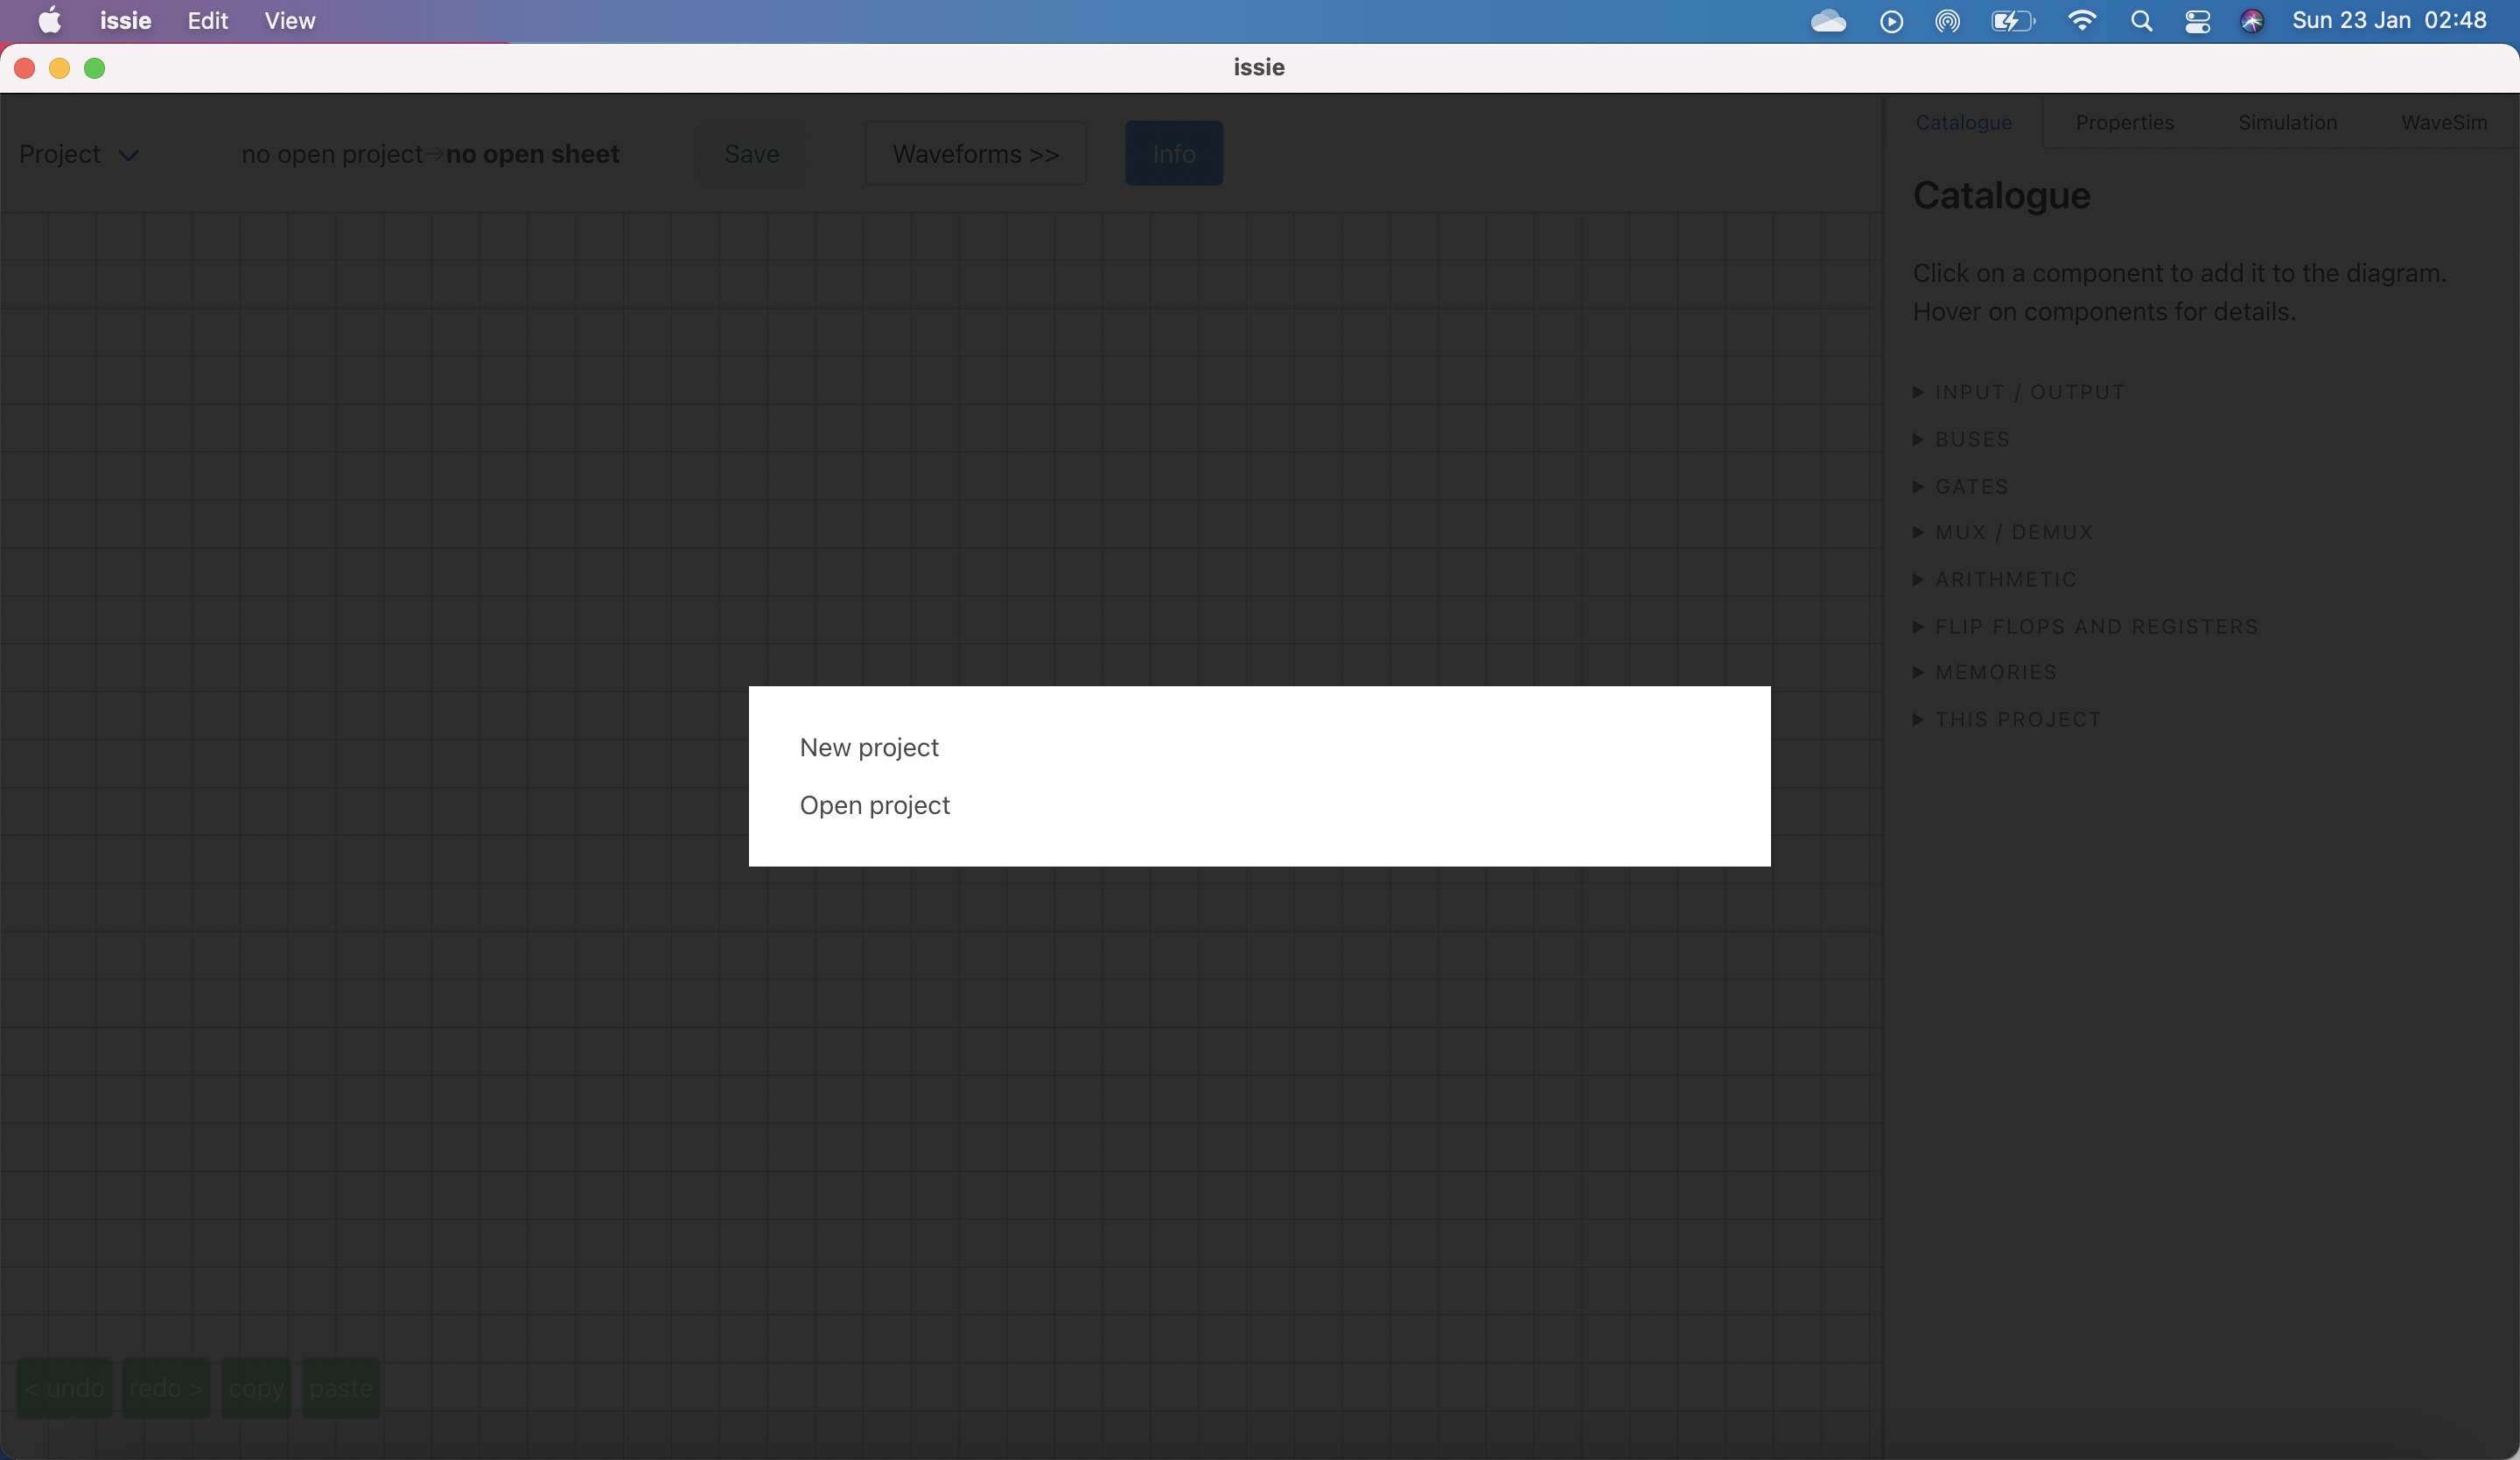
\includegraphics[width=\textwidth]{Appendices/IssieOpening.png}
    \caption{Issie's opening screen}
    \label{fig:IssieOpen}
\end{figure}

\begin{figure} [h]
    \centering
    \includegraphics[width=\textwidth]{Appendices/IssieSheetAnnotated.png}
    \caption{A sheet (schematic) open in Issie, with a component and wire selected}
    \label{fig:IssieSheetAnnotated}
\end{figure}

\begin{figure} [h]
    \centering
    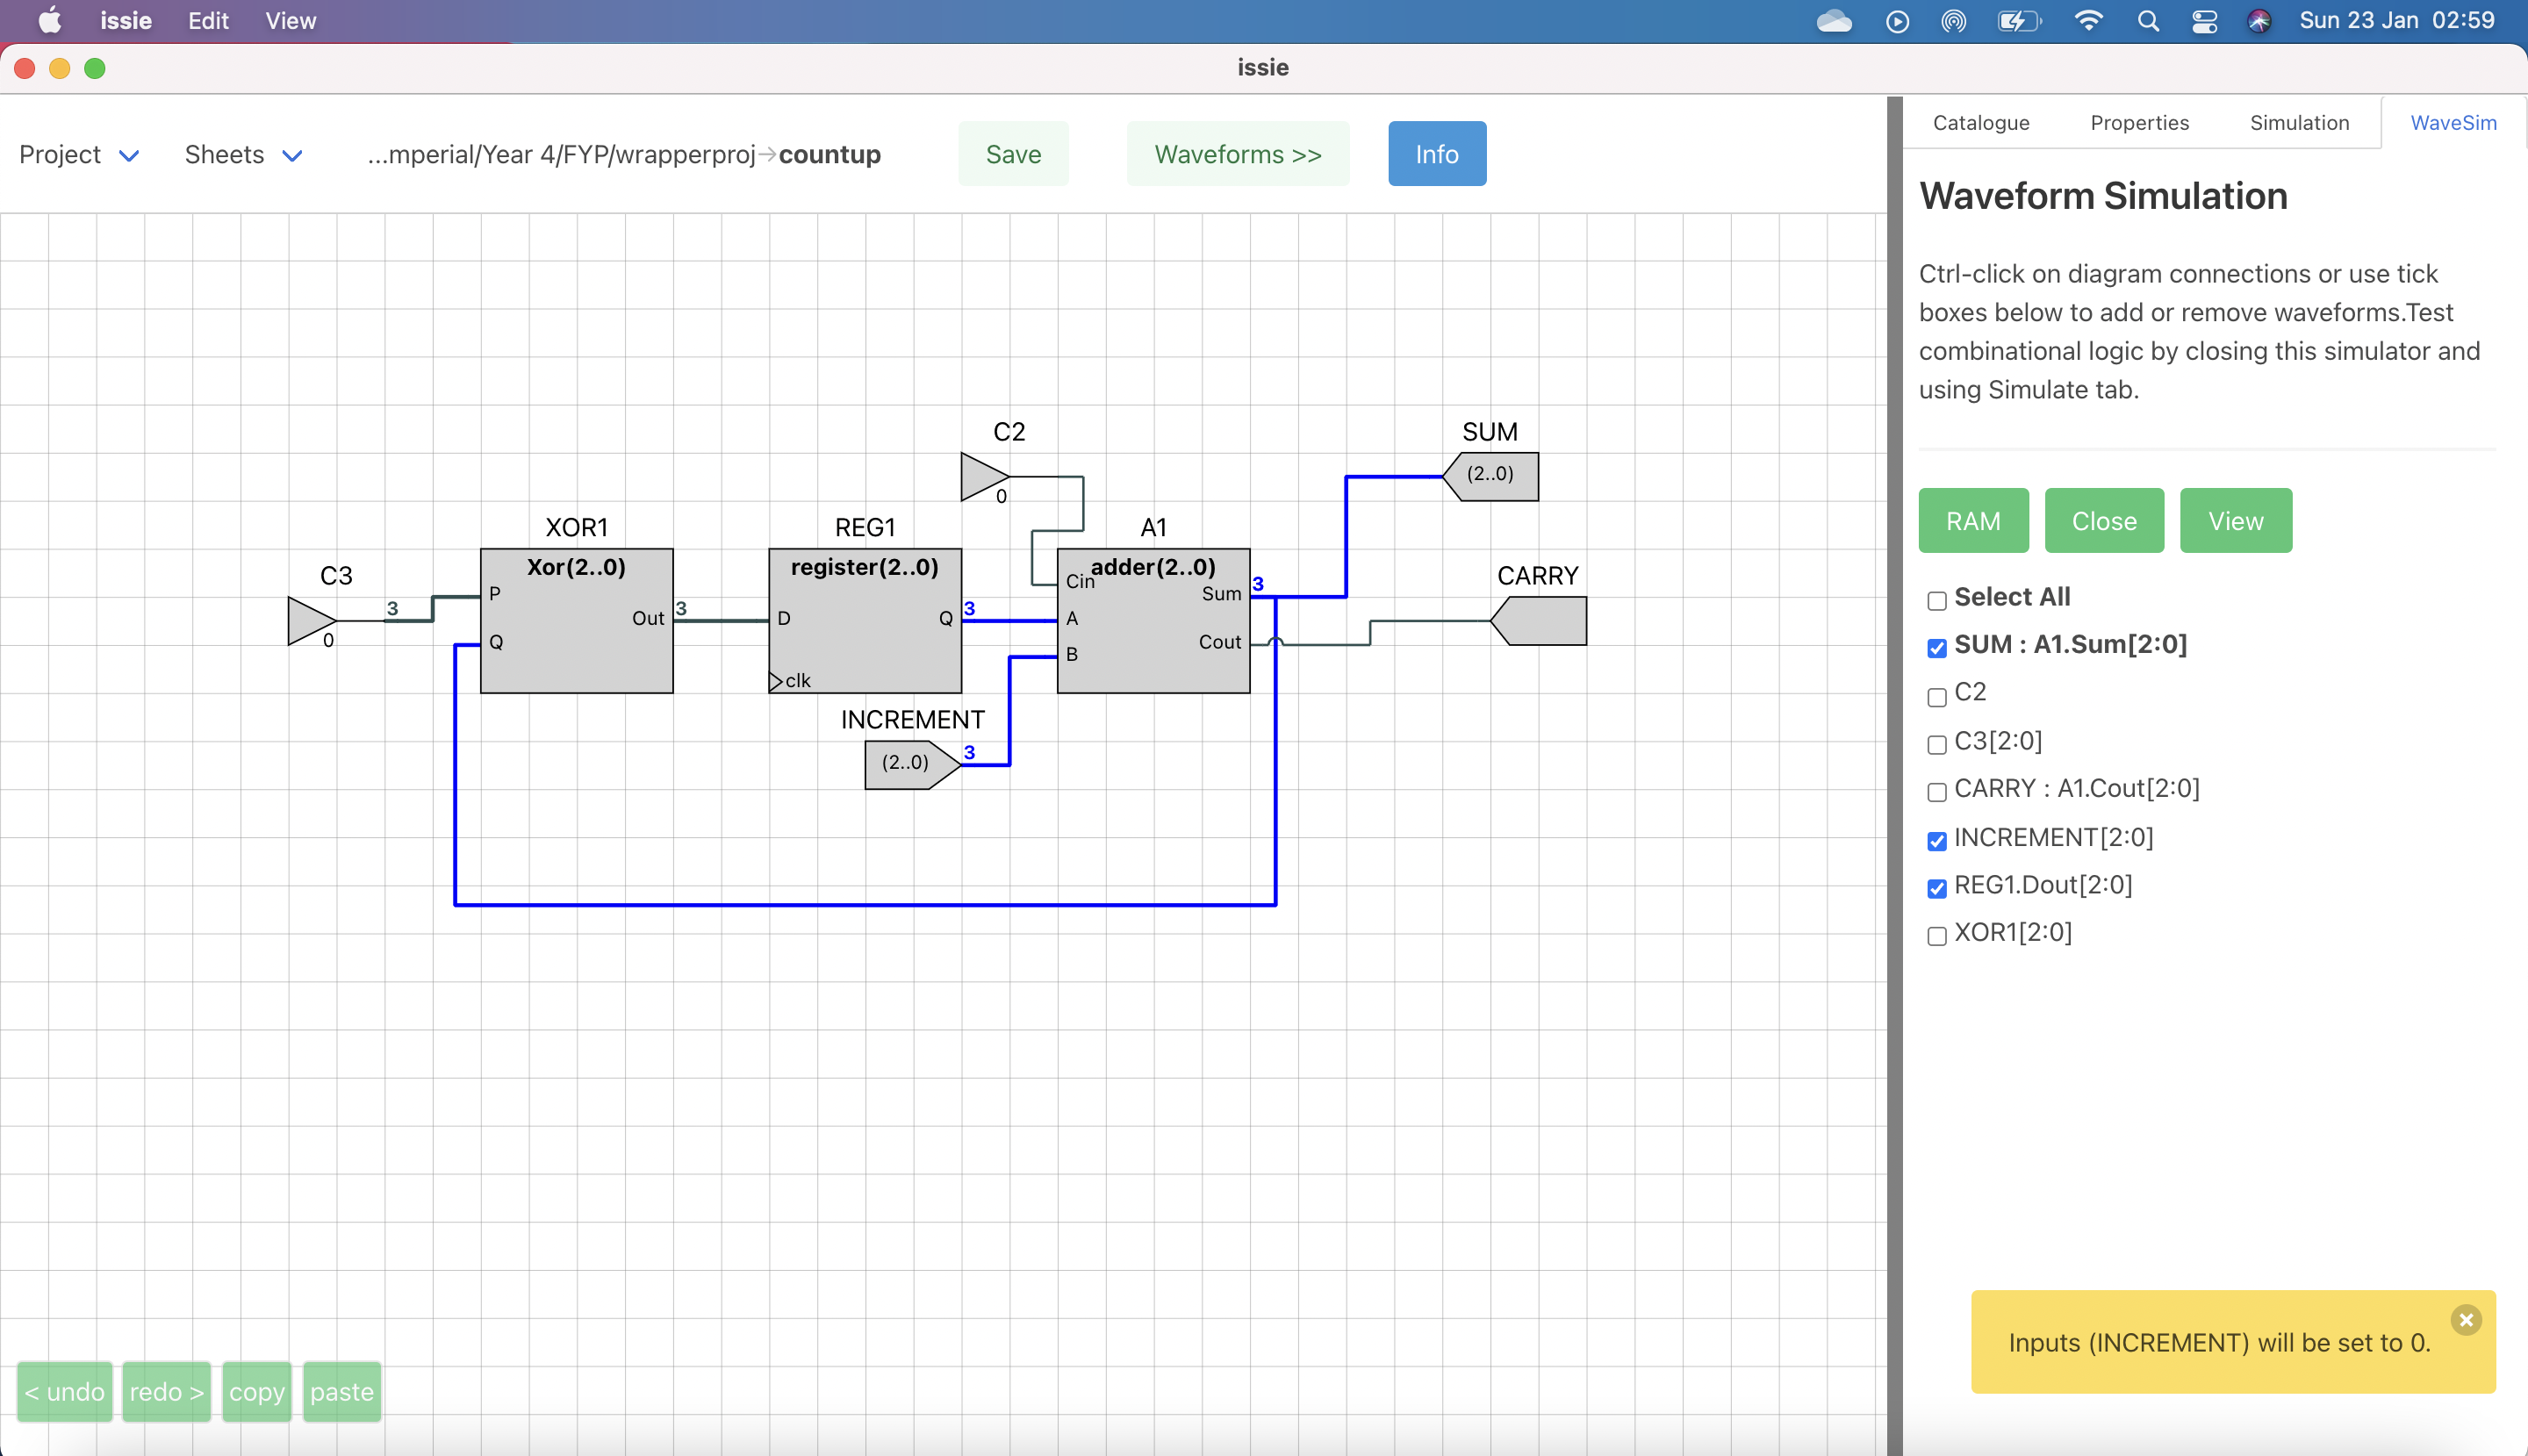
\includegraphics[width=\textwidth]{Appendices/IssieWaveSimSel.png}
    \caption{Issie's Waveform Simulator selection menu}
    \label{fig:IssieWSSel}
\end{figure}

\begin{figure} [h]
    \centering
    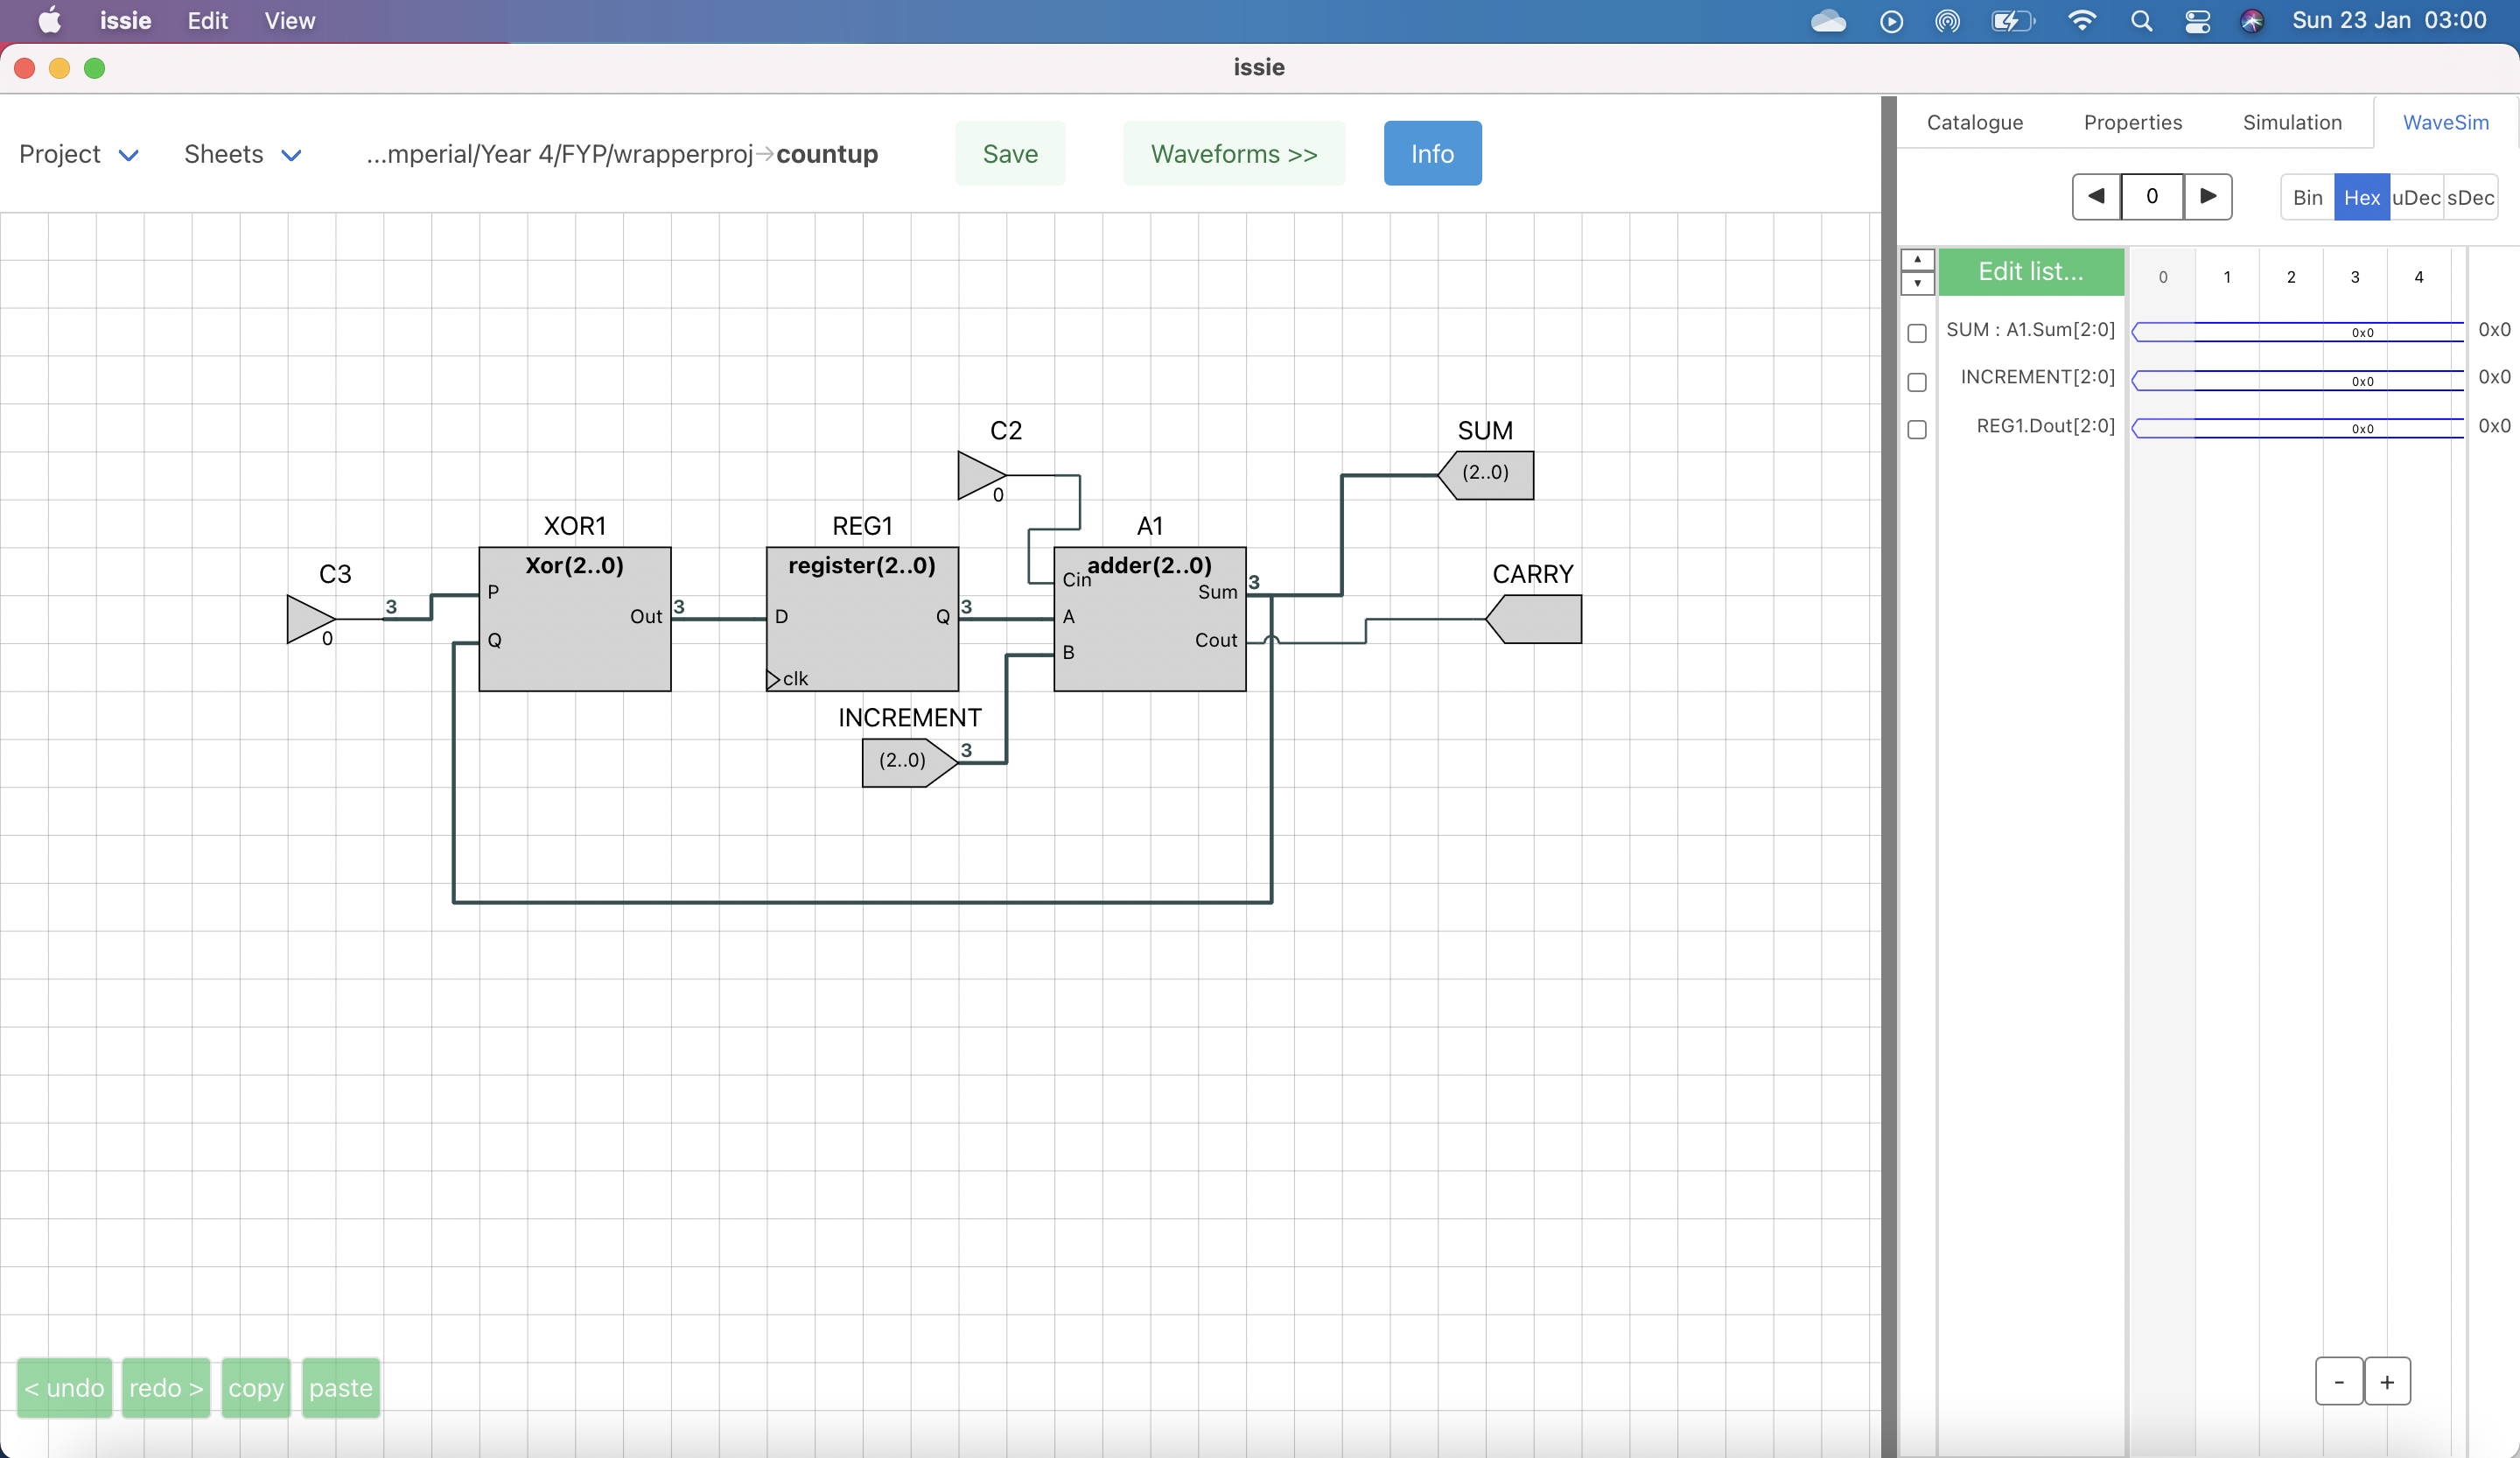
\includegraphics[width=\textwidth]{Appendices/IssieWaveSim.png}
    \caption{Issie's Waveform Simulator}
    \label{fig:IssieWS}
\end{figure}


\end{document}
